%%%%%%%%%%%%%%%%%%%%%%%%%%%%%%%%%
% Main File                     %
%%%%%%%%%%%%%%%%%%%%%%%%%%%%%%%%%
%
% This is the main file of your report. It serves as the starting point and controls the overall structure of your document. Unless you want to add or remove a section, there is usually no need to modify this file.

% Customize the content of the main file by including the necessary sections using the \input command. Each section has its own file, which contains the specific content for that section.

%%%%%%%%%%%%%%%%%%%%%%%%%%%%%%%%%

\documentclass[10pt]{article}

%%%%%%%%%%%%%%%%%%%%%%%%%%%%%%
% Preamble of the project    %
%%%%%%%%%%%%%%%%%%%%%%%%%%%%%%
%
% This file contains the preamble of the project, which includes various packages and settings to customize the document layout, formatting, and styling.

% Make sure to include necessary packages for mathematical symbols, graphics, page layout,
% captions, section headings, lists, hyperlinks, tables, bibliography, and other functionalities.
%
% Remember to update the bibliography file, and include any abbreviations or acronyms needed for your project.
%%%%%%%%%%%%%%%%%%%%%%%%%%%%%%


% Packages
\usepackage{amssymb} % For mathematical symbols
\usepackage{graphicx} % For including graphics in the document
\usepackage{geometry} % For customizing page layout and margins
\usepackage{titling} % For customizing the title
\usepackage{caption} % For customizing captions
\usepackage{subcaption} % For subcaptions
\usepackage{array} % For customizing table column formatting
\usepackage{hyperref} % For creating hyperlinks within the document
\usepackage{titlesec} % For customizing section headings
\usepackage{enumitem} % For customizing enumerated and itemized lists
\usepackage{float} % For customizing floating objects like figures and tables
\usepackage{tikz} % For creating graphics and diagrams
\usepackage{changepage} % For making changes to page layout within the document
\usepackage{indentfirst} % For indenting the first paragraph after section headings
\usepackage{xcolor} % For customizing text and background colors
\usepackage[nottoc]{tocbibind} % For including lists in the table of contents
\usepackage{acronym} % For creating a list of abbreviations
\usepackage{setspace} % For adjusting spacing
\usepackage{fontspec} % For customizing font
\usepackage{fancyhdr} % For customizing page headers and footers
\usepackage{ragged2e} % For text alignment
\usepackage[style=ieee]{biblatex} % For IEEE referencing style
\usepackage{tikz}
\usetikzlibrary{positioning, shapes, arrows, positioning,arrows.meta,calc,decorations.pathreplacing}
\usepackage[ruled,vlined,linesnumbered]{algorithm2e}
\SetKwInput{KwInput}{Input}
\SetKwInput{KwOutput}{Output}
\usepackage{tikz}
\usetikzlibrary{shapes.geometric, arrows.meta, positioning}
\usepackage{adjustbox}


% Spacing
\setstretch{1.5}

% Font
\setmainfont{CenturyGothic.ttf}[
    BoldFont=CenturyGothicbold.ttf,
    BoldItalicFont=CGOTHICBI.ttf,
    ItalicFont=gothici.ttf
]

% Titling
\titleformat*{\section}{\fontsize{16pt}{19.2pt}\bfseries\headingfont\MakeUppercase}
\titleformat*{\subsection}{\fontsize{13pt}{15.6pt}\bfseries\headingfont}
\titleformat*{\subsubsection}{\fontsize{13pt}{15.6pt}\bfseries\headingfont}

% Subsubsubsection Command
\newcommand{\subsubsubsection}[1]{%
  %\par\addvspace{3.25ex plus 1ex minus .2ex}%
  {\normalfont\fontsize{12pt}{14pt}\selectfont\bfseries\itshape #1}%
  \par\addvspace{1.5ex plus .2ex}%
}

% Subsubsubsubsection Command
\newcommand{\subsubsubsubsection}[1]{%
  \par\addvspace{3.25ex plus 1ex minus .2ex}%
  {\normalfont\fontsize{10pt}{12pt}\selectfont\bfseries\itshape #1}%
  \par\addvspace{1.5ex plus .2ex}%
}

% Adjust spacing options
\titlespacing*{\section}{0pt}{2\baselineskip}{0.5\baselineskip}
\titlespacing*{\subsection}{0pt}{1\baselineskip}{0.5\baselineskip}
\titlespacing*{\subsubsection}{0pt}{1\baselineskip}{0.5\baselineskip}
\titlespacing*{\subsubsubsection}{0pt}{1\baselineskip}{0.5\baselineskip}
\titlespacing*{\subsubsubsubsection}{0pt}{1\baselineskip}{0.5\baselineskip}

% Format \section
\titleformat{\section}
{\fontsize{16pt}{19pt}\selectfont\bfseries\MakeUppercase}
{\thesection}
{0.5em}
{}

% Format \subsection
\titleformat{\subsection}
{\fontsize{13pt}{15.6pt}\selectfont\bfseries}
{\thesubsection}
{0.5em}
{}

% Format \subsubsection
\titleformat{\subsubsection}
{\fontsize{13pt}{15.6pt}\selectfont\bfseries}
{\thesubsubsection}
{0.5em}
{}

% Format \subsubsubsection
\titleformat{\subsubsubsection}
{\fontsize{12pt}{14pt}\selectfont\bfseries\itshape}
{}
{0em}
{}

% Format \subsubsubsubsection
\titleformat{\subsubsubsubsection}
{\fontsize{10pt}{12pt}\selectfont\bfseries\itshape}
{}
{0em}
{}

% Margins
\geometry{margin=2.5cm}

% Justification
\justifying

% Pagination
\pagestyle{fancy}
\fancyhf{}
\rfoot{\thepage}
\renewcommand{\headrulewidth}{0pt}
\renewcommand{\footrulewidth}{0pt}

% Set paragraph indentation
\setlength{\parindent}{1.27cm}

% Customize caption format for figures and tables
\captionsetup{skip=0pt}

% Change the title of the table of contents
\renewcommand{\contentsname}{Table of Contents}

% Bibliography
\addbibresource{references.bib}

\usepackage{graphicx}
\usepackage{caption} % Required for customizing the captions

\DeclareCaptionLabelFormat{bold}{\textbf{#1 #2}} % Define a bold caption label format
\captionsetup[figure]{labelformat=bold} % Apply the bold format to figure captions
\usepackage{tocloft} % Required for customizing the table of contents and lists of figures/tables

% Redefine the format for figure entries in the List of Figures
\renewcommand{\cftfigpresnum}{\bfseries\figurename\enspace}
\renewcommand{\cftfigaftersnum}{\bfseries:}

% Set the width of the figure number to accommodate "Figure 10:" properly
\usepackage{tocloft}
\usepackage{calc} % for \widthof
\usepackage{amsmath}
\usepackage{multirow}
% make only the label bold, not the caption text
\renewcommand{\cftfigpresnum}{\textbf{Figure~}}
\renewcommand{\cftfigaftersnum}{\textbf{:}\space}

% set the number column wide enough (adjust 99 if you have more than 99 figures)
\setlength{\cftfignumwidth}{\widthof{\textbf{Figure~99: }}}





% Include the preamble file, which contains the necessary packages and settings for customizing the document layout and formatting.

\begin{document}

%%%%%%%%%%%%%%%%%%%%%%%%%%%%%%%%%
% Title Page                    %
%%%%%%%%%%%%%%%%%%%%%%%%%%%%%%%%%

\begin{titlepage}
    \centering
    
    %--- Logo ---
    % Ensure the path is correct. If the image is in a subfolder, use 'images/filename'
    \includegraphics[width=6cm]{images/medtech-logo.png} \\
    
    \vspace{0.5cm}
    
    %--- Department / Report Type ---
    {\Large \textbf{SOFTWARE ENGINEERING}} \\ 
    \vspace{0.2cm}
    {\Large \textbf{FINAL REPORT}} \\
    
    \vspace{1.5cm}
    
    %--- Project Title ---
    {\Large \textbf{Neural Inversion of Synthesizer Parameters from Audio: A Comparative Study of Convolutional and Transformer Architectures}} \\
    
    \vspace{1.5cm}
    
    %--- Author ---
    {\large \textbf{BY}} \\
    \vspace{0.2cm}
    {\large \textbf{Marouane Ben Haj Hassine}} \\
    
    \vspace{1.5cm}
    
    %--- Supervisors ---
    % Note: Since the supervisor is the same for both, you might consider combining them, 
    % but I have kept them separate as per your original layout.
    
    \textbf{ACADEMIC SUPERVISOR} \\
    \vspace{0.1cm}
    Dr. Ahmed Khanfir \\
    
    \vspace{0.8cm}
    
    \textbf{INSTITUTION SUPERVISOR} \\
    \vspace{0.1cm}
    Dr. Ahmed Khanfir \\
    
    \vspace{1.0cm}
    
    %--- Institution / Research Center ---
    \textbf{Mediterranean Institute of Technology Research Center} \\
    \vspace{0.3cm}
    \includegraphics[width=4cm]{images/medtech-logo.png} 
    % If the research center has a different logo, update the filename above.
    
    \vfill
    
    %--- Date ---
    {\normalsize \textbf{Tunis, 2024 - 2025}}

\end{titlepage}
% Include the title page file, which contains the code for the title page of your project.

\pagenumbering{roman}
% Set the page numbering to lowercase Roman numerals for the preliminary sections.

\phantomsection
\input{Preliminary Files/approval}
\clearpage
% Include the approval section.

\phantomsection
\input{Preliminary Files/declaration}
\clearpage
% Include the declaration section.

\phantomsection
\input{Preliminary Files/work-term}
\clearpage
% Include the work term section.

\phantomsection
\section*{Abstract}

\noindent
The inverse synthesis problem, recovering synthesizer parameters from audio, is inherently ill-posed, as multiple parameter configurations can produce perceptually similar outputs. This ambiguity, combined with nonlinear parameter interactions, makes manual sound reproduction a time-consuming task for music producers. We investigate the feasibility of learning this inverse mapping using deep learning.

\noindent \newline
To address this challenge, we propose a supervised regression framework using a custom dataset generated programmatically via the Pedalboard library, driving Vital, an open-source and widely used wavetable synthesizer. We restrict the parameter space to 16 synthesis parameters covering oscillators, envelopes, filters, and effects, keeping the task tractable while retaining musical relevance.

\noindent \newline
Our experiments progress across three iterations. In V1, we compare three architectures: a custom residual Convolutional Neural Network (CNN), ConvNeXt, and an Audio Spectrogram Transformer (AST), on a single-scale mel spectrogram input, establishing ConvNeXt and AST as the strongest candidates. In V2, we advance both architectures with three-scale mel spectrogram input (fine, mid, coarse), Feature-wise Linear Modulation (FiLM) pitch conditioning, and a grouped prediction head, trained on the same dataset. In V3, we further improve upon V2 via multi-pitch rendering per preset and Spectrogram Augmentation (SpecAugment) regularisation on a significantly expanded dataset.

\noindent \newline
We find that multi-scale spectrograms provide richer timbral information, yielding significant Mean Absolute Error (MAE) improvements for both ConvNeXt and AST from V1 to V2, though we observed signs of overfitting at this stage. In V3, we show that multi-pitch rendering and SpecAugment effectively mitigate overfitting and, crucially, activate FiLM pitch conditioning, which had proven ineffective in V2 due to single-pitch data. On a shared 100-sample evaluation set, we observe that ConvNeXt-tiny achieves MAE 0.0739 in V2 versus 0.0755 for AST; in V3, AST narrows this gap to achieve MAE 0.0525 vs.\ 0.0530 for ConvNeXt, with AST also leading on the Multi-Scale Spectral loss (1.10 vs.\ 1.22), suggesting that global self-attention becomes increasingly advantageous with greater data diversity.

\noindent \newline
\textbf{Keywords:} Audio Inversion --- Sound Synthesis --- Deep Learning --- Parameter Estimation --- Mel-Spectrogram --- Neural Audio Processing

\clearpage
% Include the abstract section.

\phantomsection
\section*{Acknowledgements}
I want to express my sincere gratitude to the people and institutions whose advice and assistance were crucial to the accomplishment of this capstone project.

\noindent \newline
I want to thank my supervisor, \textbf{Dr. Ahmed Khanfir}, from the bottom of my heart. His guidance and directions during the process were really helpful in conceiving this research. I have always been inspired by Dr. Ahmed Khanfir, who has shared knowledge and insightful remarks that go beyond the project's technical goals. Along with recommending this internship, his words of support and encouragement have been major sources of motivation for me.

\noindent \newline
I would also like to extend my sincere gratitude to \textbf{SMU's Research Center} for their hospitality and for providing the resources and infrastructure necessary to carry out this work. I am equally thankful to all its members for their helpfulness, availability, and the welcoming environment they created throughout this experience.

\noindent \newline
Finally, I want to wholeheartedly thank my family and friends, whose unwavering support and encouragement have carried me to this point in my journey. A special thank you goes to my cousin \textbf{Khalil Riahi}, who generously provided access to his GPU, enabling me to experiment and iterate on my models from home — your help made a real difference.

\addcontentsline{toc}{section}{Acknowledgements}

\vspace{1.4cm}
\noindent
\clearpage
% Include the acknowledgements section.

\normalsize

\tableofcontents
\clearpage
% Include the table of contents, which lists the sections and subsections of your project.

\phantomsection
\listoftables
\clearpage
% Include the list of tables, which lists all the tables in your project.

\phantomsection
\listoffigures
\clearpage
% Include the list of figures, which lists all the figures in your project.

\phantomsection
\makeatletter
\section*{\listequationsname}
\addcontentsline{toc}{section}{\listequationsname}
\@starttoc{loe}
\makeatother
\clearpage
% Include the list of equations, which lists all named equations in your project.

\phantomsection
\section*{List of Abbreviations}

\begin{itemize}
    \item \textbf{AMP} : Automatic Mixed Precision
    \item \textbf{AdamW} : Adaptive Moment Estimation with Weight Decay
    \item \textbf{AST} : Audio Spectrogram Transformer
    \item \textbf{CNN} : Convolutional Neural Network
    \item \textbf{ConvNeXt} : Convolutional Neural Network in the Style of Vision Transformers
    \item \textbf{CLS} : Classification Token (Transformer)
    \item \textbf{dB} : Decibels
    \item \textbf{DDSP} : Differentiable Digital Signal Processing
    \item \textbf{DFT} : Discrete Fourier Transform
    \item \textbf{DSP} : Digital Signal Processing
    \item \textbf{FFN} : Feed-Forward Network
    \item \textbf{FFT} : Fast Fourier Transform
    \item \textbf{FiLM} : Feature-wise Linear Modulation
    \item \textbf{FM} : Frequency Modulation
    \item \textbf{GA} : Genetic Algorithm
    \item \textbf{GELU} : Gaussian Error Linear Unit
    \item \textbf{JSON} : JavaScript Object Notation
    \item \textbf{JSONL} : JSON Lines
    \item \textbf{LFO} : Low-Frequency Oscillator
    \item \textbf{LR} : Learning Rate
    \item \textbf{MAE} : Mean Absolute Error
    \item \textbf{mel} : Mel Scale (perceptual frequency scale)
    \item \textbf{MHSA} : Multi-Head Self-Attention
    \item \textbf{MIDI} : Musical Instrument Digital Interface
    \item \textbf{MIR} : Music Information Retrieval
    \item \textbf{MLP} : Multi-Layer Perceptron
    \item \textbf{MSS} : Multi-Scale Spectral Loss
    \item \textbf{NFT} : Normalising Flow Transform
    \item \textbf{ReLU} : Rectified Linear Unit
    \item \textbf{RMS} : Root Mean Square
    \item \textbf{SpecAugment} : Spectrogram Augmentation
    \item \textbf{STFT} : Short-Time Fourier Transform
    \item \textbf{VCA} : Voltage-Controlled Amplifier
    \item \textbf{VCF} : Voltage-Controlled Filter
    \item \textbf{VCO} : Voltage-Controlled Oscillator
    \item \textbf{ViT} : Vision Transformer
    \item \textbf{VST} : Virtual Studio Technology
    \item \textbf{WAV} : Waveform Audio File Format
\end{itemize}

\clearpage

\pagenumbering{arabic}
% Set the page numbering to Arabic numerals for the main sections.


%%%%%%%%%%%%%%%%%%%%%%%%%%%%%%%%%
% Introduction                  %
%%%%%%%%%%%%%%%%%%%%%%%%%%%%%%%%%

\section{INTRODUCTION}
\label{sec:introduction}

This section provides an overview of the conducted research, starting with the project context, followed by the purpose of the study, research objectives, research questions, and the approach and boundaries that define the scope of this work.

\subsection{Project Context}

Sound synthesis is a fundamental component of modern music production and cinematic sound design, enabling the creation of complex, rich sonic textures as well as faithful emulations of acoustic instruments and sounds found in nature. While synthesis can be achieved through purely acoustic means, synthesizers have become one of the primary tools for this purpose. At their core, synthesizers expose a structured interface of parameters, including oscillators, filters, envelopes, modulation routings, and effects, whose combined interaction shapes the output sound. The relationship between these parameters and the resulting audio is highly nonlinear and unintuitive, making manual sound reproduction a time-consuming process \cite{roads1996computer, cook2002realsound}.

\par \vspace{0.5cm}

\noindent Historically, the most culturally influential synthesizers, namely the Minimoog by Moog and the Prophet-5 by Sequential Circuits, featured a fixed signal flow with a comparatively small number of parameters. Despite this simplicity, these instruments remain widely used in modern music production and are capable of expressing a surprisingly wide range of sounds. This stands in contrast to modern software synthesizers such as Vital by Matt Tytel \cite{tytel2020vital}, Serum by Xfer Records, or Diva by u-he, which expose hundreds of parameters, many of which remain unexplored in practice. Notably, even when working with these feature-rich instruments, producers tend to gravitate toward a familiar and interpretable subset: oscillator waveforms, envelope shapes, filter cutoff, and a few modulation amounts. This observation led us to restrict the parameter space in this study to a curated subset inspired by those vintage signal chains, keeping the task both musically meaningful and tractable.

\par \vspace{0.5cm}

\noindent In this project, we focus on Vital, a modern open-source wavetable synthesizer developed by Matt Tytel and widely adopted in the music production community, making it an ideal subject for this research. Our motivation is straightforward: a producer who hears a sound they want to recreate, whether from a reference track or their own imagination, typically faces a time-consuming process of manual programming. An automated estimation system would serve as a shortcut for beginners and a time-saving tool for experienced sound designers alike. More broadly, it can act as a creative aid: feeding an arbitrary audio signal into the estimator yields a synthesizer approximation that can open timbral directions difficult to discover through manual exploration.

\par \vspace{0.5cm}

\noindent The task of recovering synthesizer parameters from audio, known as inverse synthesis, has been studied since the early days of computational audio. Initial approaches relied on Genetic Algorithms (GA) \cite{walker2007audiosynthesis}, which are computationally expensive and scale poorly to high-dimensional parameter spaces. Deep learning later shifted the paradigm toward direct regression \cite{yeeking2018automatic, barkan2019inversynth}, removing the need for iterative synthesis at inference time. More recently, architectures from computer vision have been adapted for audio: Convolutional Neural Networks (CNNs) on mel-spectrograms have become a standard baseline \cite{hershey2017cnn}, and the Audio Spectrogram Transformer (AST) has shown strong results using global self-attention \cite{gong2021ast}. The work most directly related to this project is that of Bruford et al. \cite{bruford2024ast}, who applied AST to synthesizer sound matching and established a strong transformer baseline for the task.

\subsection{Purpose of the Study}

The purpose of this work is to evaluate how effectively existing deep learning architectures can estimate synthesizer parameters directly from audio, comparing them under a shared dataset and experimental setup. To support this, we design and implement a modular training and evaluation framework applicable to multiple architectures and training configurations, using the Vital synthesizer throughout. Audio samples are generated programmatically by driving Vital through the Pedalboard library under controlled rendering conditions; each sample is paired with its ground-truth parameter vector and the Musical Instrument Digital Interface (MIDI) pitch at which it was rendered. The dataset is built in two stages: an initial generated version and a subsequently augmented version three times larger, obtained by rendering each preset at multiple MIDI pitches. Across three experimental iterations of increasing complexity, we compare three neural architectures: a residual CNN baseline \cite{he2016resnet} (first iteration only), a ConvNeXt backbone \cite{liu2022convnext}, and an AST \cite{gong2021ast}, tracing the contributions of multi-scale mel input, Feature-wise Linear Modulation (FiLM)-based pitch conditioning \cite{perez2018film}, and multi-pitch data augmentation to overall estimation accuracy.

\subsection{Research Objectives}

The following objectives define the scope of this work:

\begin{itemize}

\item[$\blacksquare$] \textbf{Objective 1:} Evaluate and compare three deep learning architectures, namely a residual CNN baseline, ConvNeXt, and AST, in their ability to regress synthesizer parameters from mel-spectrogram inputs, and identify which architectural family is best suited to this task.

\item[$\blacksquare$] \textbf{Objective 2:} Assess whether a multi-scale mel-spectrogram input combining fine, mid, and coarse time-frequency resolutions provides a measurable improvement over a single-scale mel-spectrogram for synthesizer parameter estimation.

\item[$\blacksquare$] \textbf{Objective 3:} Investigate the conditions under which FiLM-based pitch conditioning improves parameter estimation accuracy, and determine how the availability of multi-pitch training data affects its effectiveness.

\end{itemize}

\subsection{Research Questions}

\begin{itemize}

    \item[$\blacksquare$] \textbf{Research Question 1:} How do convolutional architectures (residual CNN and ConvNeXt) compare to AST in regressing synthesizer parameters from mel-spectrograms? \\
    \textbf{Rationale:} CNNs build up representations by stacking local convolutions, while transformers reason globally through self-attention across the entire input. These are fundamentally different inductive biases, and it is not obvious which one better serves a synthesizer parameter regression task. Synthesized sounds tend to be characterized by localized spectral structures such as harmonic stacks, filter shapes, and envelope transients, which intuitively favor local feature extraction. Whether this holds in practice, and by how much, is what this comparison aims to settle.

    \item[$\blacksquare$] \textbf{Research Question 2:} Does replacing a single mel-spectrogram with a three-scale representation combining fine, mid, and coarse spectrograms improve synthesizer parameter estimation accuracy? \\
    \textbf{Rationale:} Any single mel-spectrogram is a resolution compromise: you cannot simultaneously maximize temporal and spectral precision. This matters because synthesizer parameters operate at different timescales: a fast attack is best seen in a fine-resolution spectrogram, while harmonic texture and filter shape are more legible at coarser frequency resolution. Providing all three scales as a stacked input is a practical way to sidestep this trade-off, and this question tests whether doing so actually translates to better parameter estimates.

    \item[$\blacksquare$] \textbf{Research Question 3:} Under what conditions does FiLM-based pitch conditioning improve synthesizer parameter estimation, and why does its effectiveness depend on the training data? \\
    \textbf{Rationale:} The frequency content of a synthesized note depends on both its synthesis parameters and the MIDI pitch at which it is played. A model trained on single-pitch renders never sees the same preset at different pitches, so there is no signal pushing it to make use of the pitch input. The hypothesis is that multi-pitch rendering, where each preset is rendered at several MIDI notes, forces the model to learn pitch-invariant parameter representations and gives the FiLM conditioning a meaningful role. This question tests that hypothesis directly.

\end{itemize}

\subsection{Approach and Boundaries of the Study}

This research is structured around the Design Science Research (DSR) methodology \cite{wieringa2014design}. DSR is a problem-solving paradigm centered on the creation and evaluation of purposeful artifacts; here, those artifacts are the deep learning models and the data generation pipeline built to support them. Its iterative cycle of problem investigation, design, implementation, and evaluation fits naturally with how this project developed: each experimental iteration (V1, V2, V3) refined the system based on what the previous one revealed.

\subsubsection{Scope}
Three neural architectures are compared: a residual CNN serving as a V1 reference, ConvNeXt, and AST, all applied to synthesizer parameter regression on the Vital synthesizer. The comparison covers single-scale and multi-scale mel-spectrogram inputs, FiLM-based pitch conditioning, grouped prediction heads, and multi-pitch data augmentation across three experimental iterations. We report Mean Absolute Error (MAE) in the normalized parameter space, with 5-fold cross-validation and a per-parameter breakdown for each configuration. For V2 and V3, a Multi-Scale Spectral (MSS) loss computed on re-rendered audio serves as an additional perceptual evaluation metric.

\subsubsection{Limitations}
This investigation ran into several practical walls. GPU access was limited to a single NVIDIA RTX 4090 shared across multiple researchers; scheduling conflicts meant we could not run as many training experiments as we would have liked. The data pipeline added another layer of constraint: real-time audio rendering through Vital generated roughly 140 GB of raw Waveform Audio File Format (WAV) data, and the sheer time cost of rendering and validating every clip put a hard ceiling on how large the dataset could grow. The inverse synthesis literature also proved to be a narrow field, with few papers close enough to this work to serve as direct benchmarks. On top of that, the project sits at an unusual intersection of audio signal processing, music theory, and deep learning, and getting up to speed across all three required real effort from a team that came in primarily as software engineers.

\subsubsection{Delimitations}
The study is scoped to the Vital software synthesizer and the 16 parameters defined earlier. Generative architectures, recurrent networks, and reinforcement learning are out of scope; the focus is squarely on direct regression. Each preset is rendered as a 4-second audio clip. This duration was chosen because the target sounds are one-shots and sustained patches of the kind used in modern music production, where individual notes rarely extend beyond a few seconds. A 4-second window is sufficient to capture the full amplitude envelope of most patches, including pads with slow attacks and long decays. As a consequence of this fixed-duration render with no note-off event, the amplitude envelope sustain and release stages are never triggered and cannot be inferred from the audio; they are therefore excluded from the parameter set. Clips are stored in WAV rather than a lossy-compressed format such as Moving Picture Experts Group Audio Layer III (MP3), as compression introduces spectral artifacts that could corrupt the fine timbral detail the models are trained to predict. Although MSS loss has been used as a training objective in differentiable synthesis frameworks \cite{engel2020ddsp, caspe2022ddx7}, it is not used for training here. Vital is a non-differentiable black-box Virtual Studio Technology (VST) plugin, so computing MSS at each training step would require a differentiable proxy synthesizer, which is well beyond the scope of this work. MSS is therefore reserved as a post-hoc perceptual evaluation metric for V2 and V3. The study does not extend to analog hardware synthesizers, other VST plugins, or broader parameter spaces.

\subsubsection{Assumptions}
Three working assumptions underlie this study. First, the timbre-constrained generation strategy produces a dataset with sufficient coverage of musically meaningful sounds for the models to learn generalizable synthesis mappings. Second, the mel-spectrogram captures enough spectral and temporal information to characterize all 16 target parameters, even though phase information is discarded. Third, a reduction in normalized MAE is taken to correlate with a perceptually meaningful improvement in how closely the re-rendered output matches the target sound.

\subsection{Contributions}

This work makes the following contributions to the field of inverse synthesis and audio deep learning:

\begin{itemize}

\item[$\blacksquare$] \textbf{First direct comparison of ConvNeXt and AST for synthesizer parameter estimation.} Prior work has applied AST to sound matching \cite{bruford2024ast} or convolutional models to parameter regression \cite{barkan2019inversynth}, but no study has directly compared these two architectural families in the same controlled experimental setting.

\item[$\blacksquare$] \textbf{First use of explicit pitch conditioning for synthesizer parameter regression.} A MIDI pitch input is incorporated as an auxiliary conditioning signal via FiLM modulation, enabling the model to disentangle fundamental frequency from timbral characteristics. This conditioning strategy has not previously been explored for this task.

\item[$\blacksquare$] \textbf{Multi-scale mel spectrogram as a three-channel input representation.} To the best of our knowledge, stacking fine, mid, and coarse mel spectrograms into a single multi-channel input tensor has not previously been applied to synthesizer parameter estimation, and its benefit over single-scale input is evaluated through a dedicated ablation.

\item[$\blacksquare$] \textbf{Timbre-constrained dataset generation methodology.} A structured dataset generation pipeline is proposed that constrains parameter sampling to musically coherent timbral families, ensuring coverage of practically relevant sounds while avoiding silent or pathological outputs.

\item[$\blacksquare$] \textbf{Open-source dataset generation pipeline for VST synthesizers.} The full Pedalboard-based rendering pipeline, including timbre-constrained preset generation, silence filtering, and multi-scale mel extraction, is released as open-source code. The pipeline is designed to be extensible: new parameters can be added to the generation schema with minimal configuration, making it straightforward to expand the parameter space or adapt the pipeline to other VST synthesizers. To our knowledge, no prior inverse synthesis work has publicly released a comparable VST-driven dataset generation framework.

\item[$\blacksquare$] \textbf{Open-source training and evaluation framework.} The complete experimental codebase, including all model architectures, training configurations, ablation variants, and cross-validation splits, is made publicly available, enabling direct reproduction and extension of all results reported in this study.

\end{itemize}

\subsection{Structure}

The remainder of this report is organized as follows. Section 2 establishes the theoretical background and reviews prior work in sound synthesis, inverse synthesis methods, and the deep learning architectures used in this study. Section 3 describes the research methodology, detailing the DSR framework applied, the data generation pipeline, and the experimental setup. Section 4 presents the three experimental iterations — V1, V2, and V3 — describing the design decisions, architectural choices, and incremental improvements introduced at each stage. Section 5 reports the quantitative results and findings across all experiments. Section 6 discusses the results in light of the research questions, addresses limitations, and interprets per-parameter performance patterns. Section 7 concludes the report by summarizing contributions and outlining directions for future work.

\clearpage
% Include the introduction section.

%%%%%%%%%%%%%%%%%%%%%%%%%%%%%%%%%
% Background and Literature Review
%%%%%%%%%%%%%%%%%%%%%%%%%%%%%%%%%

\section{BACKGROUND AND LITERATURE REVIEW}

This section establishes the theoretical and empirical foundations of this work. The background subsection introduces the key concepts in sound synthesis, the formal definition of the inverse synthesis problem, and the audio representations used as model inputs. The literature review then surveys prior work, moving from early optimization-based methods to modern deep learning approaches, and identifies the gap this study addresses.

\subsection{Background}

\subsubsection{Sound Synthesis and the Vital Synthesizer}

\subsubsubsection{A Brief History of Sound Synthesis}

The development of electronic sound synthesis spans six decades and four distinct technological paradigms, each shifting both the physics of sound generation and the sonic vocabulary of popular music \cite{roads1996computer}.

\par \vspace{0.3cm}

\noindent \textbf{Analog synthesis (1960s--1980s).} Robert Moog's demonstration of the first voltage-controlled synthesizer at the 1964 Audio Engineering Society convention established the foundational architecture that underlies all modern synthesizers: a voltage-controlled oscillator (VCO) generating a periodic waveform, a voltage-controlled filter (VCF) shaping its spectral content, and a voltage-controlled amplifier (VCA) imposing its dynamic envelope. The Minimoog Model D (1970) condensed this modular system into a portable, self-contained instrument whose normalled signal chain --- oscillators into filter into amplifier into effects --- remains the canonical template to this day. The ARP 2600 (1971) offered a semi-modular alternative prized for its patchable flexibility. The Prophet-5 (Sequential Circuits, 1978) introduced full programmability and patch memory to a polyphonic synthesizer, allowing sounds to be saved and recalled exactly --- a capability so fundamental that it is taken for granted in every instrument that followed \cite{cook2002realsound}.

\par \vspace{0.3cm}

\noindent These instruments defined the sonic palette of rock, funk, and early electronic music. Keith Emerson's Moog solo on ``Lucky Man'' by Emerson, Lake \& Palmer (1970) was one of the first widely heard synthesizer performances on a rock record. Stevie Wonder's \textit{Talking Book} (1972) and \textit{Innervisions} (1973) used the Minimoog as a primary melodic voice. Kraftwerk's ``Autobahn'' (1974) and Giorgio Moroder's sequenced Moog bassline on Donna Summer's ``I Feel Love'' (1977) established the synthesizer as a self-sufficient compositional medium. The ARP 2600 reached a different kind of cultural permanence: sound designer Ben Burtt used it to construct the voice of R2-D2 in \textit{Star Wars} (1977). The Prophet-5 contributed the thick polyphonic pads and brass stabs of synth-pop, heard across the work of Tears for Fears, Peter Gabriel, and New Order throughout the 1980s.

\par \vspace{0.3cm}

\noindent \textbf{Rhythm synthesis: the TR-808 and TB-303 (1980--1981).} Though not melodic synthesizers in the traditional sense, the Roland TR-808 drum machine and TB-303 bass line synthesizer represent milestone achievements in analog circuit-based sound generation. The TR-808 synthesized kick drums, snares, and hi-hats entirely from analog circuits rather than recorded samples, producing a distinctive deep kick and crisp rimshot that became the rhythmic foundation of hip-hop and electronic music. Afrika Bambaataa's ``Planet Rock'' (1982), Marvin Gaye's ``Sexual Healing'' (1982), and Prince's ``When Doves Cry'' (1984) brought the 808 to mainstream attention; it subsequently became the defining rhythmic voice of trap music. The TB-303 bass synthesizer, equipped with a resonant filter that could be driven to extreme squelching self-oscillation, gave an entire genre its name: Phuture's ``Acid Tracks'' (1987) launched acid house and, by extension, the lineage of techno and electronic dance music.

\par \vspace{0.3cm}

\noindent \textbf{FM and digital synthesis (1980s).} The Yamaha DX7 (1983) replaced analog circuits with six-operator frequency modulation (FM) synthesis, in which a set of digital oscillators modulate each other's frequencies to produce complex sideband-rich spectra unavailable to analog filters. The DX7 sold over 200,000 units, making it the best-selling synthesizer in history \cite{roads1996computer}, and its factory presets --- particularly the electric piano, slap bass, and marimba patches --- appeared on virtually every commercially released pop record between 1983 and 1990. A-ha's ``Take On Me'' (1985) and the prolific output of Quincy Jones's productions in this era are among the most recognizable examples. The Roland D-50 (1987) introduced linear arithmetic synthesis, blending short PCM attack transients with digital sustain bodies to produce lush, layered sounds that defined late-1980s new age and film scoring.

\par \vspace{0.3cm}

\noindent \textbf{Sample-based synthesis (late 1980s--2000s).} The Fairlight CMI (1979) and New England Digital Synclavier were the first instruments to store and play back arbitrary recorded waveforms at different pitches --- a paradigm shift from generating sound to reproducing it. Both were prohibitively expensive; Kate Bush used the Fairlight on ``Running Up That Hill'' (1985), and the Synclavier is audible across Michael Jackson's \textit{Thriller} (1982) productions. The Akai S950 and S1000 brought professional-quality sampling to a broader market and became central to 1990s hip-hop production. The Korg M1 (1988) combined sample playback with onboard effects and became the best-selling keyboard workstation of all time; its organ and piano presets are inseparable from the sound of early house music, heard on Black Box's ``Ride on Time'' (1989). This era shifted the craft of sound design from building timbres from physical first principles to selecting, layering, and processing recorded material.

\par \vspace{0.3cm}

\noindent \textbf{Software synthesis (1996--present).} Steinberg's VST (Virtual Studio Technology) standard in 1996 opened the digital audio workstation to third-party software instruments, eliminating the need for dedicated hardware. Software synthesizers could now implement any synthesis paradigm at negligible cost and with perfect parameter recall. Native Instruments, Arturia, and others recreated classic hardware digitally, free from tuning drift and with unlimited voices. Vital (Matt Tytel, 2020) represents the current endpoint of this trajectory: a free, open-source wavetable synthesizer that combines the classic analog signal chain with arbitrary wavetable oscillators, a deep modulation matrix, and programmatic parameter access via API. This evolution --- from a room-sized modular Moog to a synthesizer anyone can run on a laptop and control from a Python script --- is precisely what makes the inverse synthesis problem both tractable to study and practically relevant for working musicians.

\par \vspace{0.3cm}

\noindent Table~\ref{tab:synthesis_paradigms} summarises the four main synthesis paradigms discussed above.

\begin{table}[H]
\centering
\renewcommand{\arraystretch}{1.4}
\begin{tabular}{p{2.6cm} p{2.8cm} p{4.2cm} p{4.0cm}}
\hline
\textbf{Era} & \textbf{Paradigm} & \textbf{Key Instruments} & \textbf{Core Mechanism} \\
\hline
1960s--1980s & Analog subtractive & Moog Modular, Minimoog, ARP 2600, Prophet-5 & VCO waveforms shaped by VCF and VCA via continuous voltage control \\
1980s & FM / digital & Yamaha DX7, Roland D-50 & Digital oscillators modulating each other's frequencies to produce sideband-rich spectra \\
Late 1980s--2000s & Sample-based & Fairlight CMI, Akai S-Series, Korg M1 & PCM recordings played back at different pitches and shaped by digital filters \\
1996--present & Software (VST) & Native Instruments, Arturia, Vital & Any synthesis algorithm running inside a DAW with no dedicated hardware \\
\hline
\end{tabular}
\vspace{0.3cm}
\caption{The four main sound synthesis paradigms from the analog era to modern software synthesizers.}
\label{tab:synthesis_paradigms}
\end{table}

\subsubsubsection{Physics of Electronic Sound Generation}

Understanding the physical mechanisms behind synthesis is essential for interpreting which properties of an audio representation carry the most information for parameter estimation.

\par \vspace{0.3cm}

\noindent \textbf{Oscillators.} An oscillator generates a periodic waveform defined by three properties: frequency (perceived as pitch), amplitude (perceived as loudness), and waveform shape (perceived as timbre). The most common synthesizer waveforms differ in their harmonic content, which can be expressed analytically via the Fourier series. A sawtooth wave at fundamental frequency $f_0$ contains energy at all integer harmonics ($f_0, 2f_0, 3f_0, \ldots$) with amplitudes decreasing as $1/n$, producing a spectrally rich, bright timbre ideal for subtractive shaping. A square wave contains only odd harmonics ($f_0, 3f_0, 5f_0, \ldots$), giving it a hollow, nasal quality. A sine wave carries energy only at $f_0$ with no harmonics. In analog circuits, sawtooth waves are generated by the linear charge of a capacitor followed by a rapid discharge; in digital synthesis, these waveforms are stored as lookup tables read at a rate proportional to the desired pitch. Table~\ref{tab:waveforms} summarises the harmonic structure of the four fundamental waveforms.

\begin{table}[H]
\centering
\renewcommand{\arraystretch}{1.4}
\begin{tabular}{p{2.3cm} p{4.5cm} p{2.8cm} p{4.0cm}}
\hline
\textbf{Waveform} & \textbf{Harmonics present} & \textbf{Amplitude roll-off} & \textbf{Spectral character} \\
\hline
Sine     & Fundamental $f_0$ only                              & ---         & Pure tone; no overtones \\
Sawtooth & All harmonics ($f_0, 2f_0, 3f_0, \ldots$)          & $1/n$       & Bright, spectrally rich; standard subtractive source \\
Square   & Odd harmonics only ($f_0, 3f_0, 5f_0, \ldots$)     & $1/n$       & Hollow, nasal; roughly half the energy of sawtooth \\
Triangle & Odd harmonics only ($f_0, 3f_0, 5f_0, \ldots$)     & $1/n^2$     & Soft, mellow; harmonics decay far faster than square \\
\hline
\end{tabular}
\vspace{0.3cm}
\caption{Harmonic content of the four fundamental synthesizer oscillator waveforms, derived from their Fourier series representations.}
\label{tab:waveforms}
\end{table}

\par \vspace{0.3cm}

\noindent \textbf{Filters (VCF).} A voltage-controlled filter shapes the spectral content of the oscillator output by attenuating energy above or below a cutoff frequency. In a low-pass filter --- the most common type in subtractive synthesis --- frequencies above the cutoff are attenuated at a slope determined by the filter order (typically 2-pole or 4-pole, corresponding to $-12$ or $-24$ dB per octave). The resonance parameter (also called $Q$) introduces a narrow peak in the filter's frequency response at the cutoff frequency; at high resonance settings, this peak amplifies a narrow spectral band dramatically. At extreme resonance values the filter enters self-oscillation, generating a near-pure sine tone independently of the oscillator input. The Moog transistor ladder filter --- a 4-pole design --- introduced a characteristic phase shift and warmth that became the defining timbral component of the analog era. The filter cutoff is expressed in semitones in Vital, rather than in Hz, reflecting the exponential relationship between MIDI pitch and frequency ($f = 440 \cdot 2^{(p-69)/12}$) and directly motivating the logarithmic normalization applied to this parameter during training.

\par \vspace{0.3cm}

\noindent \textbf{Envelopes (ADSR).} An envelope generator produces a time-varying control signal that modulates either the VCA (amplitude envelope, Envelope 1 in this work) or the VCF cutoff (filter envelope, Envelope 2). The standard ADSR shape is defined by four stages: \textit{Attack} (time to rise from zero to peak after a note-on event), \textit{Decay} (time to fall from peak to the sustain level), \textit{Sustain} (the held level while the key remains pressed), and \textit{Release} (time to fall to zero after note-off). In Vital, attack and decay times are internally quantized to 1001 logarithmically spaced values spanning several orders of magnitude, reflecting the perceptual importance of fine distinctions at short durations and coarser ones at long durations. This directly motivates the $\log_{10}$ normalization applied to all envelope time parameters before training. The sustain and release stages are excluded from this study: the fixed 4-second render without a note-off event makes both stages unobservable from the audio. Figure~\ref{fig:adsr} illustrates the full ADSR shape and highlights the two stages used in this work.

\begin{figure}[H]
\centering
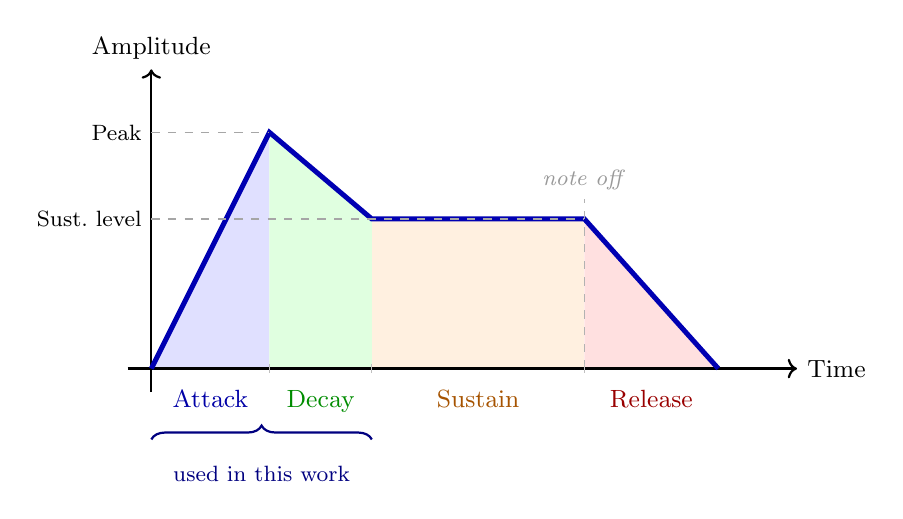
\begin{tikzpicture}
  % Stage shading (drawn first, under envelope line)
  \fill[blue!12]   (0,0) -- (1.5,3.0) -- (1.5,0) -- cycle;
  \fill[green!12]  (1.5,0) -- (1.5,3.0) -- (2.8,1.9) -- (2.8,0) -- cycle;
  \fill[orange!12] (2.8,0) rectangle (5.5,1.9);
  \fill[red!12]    (5.5,0) -- (5.5,1.9) -- (7.2,0) -- cycle;

  % Axes
  \draw[thick, ->] (-0.3,0) -- (8.2,0) node[right, font=\small] {Time};
  \draw[thick, ->] (0,-0.3) -- (0,3.8) node[above, font=\small] {Amplitude};

  % ADSR envelope line
  \draw[blue!70!black, line width=1.8pt]
    (0,0) -- (1.5,3.0) -- (2.8,1.9) -- (5.5,1.9) -- (7.2,0);

  % Dashed reference lines
  \draw[dashed, gray!70] (0,3.0) -- (1.5,3.0);
  \draw[dashed, gray!70] (0,1.9) -- (5.5,1.9);
  \node[left, font=\footnotesize] at (0,3.0) {Peak};
  \node[left, font=\footnotesize] at (0,1.9) {Sust.\ level};

  % Note-off dashed vertical line
  \draw[dashed, gray!60] (5.5,0) -- (5.5,2.15);
  \node[above, font=\footnotesize, gray!80] at (5.5,2.15) {\textit{note off}};

  % Stage boundary ticks on x-axis
  \foreach \x in {1.5, 2.8, 5.5} {
    \draw[gray!50] (\x,0.06) -- (\x,-0.06);
  }

  % Stage labels below x-axis
  \node[below=0.15cm, font=\small, blue!65!black]   at (0.75,0) {Attack};
  \node[below=0.15cm, font=\small, green!55!black]  at (2.15,0) {Decay};
  \node[below=0.15cm, font=\small, orange!65!black] at (4.15,0) {Sustain};
  \node[below=0.15cm, font=\small, red!60!black]    at (6.35,0) {Release};

  % Annotation for stages used in this work
  \draw[decorate, decoration={brace, amplitude=5pt}, thick, blue!50!black]
    (0, -0.9) -- (2.8, -0.9)
    node[midway, below=6pt, font=\footnotesize, blue!50!black] {used in this work};
\end{tikzpicture}
\vspace{0.3cm}
\caption{The ADSR (Attack, Decay, Sustain, Release) envelope shape. A note-on event triggers the Attack; the Decay brings the level down to Sustain, which is held while the key is pressed; Release begins at note-off. Only the Attack and Decay stages are studied here, as all audio clips are fixed 4-second renders with no note-off event. Envelope~1 drives the VCA (amplitude); Envelope~2 drives the filter cutoff, with \texttt{modulation\_1\_amount} controlling the modulation depth.}
\label{fig:adsr}
\end{figure}

\par \vspace{0.3cm}

\noindent \textbf{Voltage-controlled amplifier (VCA).} The VCA multiplies the filtered oscillator signal by the amplitude envelope, imposing the dynamic contour of the sound. Together, the oscillator, filter, and VCA constitute the complete subtractive synthesis signal chain: \textit{Oscillator(s) $\rightarrow$ Filter $\rightarrow$ VCA $\rightarrow$ Effects}. This chain, illustrated in Figure~\ref{fig:synthesis_drivers}, corresponds directly to the four parameter groups studied in this work.

\begin{figure}[H]
\centering
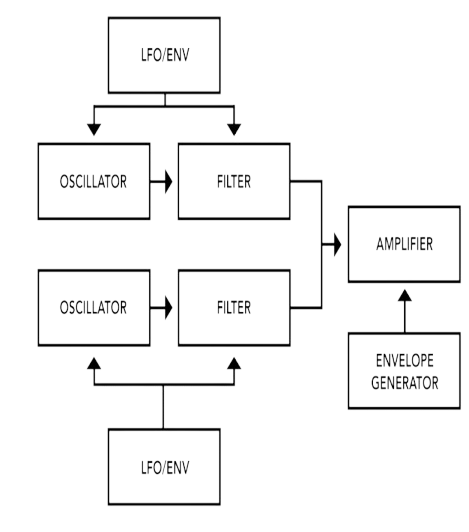
\includegraphics[width=12cm]{images/synthesis_signal_flow.png}
\vspace{0.3cm}
\caption{Signal flow of a subtractive synthesizer, illustrating the key components --- oscillators, filter, envelopes, and effects --- that correspond to the 16 parameters studied in this work \cite{cymatics_subtractive}.}
\label{fig:synthesis_drivers}
\end{figure}

\subsubsubsection{Wavetable Synthesis and the Vital Synthesizer}

\textit{Wavetable synthesis} was introduced by Wolfgang Palm in the PPG Wave synthesizer (1981) and extends the classic oscillator paradigm by replacing a fixed waveform shape with a table of up to 256 single-cycle waveforms. Rather than generating a mathematically defined waveform, the oscillator reads a slice of this table --- the \textit{wave frame} --- and plays it back at the desired pitch. As the wave frame position parameter is swept continuously, the oscillator morphs between successive frames, producing timbral evolution that is not achievable with fixed waveform shapes.

\par \vspace{0.3cm}

\noindent This paradigm has a fundamental implication for inverse synthesis. In FM synthesis, the output spectrum is analytically computable from the operator ratios and modulation indices: a closed-form relationship exists between parameters and spectral content. In subtractive synthesis, the harmonic series of a sawtooth wave is fixed and predictable; the filter shapes it in a mathematically characterizable way. In wavetable synthesis, the spectral content at any wave frame position is determined entirely by the arbitrary waveform data stored in the table. No closed-form relationship exists between the wave frame parameter and the resulting spectrum, and the interaction between wavetable position, unison voice count, inter-voice detune, and the downstream filter produces a high-dimensional, non-linear mapping from parameters to audio that is substantially harder to invert. This opacity is one of the key motivations for the data-driven regression approach taken in this work, and distinguishes Vital from the FM and subtractive synthesizers studied in most prior inverse synthesis research.

\par \vspace{0.3cm}

\noindent Vital is a modern open-source wavetable synthesizer developed by Matt Tytel and released in 2020. It provides two independent wavetable oscillators, each with its own wave frame position, output level, unison voice count, and inter-voice detune. These feed into the classic subtractive signal chain: a resonant filter, amplitude and filter envelope generators, and an effects section including reverb. Unison stacks multiple detuned copies of an oscillator, producing the characteristic width and thickness of contemporary electronic music sounds. The parameter space studied in this work is restricted to 16 controls --- drawn from the oscillators, filter, envelopes, and effects --- inspired by the fixed signal flow of vintage analog synthesizers. Even with modern synthesizers that expose hundreds of parameters, professional producers consistently rely on a small, interpretable subset \cite{cook2002realsound}; restricting the parameter space keeps the regression task tractable while retaining expressive coverage. Vital's open-source nature and programmatic parameter access via the Pedalboard Python library make it uniquely suited for large-scale, reproducible dataset generation, which is central to the methodology described in Section~\ref{sec:methodology}.

\subsubsection{The Inverse Synthesis Problem}

The inverse synthesis problem is formally defined as follows. Let $\mathbf{y}$ denote an audio signal rendered by a synthesizer $\mathcal{S}$ with parameter vector $\mathbf{x} \in [0,1]^N$, such that $\mathbf{y} = \mathcal{S}(\mathbf{x}, p)$, where $p$ is the MIDI pitch at which the note is played. Given $\mathbf{y}$ and $p$, the goal is to recover an estimate $\hat{\mathbf{x}}$ that is as close as possible to the ground-truth $\mathbf{x}$. In this work, $N = 16$.

\par \vspace{0.5cm}

\noindent The problem is inherently challenging for several reasons. First, the mapping from parameters to audio is \textit{highly non-linear}: small changes in certain parameters (e.g., filter resonance near self-oscillation, unison detune at high voice counts) can produce disproportionately large perceptual changes, while large changes in others (e.g., reverb mix at low values) may be nearly imperceptible. Second, the problem is \textit{ill-posed}: multiple distinct parameter configurations can produce perceptually similar or identical sounds. This many-to-one relationship makes the inverse mapping ambiguous and complicates loss function design. Third, parameters are \textit{interdependent}: the perceptual effect of the filter cutoff, for example, depends on the current envelope modulation depth and the oscillator content feeding into it.

\subsubsection{Audio Representations}

The choice of input representation is critical for audio-based regression tasks. Raw waveforms carry full information but are high-dimensional and difficult to process directly with standard architectures. The Short-Time Fourier Transform (STFT) decomposes a signal into a two-dimensional time-frequency representation by applying a windowed DFT at successive frames. The magnitude of the STFT, known as the spectrogram, discards phase information but retains the spectral energy distribution over time, which is sufficient for characterizing synthesis parameters.

\par \vspace{0.5cm}

\noindent The \textit{mel spectrogram} applies a perceptually motivated frequency scale — the mel scale — which compresses high frequencies and expands low frequencies to approximate the resolution of the human auditory system. This representation has become the standard input for audio classification and regression tasks \cite{hershey2017cnn}. A key design trade-off in mel spectrogram computation is the choice of FFT window size and hop length: short windows provide high temporal resolution at the cost of frequency resolution, while long windows provide high frequency resolution at the cost of temporal smearing. For a task spanning parameters as diverse as attack transients (millisecond-scale) and harmonic structure (tens of milliseconds), no single scale is optimal for all parameters. This motivates the multi-scale representation introduced in V2 of this work, where three spectrograms computed at fine, mid, and coarse resolutions are combined into a three-channel input tensor.

\subsection{Literature Review}

\subsubsection{Optimization-Based Inverse Synthesis}

The earliest systematic approaches to synthesizer parameter estimation relied on iterative search. \textit{Genetic Algorithms} (GAs) encode candidate parameter vectors as individuals in a population and evolve them over successive generations using crossover and mutation operators, guided by an audio similarity fitness function \cite{walker2007audiosynthesis}. While GAs are capable of exploring non-convex parameter spaces without gradient information, they require thousands of synthesizer renders per run and do not generalize: a new search must be run from scratch for each target sound. \textit{Hill-climbing} methods — gradient-free local search — share the same limitations and are additionally prone to getting trapped in local optima in high-dimensional, non-convex spaces. These methods have been applied successfully to simple FM and subtractive synthesizers with few parameters, but scale poorly to complex VSTs like Vital.

\subsubsection{Deep Learning for Direct Parameter Regression}

The shift to deep learning reformulated inverse synthesis as a supervised regression problem: a neural network is trained on a large dataset of audio/parameter pairs and learns to predict parameters directly from an audio representation, eliminating the need for iterative synthesis at inference time.

\par \vspace{0.5cm}

\noindent Yee-King et al. \cite{yeeking2018automatic} were among the first to apply deep networks to VST synthesizer programming, demonstrating that multilayer perceptrons trained on spectral features could outperform genetic algorithms on a commercial soft-synth. Barkan et al. \cite{barkan2019inversynth} introduced \textit{InverSynth}, which applied CNNs to the parameter estimation of an FM synthesizer, framing the task as a multi-output regression problem and establishing the use of mel-spectrograms as the primary input representation. InverSynth II \cite{barkan2023inversynth2} extended this work with self-supervised pre-training and inference-time fine-tuning, improving generalization to unseen sounds. Chen et al. \cite{chen2022sound2synth} proposed \textit{Sound2Synth} for FM synthesis parameter estimation using a transformer encoder, demonstrating the applicability of attention-based models to this task.

\par \vspace{0.5cm}

\noindent A common limitation of these works is their focus on FM synthesizers, which have a well-defined and mathematically tractable parameter-to-sound relationship. Wavetable synthesizers like Vital, where the oscillator timbre is determined by an arbitrary wave frame position and the interaction with a filter and modulation chain, present a more complex and less structured mapping that has received comparatively little attention.

\subsubsection{Differentiable Synthesis}

A parallel line of research has explored making the synthesis process itself differentiable, enabling gradient-based optimization of parameters directly in the audio domain. Engel et al. \cite{engel2020ddsp} introduced \textit{DDSP} (Differentiable Digital Signal Processing), a framework that reimplements synthesis operators — harmonic oscillators, filtered noise, reverb — as differentiable modules in a neural network computation graph. This allows training with perceptual audio losses such as the Multi-Scale Spectral (MSS) loss, which measures reconstruction quality at multiple time-frequency resolutions, and has produced compelling results for instrumental sound synthesis and timbre transfer.

\par \vspace{0.5cm}

\noindent Caspe et al. \cite{caspe2022ddx7} extended this paradigm to FM synthesis with \textit{DDX7}, a differentiable implementation of the Yamaha DX7 architecture that enables end-to-end gradient-based sound matching using spectral losses. Uzrad et al. \cite{diffmoog} introduced \textit{DiffMoog}, a differentiable modular synthesizer designed specifically for sound matching, which enables gradient-based optimization of parameters through a differentiable implementation of a Moog-style synthesis chain.

\par \vspace{0.5cm}

\noindent While these approaches are powerful, they share a fundamental requirement: the synthesizer must be re-implemented as a differentiable module. This is feasible for mathematically well-defined synthesizers (FM, additive, physical models) but is not practical for a production VST like Vital, which operates as a non-differentiable black-box plugin. Constructing a differentiable proxy of Vital would require significant additional engineering effort beyond the scope of this work. For this reason, the MSS loss is used in this study as a \textit{post-hoc evaluation metric} only — not as a training objective — and the supervised regression approach over fixed input-output pairs remains the appropriate framework.

\subsubsection{Deep Learning Architectures for Audio}

\subsubsubsection{Convolutional Neural Networks}
CNNs were among the first deep architectures applied to large-scale audio classification, with Hershey et al. \cite{hershey2017cnn} demonstrating strong performance on AudioSet using standard image classification networks applied to log-mel spectrograms. The key insight — that a mel spectrogram can be treated as a 2D image and processed with convolutional feature extractors — established the template for audio deep learning. He et al. \cite{he2016resnet} introduced residual connections (\textit{ResNets}), which enable training of very deep networks by providing gradient shortcuts and form the backbone of the custom CNN baseline used in this work.

\subsubsubsection{Vision Transformers and AST}
Dosovitskiy et al. \cite{dosovitskiy2021vit} introduced the Vision Transformer (ViT), which patches an image into non-overlapping tokens and processes them with a standard Transformer encoder \cite{vaswani2017attention}. Global self-attention allows ViT to capture long-range spatial dependencies that are difficult for local convolutions to model. Gong et al. \cite{gong2021ast} adapted ViT to audio by pre-training on AudioSet spectrograms, yielding the \textit{Audio Spectrogram Transformer} (AST). AST uses a CLS token to produce a global embedding of the spectrogram, making it well-suited as a backbone for regression tasks. The dynamic image size capability of ViT allows it to process non-square spectrograms (such as the $128 \times 224$ inputs used in this work) without requiring architectural changes.

\subsubsubsection{ConvNeXt}
Liu et al. \cite{liu2022convnext} revisited the design space of convolutional networks in light of the advances introduced by vision transformers, systematically modernizing a standard ResNet by adopting inverted bottleneck blocks, depthwise convolution, larger kernels, and GELU activations. The resulting \textit{ConvNeXt} architecture matches or exceeds ViT on standard vision benchmarks while retaining the inductive biases of convolution — translation equivariance and local feature extraction — which are arguably better suited to the structured, locally-correlated spectral patterns of synthesized audio. Pellegrini et al. demonstrated that ConvNeXt pre-trained on ImageNet-22k transfers effectively to audio classification tasks, further motivating its use in this study.

\subsubsection{Sound Matching with Deep Learning: The Primary Baseline}

Bruford et al. \cite{bruford2024ast} applied the Audio Spectrogram Transformer to synthesizer sound matching, training an AST model to predict the parameters of a commercial subtractive synthesizer from audio input. Their work established the strongest prior baseline for the direct regression approach to inverse synthesis using a modern pre-trained backbone. However, several aspects of their setup limit its applicability to the present work: (i) only a single mel-spectrogram scale is used as input; (ii) no pitch information is provided to the model; (iii) only the AST architecture is evaluated, with no comparison to convolutional alternatives; and (iv) the study targets a subtractive synthesizer, whereas this work addresses a wavetable synthesizer whose timbre space is substantially richer. These gaps directly motivate the research questions and contributions of this study.

\subsubsection{Conditioning and Data Augmentation}

\subsubsubsection{FiLM Conditioning}
Perez et al. \cite{perez2018film} introduced \textit{Feature-wise Linear Modulation} (FiLM), a conditioning mechanism in which a conditioning signal (here, MIDI pitch) is passed through a small MLP to predict a scale $\gamma$ and shift $\beta$, which are then applied element-wise to an intermediate feature map: $\tilde{\mathbf{z}} = (1 + \gamma) \odot \mathbf{z} + \beta$. Initializing the FiLM MLP to produce zero output at initialization preserves the identity transform at the start of training, ensuring stable optimization. FiLM provides a principled and expressive alternative to naive concatenation of conditioning features, as it allows the conditioning signal to multiplicatively modulate the feature representation rather than simply augmenting it additively.

\subsubsubsection{SpecAugment}
Park et al. \cite{park2019specaugment} introduced \textit{SpecAugment}, a simple data augmentation strategy for mel spectrograms that applies random masking along the time and frequency axes. By forcing the model to predict from partially occluded representations, SpecAugment acts as a structured regularizer and has been shown to substantially reduce overfitting in audio models. In this work, SpecAugment is applied during V3 training to complement the increased dataset size and further improve generalization.

\subsection{Summary and Research Gap}

Table \ref{tab:litreview_summary} summarizes the key prior works and their relationship to this study.

\begin{table}[H]
\centering
\renewcommand{\arraystretch}{1.3}
\begin{tabular}{p{3.2cm} p{2cm} p{1.8cm} p{1.6cm} p{1.8cm} p{2.5cm}}
\hline
\textbf{Work} & \textbf{Synth Type} & \textbf{Backbone} & \textbf{Pitch Input} & \textbf{Multi-Scale} & \textbf{Dataset Scale} \\
\hline
Yee-King et al. \cite{yeeking2018automatic} & VST & MLP & No & No & Small \\
InverSynth \cite{barkan2019inversynth} & FM & CNN & No & No & Medium \\
Sound2Synth \cite{chen2022sound2synth} & FM & Transformer & No & No & Medium \\
Bruford et al. \cite{bruford2024ast} & Subtractive & AST & No & No & Medium \\
\textbf{This work} & \textbf{Wavetable} & \textbf{CNN / ConvNeXt / AST} & \textbf{Yes (FiLM)} & \textbf{Yes (3-scale)} & \textbf{Large} \\
\hline
\end{tabular}
\vspace{0.3cm}
\caption{Comparison of key prior works in deep learning-based inverse synthesis.}
\label{tab:litreview_summary}
\end{table}

\noindent The table highlights that no prior work has (i) compared ConvNeXt and AST in the same controlled setting, (ii) incorporated explicit pitch conditioning, or (iii) used a multi-scale mel-spectrogram as a multi-channel input for synthesizer parameter estimation. This work addresses all three gaps simultaneously within a unified experimental framework applied to the Vital wavetable synthesizer.

\clearpage
% Include the background and literature and literature review section.

%%%%%%%%%%%%%%%%%%%%%%%%%%%%%%%%%
% Methodology                   %
%%%%%%%%%%%%%%%%%%%%%%%%%%%%%%%%%

\section{METHODOLOGY}
\label{sec:methodology}

\noindent
This section outlines the systematic approach adopted in this study, detailing the research framework, the data generation and processing pipeline, and the tools and technologies employed to achieve the stated objectives.

\subsection{Design Science Research Methodology}

\noindent
Design Science Research (DSR) is a research paradigm whose primary aim is to develop and evaluate purposeful artifacts that address clearly defined practical problems \cite{wieringa2014design}. Unlike observational or explanatory research, DSR is prescriptive: it produces artifacts — models, methods, systems, or frameworks — and evaluates them against the problem context for which they were designed. This makes DSR particularly well-suited to applied computer science and engineering research, where the goal is not only to understand a phenomenon but to build something that improves upon the current state.

\par \vspace{0.3cm}
In this work, the artifact under development is a deep learning framework for synthesizer parameter estimation: a system that takes an audio signal and a MIDI pitch value as inputs and produces a vector of predicted synthesizer parameters as output. The problem context is the inverse synthesis problem — recovering the parameters of a software synthesizer from its audio output — which is a practical challenge faced by sound designers and music producers. DSR is applied here because the work involves designing and iteratively refining a computational artifact, evaluating it against quantitative performance criteria, and drawing design knowledge from the evaluation results to guide subsequent iterations.

\par \vspace{0.3cm}
The iterative nature of DSR aligns naturally with the three-phase experimental structure of this project. Each iteration — V1, V2, and V3 — corresponds to a complete DSR cycle in which a version of the artifact is designed, implemented, and evaluated, with findings feeding directly into the design of the next iteration. This structure ensures that each design decision is motivated by empirical evidence rather than assumption.

\subsection{Design Science Research Iterations}

The DSR process is structured around five interrelated phases, as illustrated in Figure \ref{fig:dsr_cycle}. These phases are not strictly sequential; rather, they form a cycle in which evaluation results inform subsequent problem investigation and solution redesign. The following subsections describe how each phase maps to the work conducted in this study.

\begin{figure}[H]
\centering
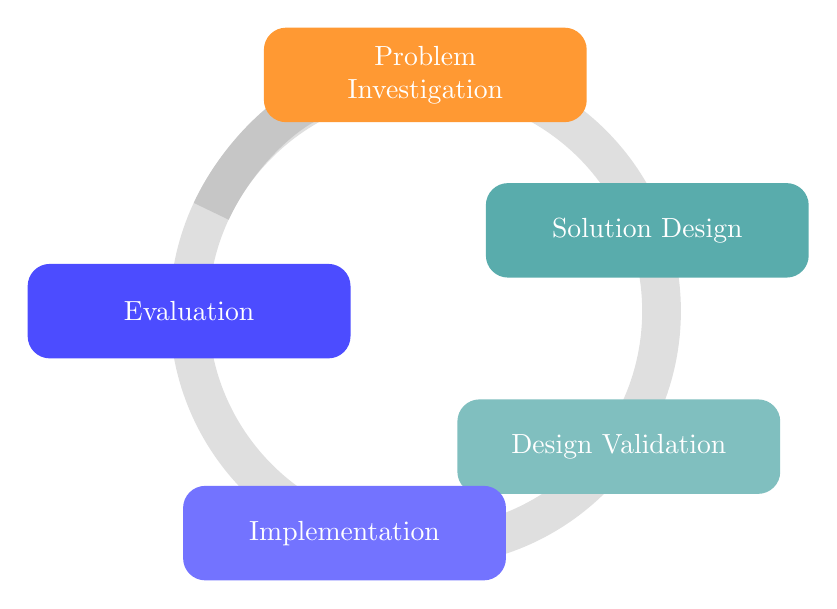
\begin{tikzpicture}[font=\small, >=Stealth]

\draw[line width=14pt, draw=gray!25] (0,0) circle (3.0cm);
\draw[-{Stealth[length=6mm]}, line width=14pt, draw=gray!45]
      (155:3.0cm) arc[start angle=155, end angle=110, radius=3.0cm];

\tikzset{
  dsrbox/.style={rounded corners=8pt, minimum width=4.1cm,
                 minimum height=1.2cm, align=center, font=\normalsize}
}

\node[dsrbox, fill=orange!80, text=white]   (prob)   at (90:3.0cm)   {Problem\\Investigation};
\node[dsrbox, fill=teal!65, text=white]     (design) at (20:3.0cm)   {Solution Design};
\node[dsrbox, fill=teal!50, text=white]     (valid)  at (-35:3.0cm)  {Design Validation};
\node[dsrbox, fill=blue!55, text=white]     (impl)   at (-110:3.0cm) {Implementation};
\node[dsrbox, fill=blue!70, text=white]     (eval)   at (180:3.0cm)  {Evaluation};

\end{tikzpicture}
\vspace{0.4cm}
\caption{Design Science Research cycle with the five phases applied in this study.}
\label{fig:dsr_cycle}
\end{figure}

\noindent Table~\ref{tab:dsr_mapping} maps each DSR phase to the specific activities carried out in this study, the artifact or output produced, and the section in which it is reported.

\begin{table}[H]
\centering
\renewcommand{\arraystretch}{1.4}
\begin{tabular}{p{2.8cm} p{4.8cm} p{3.6cm} p{2.0cm}}
\hline
\textbf{DSR Phase} & \textbf{Activity in this study} & \textbf{Output} & \textbf{Reported in} \\
\hline
Problem Investigation  & Literature review; gap analysis; formulation of research questions RQ1--RQ3 & Research questions; literature gap table & Sections 1, 2 \\
Solution Design        & Dataset strategy; input representation; architecture and training objective design & V1, V2, V3 design specifications & Section 4 \\
Design Validation      & Architecture correctness checks; V2 controlled ablation study isolating each component & Per-component MAE impact; ablation results & Sections 4, 5 \\
Solution Implementation & V1$\to$V2$\to$V3 model training across cross-validation splits & Trained model checkpoints & Section 4 \\
Solution Evaluation    & MAE and MSS evaluation on held-out test sets; per-parameter breakdown; architecture comparison & Results tables; analysis & Section 5 \\
\hline
\end{tabular}
\vspace{0.3cm}
\caption{Mapping of the five DSR phases to project activities, outputs, and report sections.}
\label{tab:dsr_mapping}
\end{table}

\subsubsection{Problem Investigation}

The problem investigation phase begins with a thorough analysis of the existing literature on inverse synthesis, audio deep learning, and synthesizer parameter estimation. This review, presented in Section 2, revealed several gaps in the current state of the art: (i) no prior work has applied deep learning-based parameter estimation to a modern wavetable synthesizer such as Vital; (ii) existing approaches rely on a single mel-spectrogram scale, ignoring the complementary information available at different time-frequency resolutions; (iii) no prior work incorporates explicit pitch conditioning to disentangle timbral features from the fundamental frequency; and (iv) the Audio Spectrogram Transformer and ConvNeXt architectures have never been directly compared in the context of synthesizer sound matching.

\par \vspace{0.3cm}
These gaps, combined with the practical motivation of building a tool useful to sound designers and producers, constitute the ``wicked problem'' that drives this research: a high-dimensional, non-linear, ill-posed inverse mapping whose difficulty is compounded by parameter interdependence, timbral ambiguity, and the non-differentiable nature of the target synthesizer. The three research questions formulated in Section 1 directly address the identified gaps and guide the design effort.

\subsubsection{Solution Design}

The solution design phase translates the problem formulation into a concrete artifact specification. Three core design decisions structure this phase.

\par \vspace{0.3cm}
First, the \textbf{dataset design}: rather than sampling parameters uniformly at random — which would produce mostly silent or musically incoherent sounds — a timbre-constrained generation strategy is devised. Parameters are sampled within musically meaningful sub-ranges defined for five timbre categories (bass, lead, pad, percussion, and random), and audio is rendered programmatically via the Pedalboard library driving Vital. The parameter space is restricted to 16 controls inspired by the canonical analog signal chain of the Minimoog and Prophet-5.

\par \vspace{0.3cm}
Second, the \textbf{input representation design}: a multi-scale mel spectrogram is proposed as a three-channel input tensor, combining fine, mid, and coarse time-frequency resolutions to provide the model with complementary views of each audio clip. This design directly addresses the resolution trade-off inherent in single-scale representations.

\par \vspace{0.3cm}
Third, the \textbf{architecture design}: three backbone families are selected for comparison — a custom residual CNN, a pre-trained ConvNeXt, and a pre-trained Audio Spectrogram Transformer — each augmented with a FiLM-based pitch conditioning branch and a grouped prediction head that assigns a dedicated sub-MLP to each semantically coherent parameter group.

\subsubsection{Design Validation}

Design validation is carried out through a systematic ablation study in the V2 iteration. Each architectural innovation introduced in V2 — multi-scale input, FiLM pitch conditioning, and the grouped prediction head — is evaluated in isolation by training variants in which only one component is removed or simplified at a time, while all other factors are held constant. This controlled approach ensures that performance differences are attributable to the specific component under test, rather than to confounding factors. The results of this ablation study, reported in Section 5, provide the empirical basis for the design choices carried forward into V3.

\subsubsection{Solution Implementation}

Implementation proceeds across three successive iterations, each building on the validated design of its predecessor.

\par \vspace{0.3cm}
\textbf{V1} establishes the baseline: a dataset of single-scale mel spectrograms is generated, and the three model families are trained and compared under identical conditions. The optional sinusoidal pitch embedding branch is evaluated as a simple concatenation-based conditioning mechanism.

\par \vspace{0.3cm}
\textbf{V2} implements all three architectural innovations simultaneously: multi-scale mel input, FiLM pitch conditioning, and the grouped prediction head with weighted loss. A full ablation suite is trained alongside the main models to validate each component.

\par \vspace{0.3cm}
\textbf{V3} addresses the key failure mode identified in V2 — the ineffectiveness of pitch conditioning when each preset is rendered at only a single MIDI pitch. By re-rendering every preset at three distinct MIDI notes per timbre, the dataset grows substantially, and the model is now exposed to the same parameter vector at different spectral positions, providing a meaningful conditioning signal for the FiLM branch. SpecAugment regularization is also introduced at this stage.

\subsubsection{Solution Evaluation}

Evaluation is conducted at two levels. The primary metric is the Mean Absolute Error (MAE) computed in the normalized $[0,1]$ parameter space, reported as mean $\pm$ standard deviation across five cross-validation splits to ensure statistical robustness. Per-parameter MAE is additionally reported to identify which synthesis controls are well-predicted and which remain structurally ambiguous. For V2 and V3, a Multi-Scale Spectral (MSS) loss is computed on a held-out test subset by re-rendering the predicted parameters through Vital and measuring the spectral distance between the original and reconstructed audio, providing a perceptual evaluation complementary to the parameter-space MAE.

% ─────────────────────────────────────────────────────────
\subsection{Data Generation Pipeline}

The data generation pipeline transforms raw synthesizer parameter configurations into a normalized, split dataset ready for model training. It consists of six sequential steps, illustrated in Figure~\ref{fig:pipeline}. Each step is designed to be checkpoint-aware and resumable, as the full pipeline involves several hours of audio rendering and processing.

\begin{figure}[H]
\centering
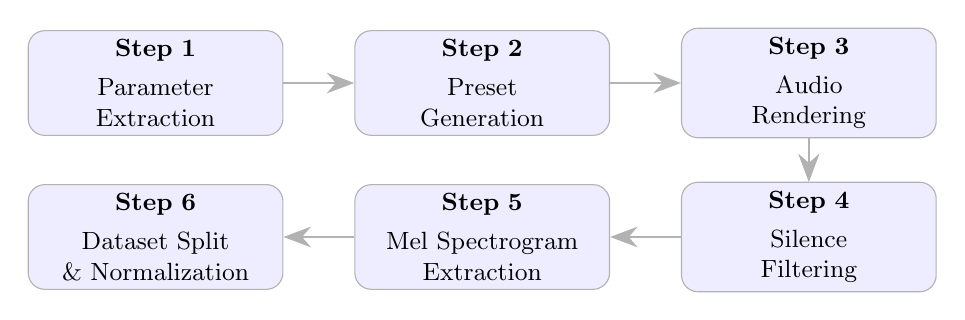
\begin{tikzpicture}[
  node distance=0.55cm and 0.9cm,
  box/.style={rectangle, rounded corners=6pt, draw=gray!60, fill=blue!7,
              text width=3.0cm, align=center, minimum height=1.3cm, font=\small},
  arrow/.style={-{Stealth[length=3.5mm]}, thick, gray!60}
]

% Row 1
\node[box] (s1) {\textbf{Step 1}\\[3pt]Parameter\\Extraction};
\node[box, right=of s1] (s2) {\textbf{Step 2}\\[3pt]Preset\\Generation};
\node[box, right=of s2] (s3) {\textbf{Step 3}\\[3pt]Audio\\Rendering};

% Row 2 (right to left below row 1)
\node[box, below=of s3] (s4) {\textbf{Step 4}\\[3pt]Silence\\Filtering};
\node[box, left=of s4]  (s5) {\textbf{Step 5}\\[3pt]Mel Spectrogram\\Extraction};
\node[box, left=of s5]  (s6) {\textbf{Step 6}\\[3pt]Dataset Split\\\& Normalization};

% Arrows
\draw[arrow] (s1) -- (s2);
\draw[arrow] (s2) -- (s3);
\draw[arrow] (s3) -- (s4);
\draw[arrow] (s4) -- (s5);
\draw[arrow] (s5) -- (s6);

% Corner connector
\draw[arrow] (s3.south) -- (s4.north);

\end{tikzpicture}
\vspace{0.3cm}
\caption{The six-step data generation pipeline, from parameter extraction to normalized dataset splits.}
\label{fig:pipeline}
\end{figure}

% ─────────────────────────────────────────────────────────
\subsubsection{Step 1: Parameter Extraction from Vital}

All 16 target parameters are enumerated programmatically from Vital via the Pedalboard Python library, which exposes the synthesizer's internal parameter table. For each parameter, the extraction records its name, internal plugin index, valid range $[x^{\min}_k,\, x^{\max}_k]$, and discretization information where applicable. Seven parameters — the four envelope times, the filter cutoff, the unison voice count, and the oscillator 2 transpose — are internally quantized by Vital to a finite set of valid discrete values. During preset generation, any continuously sampled value for these parameters is snapped to the nearest valid discrete point. The extracted ranges and discrete value tables are stored as JSON reference files and used throughout the pipeline to ensure that all generated presets are valid within Vital's internal representation. Table~\ref{tab:parameters} provides the complete listing of all 16 parameters in their prediction order, together with their group assignment, the normalization applied to raw Vital values before min-max scaling to $[0,1]$, whether the parameter is internally discretized by Vital, and the loss weight assigned to each group during training (see Equation~\ref{eq:weighted_loss} in Section 4).

\begin{table}[H]
\centering
\renewcommand{\arraystretch}{1.35}
\begin{tabular}{clp{2.2cm}p{2.4cm}cc}
\hline
\textbf{\#} & \textbf{Parameter} & \textbf{Group} & \textbf{Normalisation} & \textbf{Discrete} & \textbf{Loss wt.} \\
\hline
0  & \texttt{osc1\_wave\_frame}    & Oscillator & Linear        & ---  & $2\times$ \\
1  & \texttt{osc1\_level}          & Oscillator & Linear        & ---  & $2\times$ \\
2  & \texttt{osc1\_unison\_voices} & Oscillator & Linear        & Yes  & $2\times$ \\
3  & \texttt{osc1\_unison\_detune} & Oscillator & Linear        & ---  & $2\times$ \\
4  & \texttt{osc2\_wave\_frame}    & Oscillator & Linear        & ---  & $2\times$ \\
5  & \texttt{osc2\_level}          & Oscillator & Linear        & ---  & $2\times$ \\
6  & \texttt{osc2\_transpose}      & Oscillator & Linear        & Yes  & $2\times$ \\
\hline
7  & \texttt{env1\_attack}         & Envelope   & $\log_{10}$   & Yes  & $1\times$ \\
8  & \texttt{env1\_decay}          & Envelope   & $\log_{10}$   & Yes  & $1\times$ \\
9  & \texttt{env2\_attack}         & Envelope   & $\log_{10}$   & Yes  & $1\times$ \\
10 & \texttt{env2\_decay}          & Envelope   & $\log_{10}$   & Yes  & $1\times$ \\
\hline
11 & \texttt{filter1\_cutoff}      & Filter     & $\log_{10}$   & Yes  & $1\times$ \\
12 & \texttt{filter1\_resonance}   & Filter     & Linear        & ---  & $1\times$ \\
\hline
13 & \texttt{sample\_level}        & Misc       & Linear        & ---  & $1\times$ \\
14 & \texttt{mod1\_amount}         & Misc       & Linear        & ---  & $1\times$ \\
15 & \texttt{reverb\_mix}          & Misc       & Linear        & ---  & $1\times$ \\
\hline
\end{tabular}
\vspace{0.3cm}
\caption{All 16 synthesizer parameters in prediction order (index 0--15). \textit{Normalisation} is the transform applied to raw Vital values before min-max scaling to $[0,1]$: envelope times and filter cutoff span several orders of magnitude and are $\log_{10}$-transformed first. \textit{Discrete} indicates parameters that Vital internally quantizes to a finite grid; sampled values are snapped to the nearest valid point during preset generation. \textit{Loss wt.} is the group weighting applied in the training objective. Sustain and release are excluded as both stages are unobservable in a fixed 4-second render with no note-off event.}
\label{tab:parameters}
\end{table}

% ─────────────────────────────────────────────────────────
\subsubsection{Step 2: Timbre-Constrained Preset Generation}

A naive uniform sampling of the 16-dimensional parameter space produces predominantly silent, extremely bright, or otherwise pathological sounds of little musical relevance. To ensure that the dataset covers a representative range of practically meaningful sounds, a \textit{timbre-constrained} generation strategy is employed. Five timbre categories are defined, each associated with a set of parameter sub-ranges that constrain the sampling to musically coherent regions of the parameter space. The categories and their MIDI pitch ranges are summarized in Table~\ref{tab:timbre_categories}.

\begin{table}[H]
\centering
\renewcommand{\arraystretch}{1.3}
\begin{tabular}{lcccc}
\hline
\textbf{Timbre} & \textbf{Min MIDI} & \textbf{Max MIDI} & \textbf{Notes} & \textbf{Presets} \\
\hline
bass   & C0 (12) & C3 (48) & Low register, slow envelope      & 6{,}000  \\
lead   & C3 (48) & C6 (84) & Mid-high register, bright timbre  & 6{,}000  \\
pad    & C2 (36) & C5 (72) & Sustained, slow attack            & 6{,}000  \\
percs  & C1 (24) & C6 (84) & Short attack, noise-heavy         & 6{,}000  \\
random & C0 (12) & C6 (84) & Unconstrained full range          & 20{,}000 \\
\hline
\textbf{Total} & & & & \textbf{44{,}000} \\
\hline
\end{tabular}
\vspace{0.3cm}
\caption{Timbre categories used for preset generation, with their MIDI pitch ranges and preset counts.}
\label{tab:timbre_categories}
\end{table}

\noindent For each timbre, a JSON range file defines per-parameter minimum and maximum bounds that enforce the target timbre. For example, the \texttt{percs} category enforces a very short amplitude attack ($\leq 10$ ms), a moderate decay range, and a high noise/sample oscillator level, ensuring that any random draw within those bounds produces a percussive-sounding result. Each preset is stored as a record in a per-timbre JSONL file, with checkpoint-aware deduplication allowing interrupted generation runs to be safely resumed.

% ─────────────────────────────────────────────────────────
\subsubsection{Step 3: Audio Rendering}

Each preset is rendered to a 44.1 kHz mono WAV file via Pedalboard, which loads Vital as a VST3 plugin, sets all 16 parameters programmatically, and triggers a MIDI note-on event without a corresponding note-off. The clip duration is fixed at 4 seconds. The absence of a note-off event means that the release stage of the amplitude envelope is never triggered, which is why release is excluded from the 16 studied parameters. The sustain stage is similarly excluded, as the envelope decay is set long enough relative to the 4-second clip to produce effectively sustained sounds without requiring an explicit sustain parameter.

\par \vspace{0.3cm}
In V1 and V2, each preset is rendered at a single MIDI pitch sampled uniformly from the timbre's valid range. In V3, each preset is rendered at three fixed MIDI pitches chosen to cover the low, mid, and high registers of the timbre's range, expanding the dataset approximately three-fold. A SHA-256 hash of the parameter vector and MIDI pitch is used to track already-rendered presets, enabling safe resumption of interrupted runs. Rendered audio paths and ground-truth parameters are written to a combined JSONL file with one record per clip.

% ─────────────────────────────────────────────────────────
\subsubsection{Step 4: Silence Filtering}

Certain extreme parameter combinations cause Vital to produce no audible output — for example, when both oscillators are muted and the sample level is zero. These silent clips are detected and removed using a hybrid energy-based rule applied to each rendered WAV file.

\par \vspace{0.3cm}
The audio signal $x(n)$ is divided into short frames of length $L$ with hop $H$. The RMS energy of the $i$-th frame is computed as:

\begin{equation}
E_i = \sqrt{\frac{1}{L} \sum_{n=0}^{L-1} x^2(iH + n)}
\label{eq:rms}
\end{equation}

\noindent and converted to decibels:

\begin{equation}
E_i^{\text{dB}} = 20 \cdot \log_{10}(E_i + \epsilon)
\label{eq:rms_db}
\end{equation}

\noindent where $\epsilon$ is a small floor value to avoid $\log(0)$. Two detection rules are then applied:

\begin{equation}
R = \frac{1}{N_f} \sum_{i=1}^{N_f} \mathbf{1}\!\left[E_i^{\text{dB}} > \theta_{\text{rms}}\right]
\label{eq:active_ratio}
\end{equation}

\begin{equation}
P^{\text{dB}} = 20 \cdot \log_{10}\!\left(\max_{n}\,|x(n)|\right)
\label{eq:peak_db}
\end{equation}

\noindent where $R$ is the \textit{active ratio} — the fraction of frames exceeding the RMS threshold $\theta_{\text{rms}}$ — and $P^{\text{dB}}$ is the peak amplitude in decibels. A clip is retained if either condition is satisfied:

\begin{equation}
\text{keep} \;\Leftrightarrow\; \left(R > \rho_{\min}\right) \;\vee\; \left(P^{\text{dB}} > \theta_{\text{peak}}\right)
\label{eq:keep_rule}
\end{equation}

\noindent The logical OR ensures that transient-heavy sounds such as percussions — which concentrate energy in a small number of frames and would fail the active ratio rule alone — are not incorrectly discarded. The per-timbre thresholds are given in Table~\ref{tab:silence_thresholds}.

\begin{table}[H]
\centering
\renewcommand{\arraystretch}{1.3}
\begin{tabular}{lccc}
\hline
\textbf{Timbre} & $\boldsymbol{\theta_{\text{rms}}}$ \textbf{(dB)} & $\boldsymbol{\rho_{\min}}$ & $\boldsymbol{\theta_{\text{peak}}}$ \textbf{(dB)} \\
\hline
bass   & $-50.0$ & $0.020$ & $-28.0$ \\
lead   & $-50.0$ & $0.020$ & $-28.0$ \\
pad    & $-55.0$ & $0.015$ & $-30.0$ \\
percs  & $-50.0$ & $0.002$ & $-30.0$ \\
random & $-50.0$ & $0.010$ & $-30.0$ \\
\hline
\end{tabular}
\vspace{0.3cm}
\caption{Per-timbre silence detection thresholds used in the hybrid RMS filtering step.}
\label{tab:silence_thresholds}
\end{table}

% ─────────────────────────────────────────────────────────
\subsubsection{Step 5: Mel Spectrogram Extraction}

Each surviving audio clip is converted to a mel spectrogram representation. Given the discrete-time audio signal $x(n)$ at sample rate $f_s = 44{,}100$ Hz, the Short-Time Fourier Transform (STFT) is first computed as:

\begin{equation}
X(t, f) = \sum_{n} x(n)\, w(n - tH)\, e^{-j2\pi fn/N}
\label{eq:stft}
\end{equation}

\noindent where $w$ is a Hann window of length $N$ (the FFT size), $H$ is the hop length, and $t$ indexes time frames. The power spectrogram is then obtained as:

\begin{equation}
P(t, f) = |X(t, f)|^2
\label{eq:power_spec}
\end{equation}

\noindent A bank of $M = 128$ triangular mel filters $\{H_m(f)\}_{m=1}^{M}$, spaced according to the mel scale between $f_{\min} = 20$ Hz and $f_{\max} = 12{,}000$ Hz, is applied to yield the mel spectrogram:

\begin{equation}
S(t, m) = 10 \cdot \log_{10}\!\left(\sum_{f} H_m(f)\, P(t, f) + \epsilon\right)
\label{eq:mel}
\end{equation}

\noindent This produces a $128 \times T$ matrix, where $T$ is the number of time frames.

\par \vspace{0.3cm}
\noindent \textbf{V1 — Single-Scale.} A single mel spectrogram is extracted using the mid-scale FFT configuration (Table~\ref{tab:mel_scales}) and stored as a \texttt{.npy} file.

\par \vspace{0.3cm}
\noindent \textbf{V2 — Multi-Scale.} Three mel spectrograms are extracted per clip at fine, mid, and coarse resolutions. As the FFT window size increases, spectral resolution improves at the cost of temporal resolution, and vice versa. Table~\ref{tab:mel_scales} lists the parameters of each scale and the type of information each captures.

\begin{table}[H]
\centering
\renewcommand{\arraystretch}{1.3}
\begin{tabular}{lcccp{4.5cm}}
\hline
\textbf{Scale} & \textbf{n\_fft} & \textbf{Hop} & \textbf{Raw Frames ($T$)} & \textbf{Captures} \\
\hline
Fine   & 512   & 128   & $\approx$1{,}378 & Attack transients, onset details \\
Mid    & 2{,}048 & 512   & $\approx$345     & Timbral balance, envelope shape  \\
Coarse & 8{,}192 & 2{,}048 & $\approx$87      & Harmonic structure, pitch content \\
\hline
\multicolumn{5}{l}{\small All scales: 128 mel bins, $f_{\min}=20$ Hz, $f_{\max}=12{,}000$ Hz, $f_s=44{,}100$ Hz.}\\
\multicolumn{5}{l}{\small All inputs padded or truncated to 224 time frames for ConvNeXt/AST.}\\
\hline
\end{tabular}
\vspace{0.3cm}
\caption{Multi-scale mel spectrogram configurations used in V2 and V3.}
\label{tab:mel_scales}
\end{table}

\noindent The three spectrograms are stacked along the channel dimension to form a three-channel input tensor of shape $(3, 128, 224)$, as illustrated in Figure~\ref{fig:multiscale_stack}. This is directly compatible with the three-channel (RGB) first-layer weight initialization of ConvNeXt and ViT backbones.

\begin{figure}[H]
\centering
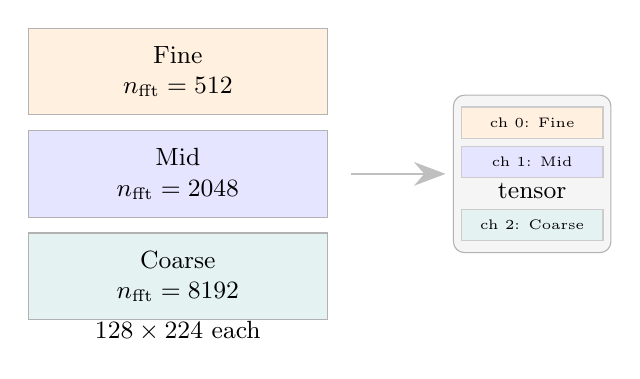
\begin{tikzpicture}[
  spec/.style={draw=gray!60, fill=blue!6, minimum width=3.8cm, minimum height=1.1cm,
               align=center, font=\small},
  label/.style={font=\small, align=center},
  arrow/.style={-{Stealth[length=4mm]}, thick, gray!50}
]

% Three spectrogram slabs
\node[spec, fill=orange!12] (fine)   at (0, 2.6) {Fine\\$n_{\text{fft}}=512$};
\node[spec, fill=blue!10]   (mid)    at (0, 1.3) {Mid\\$n_{\text{fft}}=2048$};
\node[spec, fill=teal!10]   (coarse) at (0, 0.0) {Coarse\\$n_{\text{fft}}=8192$};

\node[label] at (0, -0.7) {$128\times224$ each};

% Brace / arrow
\draw[arrow] (2.2, 1.3) -- (3.4, 1.3);

% Stacked tensor box
\draw[fill=gray!8, draw=gray!60, rounded corners=4pt]
  (3.5, 0.3) rectangle (5.5, 2.3);
\node[font=\small, align=center] at (4.5, 1.3)
  {$(3, 128, 224)$\\\small tensor};

% Channel labels inside
\draw[fill=orange!12, draw=gray!40] (3.6, 1.75) rectangle (5.4, 2.15);
\draw[fill=blue!10,   draw=gray!40] (3.6, 1.25) rectangle (5.4, 1.65);
\draw[fill=teal!10,   draw=gray!40] (3.6, 0.45) rectangle (5.4, 0.85);
\node[font=\tiny] at (4.5, 1.95) {ch 0: Fine};
\node[font=\tiny] at (4.5, 1.45) {ch 1: Mid};
\node[font=\tiny] at (4.5, 0.65) {ch 2: Coarse};

\end{tikzpicture}
\vspace{0.3cm}
\caption{Three mel spectrograms at fine, mid, and coarse resolutions stacked into a single three-channel input tensor of shape $(3, 128, 224)$.}
\label{fig:multiscale_stack}
\end{figure}

% ─────────────────────────────────────────────────────────
\subsubsection{Step 6: Dataset Splitting and Normalization}

\subsubsubsection{Stratified Split}
To ensure that each data split contains a representative distribution of both timbre categories and pitch registers, a stratified splitting strategy is employed. Each sample is assigned a bucket key:

\begin{equation}
\text{bucket} = \left(\text{timbre},\; \left\lfloor \frac{\text{midi\_note}}{12} \right\rfloor\right)
\label{eq:bucket}
\end{equation}

\noindent Within each bucket, samples are deterministically shuffled using a seeded random number generator and then divided in an 80 / 10 / 10 ratio into training, validation, and test sets. Five independent splits are generated using different random seeds, producing five-fold cross-validation splits for robust evaluation. In V3, the split is performed at the \textit{preset level}: all three pitch renderings of the same preset are assigned to the same split, preventing any form of data leakage between training and evaluation sets.

\subsubsubsection{Normalization}
Three normalization schemes are applied, each fitted exclusively on training data and applied identically to validation and test sets to prevent data leakage.

\par \vspace{0.3cm}
\textit{Mel spectrograms} are Z-score normalized per scale:

\begin{equation}
\hat{S}(t, m) = \frac{S(t, m) - \mu_{\text{train}}}{\sigma_{\text{train}}}
\label{eq:zscore}
\end{equation}

\noindent \textit{Synthesizer parameters} are min-max normalized per parameter to $[0, 1]$:

\begin{equation}
\hat{x}_k = \frac{x_k - x_k^{\min}}{x_k^{\max} - x_k^{\min}}, \quad k = 1, \ldots, 16
\label{eq:minmax}
\end{equation}

\noindent \textit{MIDI pitch} is normalized to $[0, 1]$ using the fixed global range $[12, 84]$:

\begin{equation}
p = \frac{\text{midi\_note} - 12}{84 - 12}
\label{eq:pitch_norm}
\end{equation}

\noindent This normalized scalar $p \in [0, 1]$ is then passed through a sinusoidal embedding to produce a rich 128-dimensional Fourier feature vector:

\begin{equation}
\boldsymbol{\phi}(p) = \left[\sin(\omega_0 p),\, \cos(\omega_0 p),\, \sin(\omega_1 p),\, \cos(\omega_1 p),\, \ldots,\, \sin(\omega_{63} p),\, \cos(\omega_{63} p)\right]
\label{eq:sinusoidal}
\end{equation}

\noindent where the frequencies $\omega_k = 2^k \cdot \pi$ are log-spaced from $\omega_0 = \pi$ to $\omega_{63} = 2^{63}\pi$. This avoids float32 overflow from naive power scaling and provides the model with a dense, multi-frequency representation of the pitch scalar. The final dataset sizes after filtering and splitting are summarized in Table~\ref{tab:dataset_sizes}.

\begin{table}[H]
\centering
\renewcommand{\arraystretch}{1.3}
\begin{tabular}{lcccccc}
\hline
\textbf{Version} & \textbf{Presets} & \textbf{Pitches / Preset} & \textbf{Total Samples} & \textbf{Train} & \textbf{Val} & \textbf{Test} \\
\hline
V1 / V2 & $\approx$42{,}520 & 1 & $\approx$42{,}520 & $\approx$34{,}016 & $\approx$4{,}252 & $\approx$4{,}252 \\
V3      & $\approx$42{,}520 & 3 & $\approx$127{,}000 & $\approx$101{,}600 & $\approx$12{,}700 & $\approx$12{,}700 \\
\hline
\end{tabular}
\vspace{0.3cm}
\caption{Dataset sizes across experimental versions. V3 splits are performed at preset level to prevent leakage.}
\label{tab:dataset_sizes}
\end{table}

% ─────────────────────────────────────────────────────────
\subsection{Technologies}

Table~\ref{tab:technologies} lists the core tools and libraries used across the data generation, model training, and evaluation stages of this project.

\begin{table}[H]
\centering
\renewcommand{\arraystretch}{1.3}
\begin{tabular}{p{3.2cm} p{10cm}}
\hline
\textbf{Tool / Library} & \textbf{Role} \\
\hline
Vital                   & Open-source wavetable VST3 synthesizer; audio generation engine and source of ground-truth parameters \\
Pedalboard (Spotify)    & Python VST plugin host; used to load Vital, set parameters programmatically, and render audio clips \\
Librosa                 & Audio analysis: mel spectrogram extraction, RMS energy computation, spectral descriptor calculation \\
SoundFile               & Low-level WAV file reading and writing \\
NumPy                   & Numerical operations, array manipulation, and preset JSONL handling \\
PyTorch                 & Model definition, training loop, loss computation, and inference \\
timm                    & Pre-trained vision model zoo; provides ConvNeXt and ViT/AST backbones with ImageNet-22k weights \\
Python 3.10             & Full pipeline orchestration across all six data generation steps and model training \\
CUDA / AMP              & GPU-accelerated training on NVIDIA RTX 4090 with automatic mixed precision \\
\hline
\end{tabular}
\vspace{0.3cm}
\caption{Tools and libraries used in the data generation, training, and evaluation pipeline.}
\label{tab:technologies}
\end{table}


\clearpage
% Include the methodology sections.

%%%%%%%%%%%%%%%%%%%%%%%%%%%%%%%%%
% Iterations                    %
%%%%%%%%%%%%%%%%%%%%%%%%%%%%%%%%%

\section{ITERATIONS}
\label{sec:iterations}

\noindent
The development of the synthesizer parameter estimation system followed a systematic iteration-based process guided by the Design Science Research framework introduced in Section~\ref{sec:methodology}. Three successive iterations — V1, V2, and V3 — were conducted, each corresponding to a complete DSR cycle in which a version of the artifact was designed, implemented, and evaluated, with empirical findings feeding directly into the design of the subsequent iteration. Each iteration introduces a distinct set of architectural or data-regime improvements motivated by the limitations uncovered in the preceding cycle.

% ─────────────────────────────────────────────────────────
\subsection{Data Generation Pipeline}

The data generation pipeline transforms raw synthesizer parameter configurations into a normalized, split dataset ready for model training. It consists of six sequential steps, illustrated in Figure~\ref{fig:pipeline}. Each step is designed to be checkpoint-aware and resumable, as the full pipeline involves several hours of audio rendering and processing.

\begin{figure}[H]
\centering
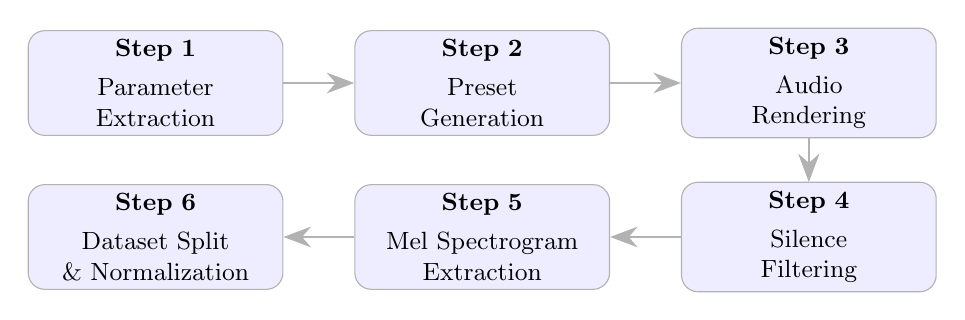
\begin{tikzpicture}[
  node distance=0.55cm and 0.9cm,
  box/.style={rectangle, rounded corners=6pt, draw=gray!60, fill=blue!7,
              text width=3.0cm, align=center, minimum height=1.3cm, font=\small},
  arrow/.style={-{Stealth[length=3.5mm]}, thick, gray!60}
]

% Row 1
\node[box] (s1) {\textbf{Step 1}\\[3pt]Parameter\\Extraction};
\node[box, right=of s1] (s2) {\textbf{Step 2}\\[3pt]Preset\\Generation};
\node[box, right=of s2] (s3) {\textbf{Step 3}\\[3pt]Audio\\Rendering};

% Row 2 (right to left below row 1)
\node[box, below=of s3] (s4) {\textbf{Step 4}\\[3pt]Silence\\Filtering};
\node[box, left=of s4]  (s5) {\textbf{Step 5}\\[3pt]Mel Spectrogram\\Extraction};
\node[box, left=of s5]  (s6) {\textbf{Step 6}\\[3pt]Dataset Split\\\& Normalization};

% Arrows
\draw[arrow] (s1) -- (s2);
\draw[arrow] (s2) -- (s3);
\draw[arrow] (s3) -- (s4);
\draw[arrow] (s4) -- (s5);
\draw[arrow] (s5) -- (s6);

% Corner connector
\draw[arrow] (s3.south) -- (s4.north);

\end{tikzpicture}
\vspace{0.3cm}
\caption{The six-step data generation pipeline, from parameter extraction to normalized dataset splits.}
\label{fig:pipeline}
\end{figure}

% ─────────────────────────────────────────────────────────
\subsubsection{Step 1: Parameter Extraction from Vital}

All 16 target parameters are enumerated programmatically from Vital via the Pedalboard Python library, which exposes the synthesizer's internal parameter table. For each parameter, the extraction records its name, internal plugin index, valid range $[x^{\min}_k,\, x^{\max}_k]$, and discretization information where applicable. While all parameters are exposed with continuous-looking ranges, Vital internally quantizes seven of them to a finite set of valid discrete values. Although these parameters may appear continuous from outside the synthesizer, Vital's internal implementation restricts them to specific grids:

\begin{itemize}
    \item \textbf{Envelope times} (\texttt{env1\_attack}, \texttt{env1\_decay}, \texttt{env2\_attack}, \texttt{env2\_decay}): Despite being specified in seconds over a wide range, all four envelope times are mapped to 1{,}001 discrete steps on a logarithmic time grid. This quantization reflects the resolution of Vital's internal envelope generator, meaning that many nominally distinct floating-point time values collapse to the same rendered behaviour.

    \item \textbf{Filter cutoff} (\texttt{filter1\_cutoff}): Expressed in semitones over a broad pitch range, the filter cutoff is internally quantized to 1{,}001 discrete frequency values. Although the parameter appears continuous, Vital's filter implementation operates on a fixed frequency grid of that resolution.

    \item \textbf{Unison voice count} (\texttt{osc1\_unison\_voices}): Controls how many detuned copies of oscillator 1 are layered to produce a thicker sound. This parameter is inherently discrete, as a fractional number of voices has no physical meaning within the synthesizer engine.

    \item \textbf{Oscillator 2 transpose} (\texttt{osc2\_transpose}): Sets the pitch offset of oscillator 2 relative to the played note. This parameter is inherently discrete by musical convention, taking only integer semitone values.
\end{itemize}

The extracted ranges and discrete value tables are stored as JavaScript Object Notation (JSON) reference files and used throughout the pipeline. Table~\ref{tab:parameters} lists all 16 parameters in their prediction order, along with their discrete status and a brief description.

\begin{table}[H]
\centering
\renewcommand{\arraystretch}{1.35}
\begin{tabular}{clcp{6.5cm}}
\hline
\textbf{\#} & \textbf{Parameter} & \textbf{Discrete} & \textbf{Description} \\
\hline
0  & \texttt{osc1\_wave\_frame}    & ---  & Wavetable position of oscillator 1, controlling the spectral shape of its output waveform. \\
1  & \texttt{osc1\_level}          & ---  & Output amplitude of oscillator 1. \\
2  & \texttt{osc1\_unison\_voices} & Yes  & Number of detuned voices layered by oscillator 1 to produce a thicker sound. \\
3  & \texttt{osc1\_unison\_detune} & ---  & Pitch spread between the unison voices of oscillator 1. \\
4  & \texttt{osc2\_wave\_frame}    & ---  & Wavetable position of oscillator 2, controlling its spectral character. \\
5  & \texttt{osc2\_level}          & ---  & Output amplitude of oscillator 2. \\
6  & \texttt{osc2\_transpose}      & Yes  & Pitch offset of oscillator 2 relative to the played note, in integer semitone steps. \\
7  & \texttt{env1\_attack}         & Yes  & Attack time of the amplitude envelope (Envelope 1). \\
8  & \texttt{env1\_decay}          & Yes  & Decay time of the amplitude envelope (Envelope 1). \\
9  & \texttt{env2\_attack}         & Yes  & Attack time of the filter envelope (Envelope 2). \\
10 & \texttt{env2\_decay}          & Yes  & Decay time of the filter envelope (Envelope 2). \\
11 & \texttt{filter1\_cutoff}      & Yes  & Low-pass filter cutoff frequency, specified in semitones. \\
12 & \texttt{filter1\_resonance}   & ---  & Resonance (Q factor) of the low-pass filter. \\
13 & \texttt{sample\_level}        & ---  & Output amplitude of the noise/sample oscillator. \\
14 & \texttt{mod1\_amount}         & ---  & Depth of filter envelope modulation applied to the filter cutoff. \\
15 & \texttt{reverb\_mix}          & ---  & Wet/dry mix of the global reverb effect. \\
\hline
\end{tabular}
\vspace{0.3cm}
\caption{All 16 synthesizer parameters extracted from Vital, listed in prediction order (index 0--15). \textit{Discrete} indicates parameters that Vital internally quantizes to a finite set of valid values despite appearing continuous from outside the synthesizer. Sustain and release are excluded as both are unobservable in a fixed 4-second render with no note-off event.}
\label{tab:parameters}
\end{table}

% ─────────────────────────────────────────────────────────
\subsubsection{Step 2: Timbre-Constrained Preset Generation}

A naive uniform sampling of the 16-dimensional parameter space produces predominantly silent, extremely bright, or otherwise pathological sounds of little musical relevance. To ensure that the dataset covers a representative range of practically meaningful sounds, a \textit{timbre-constrained} generation strategy is employed. Five timbre categories are defined, each associated with a set of parameter sub-ranges that constrain the sampling to musically coherent regions of the parameter space. The categories and their MIDI pitch ranges are summarized in Table~\ref{tab:timbre_categories}.

\begin{table}[H]
\centering
\renewcommand{\arraystretch}{1.3}
\begin{tabular}{lcccp{4.5cm}}
\hline
\textbf{Timbre} & \textbf{Min MIDI} & \textbf{Max MIDI} & \textbf{Presets} & \textbf{Sound characteristics} \\
\hline
bass   & C0 (12) & C3 (48) & 6{,}000  & Low register; slow amplitude envelope; sub-bass and bass tones. \\
lead   & C3 (48) & C6 (84) & 6{,}000  & Mid-to-high register; bright, cutting timbre suitable for melodic lines. \\
pad    & C2 (36) & C5 (72) & 6{,}000  & Sustained chordal texture; slow attack to emphasise the hold phase. \\
percs  & C1 (24) & C6 (84) & 6{,}000  & Very short attack; noise/sample oscillator prominent; percussive hits. \\
random & C0 (12) & C6 (84) & 20{,}000 & Unconstrained sampling across the full parameter and pitch range. \\
\hline
\textbf{Total} & & & \textbf{44{,}000} & \\
\hline
\end{tabular}
\vspace{0.3cm}
\caption{Timbre categories used for preset generation, with their MIDI pitch ranges, preset counts, and target sound characteristics.}
\label{tab:timbre_categories}
\end{table}

\noindent Each timbre category is governed by a dedicated JSON range file that narrows the sampling bounds of the 16 parameters to a musically coherent region. Within those bounds, parameter values are drawn at random, so the resulting sounds vary widely in character while still belonging recognisably to the target category. The \texttt{percs} category, for instance, caps the amplitude attack at 10\,ms, constrains the decay to a moderate range, and keeps the noise/sample oscillator level high — guaranteeing that every randomly drawn preset produces a percussive hit regardless of the exact values selected for the remaining parameters. Once generated, each preset is appended as a record to a per-timbre JSON Lines (JSONL) file. The generation loop is checkpoint-aware: a hash of each parameter vector is checked against previously written entries, so an interrupted run can be safely resumed from where it left off without introducing duplicates.

% ─────────────────────────────────────────────────────────
\subsubsection{Step 3: Audio Rendering}

Each preset is rendered to a 44.1 kHz mono WAV file via Pedalboard, which loads Vital as a VST3 plugin, sets all 16 parameters programmatically, and triggers a MIDI note-on event without a corresponding note-off. The clip duration is fixed at 4 seconds. The absence of a note-off event means that the release stage of the amplitude envelope is never triggered, which is why release is excluded from the 16 studied parameters. The sustain stage is similarly excluded, as the envelope decay is set long enough relative to the 4-second clip to produce effectively sustained sounds without requiring an explicit sustain parameter.

\par \vspace{0.3cm}
In V1 and V2, each preset is rendered at a single MIDI pitch sampled uniformly from the timbre's valid range. In V3, each preset is re-rendered at up to three fixed MIDI pitches per timbre (Table~\ref{tab:v3_midi}), selected to cover the low, mid, and high registers of the timbre's range. A hash keyed on the (sorted preset parameters, MIDI note) pair is used to detect already-rendered combinations: if the V1/V2 random note coincides with one of the three fixed notes, that render already exists and is skipped, and only the remaining two fixed notes are rendered; if the V1/V2 note differs from all three fixed notes, all three are rendered. Each preset therefore ends up with either three clips (if the V1 note matched one fixed note) or four clips (if it matched none), with four being the typical outcome since the random V1 note rarely coincides with the fixed schedule. The same hash mechanism enables safe resumption of interrupted runs. Rendered audio paths and ground-truth parameters are written to a combined JSONL file with one record per clip.

% ─────────────────────────────────────────────────────────
\subsubsection{Step 4: Silence Filtering}

Certain extreme parameter combinations cause Vital to produce no audible output — for example, when both oscillators are muted and the sample level is zero. These silent clips are detected and removed using a hybrid energy-based rule applied to each rendered WAV file.

\par \vspace{0.3cm}
\noindent A straightforward approach would compute the mean energy of the full 4-second clip and discard anything below a fixed threshold. This fails for percussive and transient-heavy sounds: a stab, a drum hit, or a pluck concentrates nearly all of its energy in the first 10--100~ms of the clip, leaving the remaining 3.9+ seconds close to silence. The clip-level mean energy for such sounds can fall well below any reasonable threshold even when the sound itself is perfectly audible and musically useful. The detector must therefore distinguish between a clip that is uniformly quiet throughout and one that is quiet on average but contains a brief burst of high energy. The hybrid rule introduced below addresses this by combining an activity-based criterion, which checks what fraction of the clip has meaningful energy, with a peak-based criterion, which checks whether any moment in the clip reaches a minimum loudness level.

\par \vspace{0.3cm}
The audio signal $x(n)$ is divided into short frames of length $L$ with hop $H$. The Root Mean Square (RMS) energy of the $i$-th frame is computed as:

\begin{equation}
E_i = \sqrt{\frac{1}{L} \sum_{n=0}^{L-1} x^2(iH + n)}
\label{eq:rms}
\end{equation}

\noindent and converted to decibels:

\begin{equation}
E_i^{\text{dB}} = 20 \cdot \log_{10}(E_i + \epsilon)
\label{eq:rms_db}
\end{equation}

\noindent where $\epsilon$ is a small floor value to avoid $\log(0)$. Two detection rules are then applied:

\begin{equation}
R = \frac{1}{N_f} \sum_{i=1}^{N_f} \mathbf{1}\!\left[E_i^{\text{dB}} > \theta_{\text{rms}}\right]
\label{eq:active_ratio}
\end{equation}

\begin{equation}
P^{\text{dB}} = \max\!\left(\max_{i}\, E_i^{\text{dB}},\;\; 20 \cdot \log_{10}\!\left(\max_{n}\,|x(n)|\right)\right)
\label{eq:peak_db}
\end{equation}

\noindent where $R$ is the \textit{active ratio} — the fraction of frames exceeding the RMS threshold $\theta_{\text{rms}}$ — and $P^{\text{dB}}$ is the peak energy measure, defined as the maximum of the highest frame RMS in decibels and the peak sample amplitude in decibels. Taking the maximum of both is equivalent to flagging a clip as non-silent if either measure exceeds the threshold, which is how the detector is implemented. A clip is retained if either condition is satisfied:

\begin{equation}
\text{keep} \;\Leftrightarrow\; \left(R > \rho_{\min}\right) \;\vee\; \left(P^{\text{dB}} > \theta_{\text{peak}}\right)
\label{eq:keep_rule}
\end{equation}

\noindent The logical OR ensures that transient-heavy sounds such as percussions — which concentrate energy in a small number of frames and would fail the active ratio rule alone — are not incorrectly discarded. The per-timbre thresholds are given in Table~\ref{tab:silence_thresholds}.

\begin{table}[H]
\centering
\renewcommand{\arraystretch}{1.3}
\begin{tabular}{lccc}
\hline
\textbf{Timbre} & $\boldsymbol{\theta_{\text{rms}}}$ \textbf{(dB)} & $\boldsymbol{\rho_{\min}}$ & $\boldsymbol{\theta_{\text{peak}}}$ \textbf{(dB)} \\
\hline
bass   & $-50.0$ & $0.020$ & $-28.0$ \\
lead   & $-50.0$ & $0.020$ & $-28.0$ \\
pad    & $-55.0$ & $0.015$ & $-30.0$ \\
percs  & $-50.0$ & $0.002$ & $-30.0$ \\
random & $-50.0$ & $0.010$ & $-30.0$ \\
\hline
\end{tabular}
\vspace{0.3cm}
\caption{Per-timbre silence detection thresholds used in the hybrid RMS filtering step.}
\label{tab:silence_thresholds}
\end{table}

% ─────────────────────────────────────────────────────────
\subsubsection{Step 5: Mel Spectrogram Extraction}

Each surviving audio clip is converted to a mel spectrogram representation. Given the discrete-time audio signal $x(n)$ at sample rate $f_s = 44{,}100$ Hz, the Short-Time Fourier Transform (STFT) is first computed as:

\begin{equation}
X(t, f) = \sum_{n} x(n)\, w(n - tH)\, e^{-j2\pi fn/N}
\label{eq:stft}
\end{equation}

\noindent where $w$ is a Hann window of length $N$ (the FFT size), $H$ is the hop length, and $t$ indexes time frames. The power spectrogram is then obtained as:

\begin{equation}
P(t, f) = |X(t, f)|^2
\label{eq:power_spec}
\end{equation}

\noindent A bank of $M = 128$ triangular mel filters $\{H_m(f)\}_{m=1}^{M}$, spaced according to the mel scale between $f_{\min} = 20$ Hz and $f_{\max} = 12{,}000$ Hz, is applied to yield the mel spectrogram:

\begin{equation}
S(t, m) = 10 \cdot \log_{10}\!\left(\sum_{f} H_m(f)\, P(t, f) + \epsilon\right)
\label{eq:mel}
\end{equation}

\noindent This produces a $128 \times T$ matrix, where $T$ is the number of time frames.

\par \vspace{0.3cm}
\noindent \textbf{V1 --- Single-Scale.} A single mel spectrogram is extracted using the mid-scale FFT configuration (Table~\ref{tab:mel_scales}) and stored as a \texttt{.npy} file.

\par \vspace{0.3cm}
\noindent \textbf{V2 --- Multi-Scale.} Three mel spectrograms are extracted per clip at fine, mid, and coarse resolutions. As the FFT window size increases, spectral resolution improves at the cost of temporal resolution, and vice versa. Table~\ref{tab:mel_scales} lists the parameters of each scale and the type of information each captures.

\begin{table}[H]
\centering
\renewcommand{\arraystretch}{1.3}
\begin{tabular}{lcccp{4.5cm}}
\hline
\textbf{Scale} & \textbf{n\_fft} & \textbf{Hop} & \textbf{Raw Frames ($T$)} & \textbf{Captures} \\
\hline
Fine   & 512     & 128     & $\approx$1{,}378 & Attack transients, onset details \\
Mid    & 2{,}048 & 512     & $\approx$345     & Timbral balance, envelope shape  \\
Coarse & 8{,}192 & 2{,}048 & $\approx$87      & Harmonic structure, pitch content \\
\hline
\multicolumn{5}{l}{\small All scales: 128 mel bins, $f_{\min}=20$ Hz, $f_{\max}=12{,}000$ Hz, $f_s=44{,}100$ Hz.}\\
\multicolumn{5}{l}{\small All inputs padded or truncated to 224 time frames for ConvNeXt/AST.}\\
\hline
\end{tabular}
\vspace{0.3cm}
\caption{Multi-scale mel spectrogram configurations used in V2 and V3.}
\label{tab:mel_scales}
\end{table}

Figure~\ref{fig:multiscale_mel_example} shows the three spectrograms computed from the same bass note (MIDI 36) rendered by Vital. At the fine scale, the rapid amplitude modulation caused by the unison voices is clearly visible along the time axis. At the mid scale, the overall envelope shape and timbral balance come into focus. At the coarse scale, the individual harmonics of the note resolve into distinct horizontal bands, making pitch-related information far more legible. Each scale therefore contributes information that the others cannot provide, which is the core motivation for stacking them.

\begin{figure}[H]
\centering
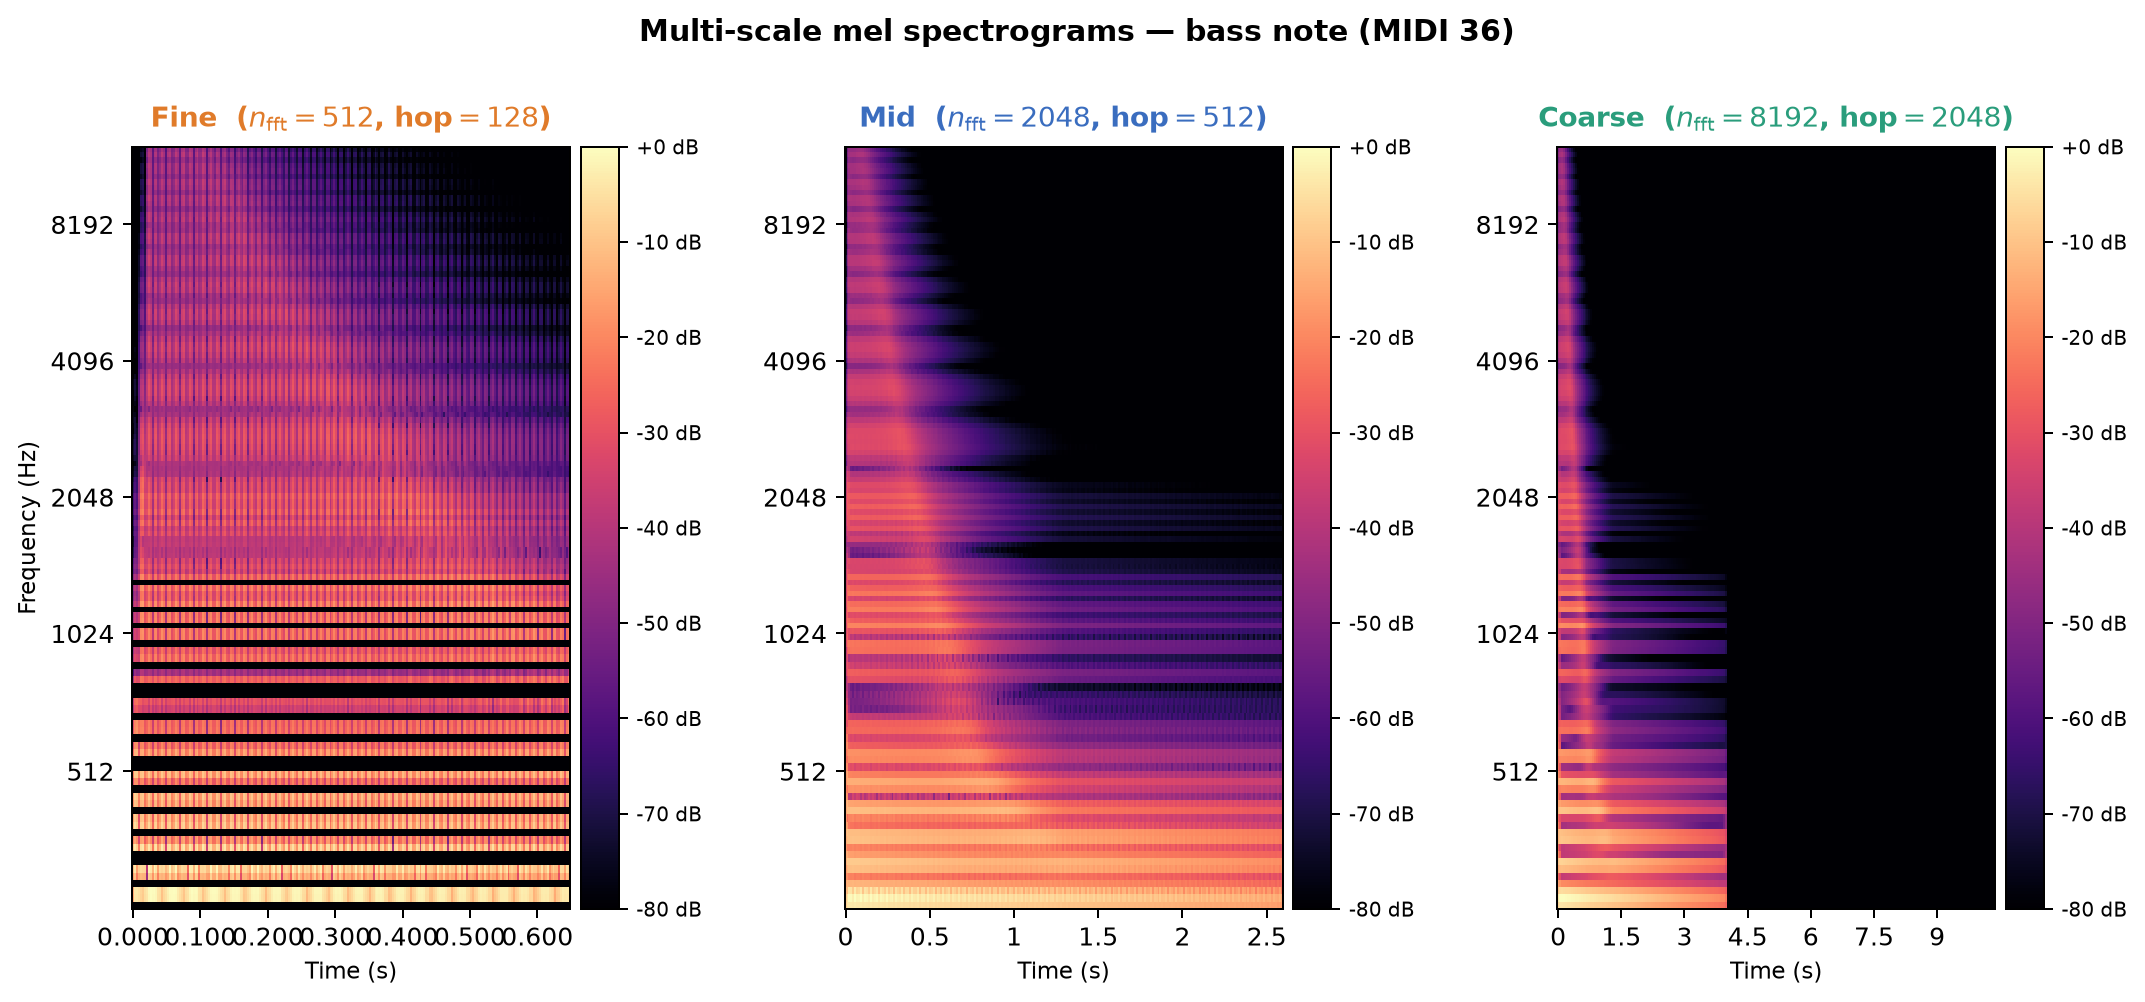
\includegraphics[width=\linewidth]{images/multiscale_mel_example.png}
\vspace{0.2cm}
\caption{Multi-scale mel spectrograms of a Vital bass note (MIDI 36) at fine ($n_{\text{fft}}=512$), mid ($n_{\text{fft}}=2{,}048$), and coarse ($n_{\text{fft}}=8{,}192$) resolutions. The fine scale resolves fast temporal events; the mid scale shows envelope shape and spectral balance; the coarse scale reveals the harmonic series structure. All three are padded or truncated to 224 time frames before stacking.}
\label{fig:multiscale_mel_example}
\end{figure}

\noindent The three spectrograms are stacked along the channel dimension to form a three-channel input tensor of shape $(3, 128, 224)$, as illustrated in Figure~\ref{fig:multiscale_stack}. This is directly compatible with the three-channel (RGB) first-layer weight initialization of ConvNeXt and ViT backbones.

\begin{figure}[H]
\centering
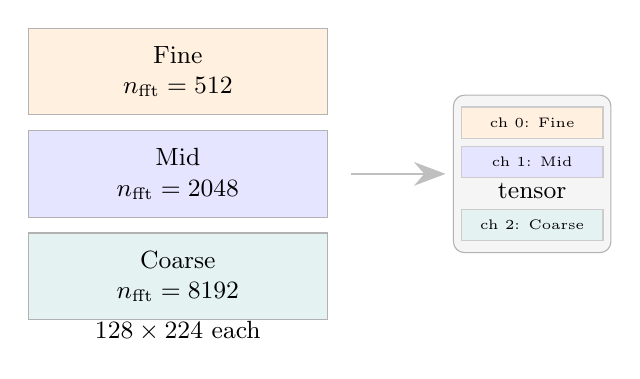
\begin{tikzpicture}[
  spec/.style={draw=gray!60, fill=blue!6, minimum width=3.8cm, minimum height=1.1cm,
               align=center, font=\small},
  label/.style={font=\small, align=center},
  arrow/.style={-{Stealth[length=4mm]}, thick, gray!50}
]

% Three spectrogram slabs
\node[spec, fill=orange!12] (fine)   at (0, 2.6) {Fine\\$n_{\text{fft}}=512$};
\node[spec, fill=blue!10]   (mid)    at (0, 1.3) {Mid\\$n_{\text{fft}}=2048$};
\node[spec, fill=teal!10]   (coarse) at (0, 0.0) {Coarse\\$n_{\text{fft}}=8192$};

\node[label] at (0, -0.7) {$128\times224$ each};

% Brace / arrow
\draw[arrow] (2.2, 1.3) -- (3.4, 1.3);

% Stacked tensor box
\draw[fill=gray!8, draw=gray!60, rounded corners=4pt]
  (3.5, 0.3) rectangle (5.5, 2.3);
\node[font=\small, align=center] at (4.5, 1.3)
  {$(3, 128, 224)$\\\small tensor};

% Channel labels inside
\draw[fill=orange!12, draw=gray!40] (3.6, 1.75) rectangle (5.4, 2.15);
\draw[fill=blue!10,   draw=gray!40] (3.6, 1.25) rectangle (5.4, 1.65);
\draw[fill=teal!10,   draw=gray!40] (3.6, 0.45) rectangle (5.4, 0.85);
\node[font=\tiny] at (4.5, 1.95) {ch 0: Fine};
\node[font=\tiny] at (4.5, 1.45) {ch 1: Mid};
\node[font=\tiny] at (4.5, 0.65) {ch 2: Coarse};

\end{tikzpicture}
\vspace{0.3cm}
\caption{Three mel spectrograms at fine, mid, and coarse resolutions stacked into a single three-channel input tensor of shape $(3, 128, 224)$.}
\label{fig:multiscale_stack}
\end{figure}

% ─────────────────────────────────────────────────────────
\subsubsection{Step 6: Dataset Splitting and Normalization}

\subsubsubsection{Stratified Split}

A purely random partition would not guarantee that each set reflects the full musical diversity of the dataset. By chance, all bass presets could land predominantly in the training set while the test set is dominated by pad or random presets, or an entire pitch register could be absent from validation entirely. Under such a split, the reported MAE would partly reflect a distribution mismatch rather than a genuine measure of model generalisation. The stratified split prevents this by treating the joint timbre-and-pitch-register label as a stratum and allocating samples from each stratum in the target 80\,/\,10\,/\,10 ratio independently, ensuring that every timbre category and every pitch register appears in proportional numbers across all three partitions. This guarantees that the evaluation sets are musically representative: the model is tested on the same joint distribution of sounds it was trained on, so MAE differences between configurations reflect differences in model quality rather than accidents of split composition.

Each sample is assigned a bucket key combining its timbre label and the octave of its MIDI note:

\begin{equation}
\text{bucket} = \left(\text{timbre},\; \left\lfloor \frac{\text{midi\_note}}{12} \right\rfloor\right)
\label{eq:bucket}
\end{equation}

\noindent Within each bucket, sample indices are deterministically shuffled using a seeded random number generator and then allocated in an 80\,/\,10\,/\,10 ratio to training, validation, and test sets in that order. A guard ensures that at least one sample from every non-empty bucket falls in the training partition, preventing pathologically small strata from being entirely consumed by the test allocation. Five independent splits are generated using seeds 42 through 46, producing five-fold cross-validation partitions for robust evaluation of the $\approx 42{,}520$-sample V1/V2 dataset. Reporting test MAE as mean $\pm$ standard deviation across the five folds controls for the variance introduced by any single arbitrary split.

\par \vspace{0.3cm}
In V3, sample-level splitting introduces a data leakage problem that does not exist in V1 or V2. Because each preset is rendered at three MIDI pitches, a sample-level split could assign two of a preset's renders to the training partition and the third to the test partition. As all three renders share the same parameter target $\mathbf{y}$, the model would have encountered those exact synthesis parameters during training, artificially deflating the reported test MAE. The V3 split therefore operates at the preset level: all renders of the same preset are treated as a single indivisible group, and entire groups are assigned to partitions rather than individual samples. The group key is computed as the MD5 hash of the 16 parameter values:

\begin{equation}
k(\theta) = \mathrm{MD5}\!\left(\theta_0,\, \theta_1,\, \ldots,\, \theta_{15}\right)
\label{eq:preset_key}
\end{equation}

\noindent This hash is deterministic and identical across all MIDI-note renders of the same preset without requiring a stored group identifier in the dataset. Figure~\ref{fig:preset_split} contrasts the two splitting strategies.

\begin{figure}[H]
\centering
\resizebox{\linewidth}{!}{%
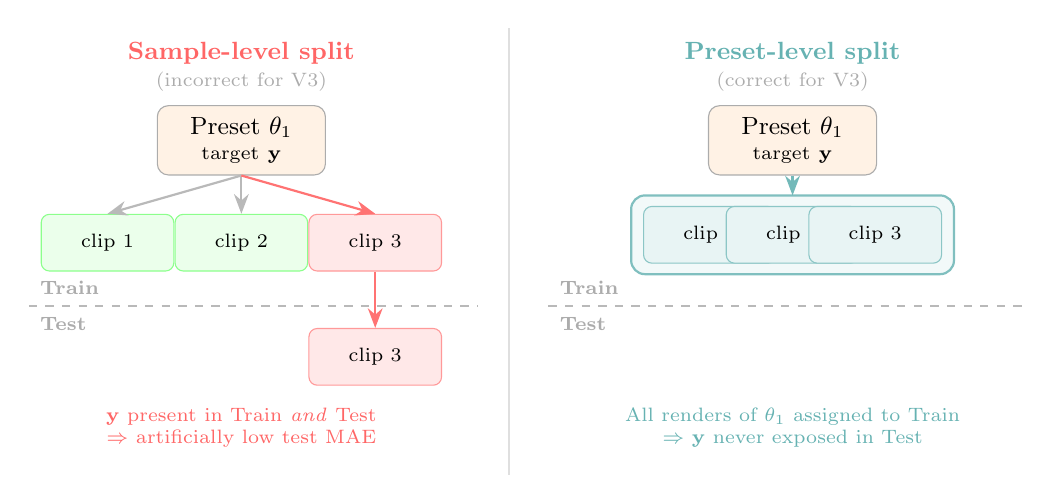
\begin{tikzpicture}[
  font=\small,
  cbox/.style={rectangle, rounded corners=3pt, draw=gray!55,
               minimum height=0.72cm, text width=1.45cm, align=center, font=\scriptsize},
  pbox/.style={rectangle, rounded corners=4pt, draw=gray!65, fill=orange!10,
               minimum height=0.88cm, text width=1.9cm, align=center},
  arr/.style={-{Stealth[length=2.5mm]}, thick, gray!55},
]

%% LEFT PANEL (incorrect)
\node[font=\small\bfseries, text=red!60]  at (-3.4, 5.4)  {Sample-level split};
\node[font=\scriptsize, text=gray!65]     at (-3.4, 5.05) {(incorrect for V3)};

\node[pbox] (PL) at (-3.4, 4.3)
  {Preset $\theta_1$\\[-2pt]\scriptsize target $\mathbf{y}$};

\node[cbox, fill=green!8, draw=green!45] (L1) at (-5.1, 3.0) {clip 1};
\node[cbox, fill=green!8, draw=green!45] (L2) at (-3.4, 3.0) {clip 2};
\node[cbox, fill=red!9,   draw=red!40]   (L3) at (-1.7, 3.0) {clip 3};

\draw[arr] (PL.south) -- (L1.north);
\draw[arr] (PL.south) -- (L2.north);
\draw[-{Stealth[length=2.5mm]}, thick, red!55] (PL.south) -- (L3.north);

\draw[dashed, gray!55, thick] (-6.1, 2.2) -- (-0.4, 2.2);
\node[font=\scriptsize\bfseries, text=gray!65, anchor=south west] at (-6.08, 2.22) {Train};
\node[font=\scriptsize\bfseries, text=gray!65, anchor=north west] at (-6.08, 2.18) {Test};

\node[cbox, fill=red!9, draw=red!40] (L3b) at (-1.7, 1.55) {clip 3};
\draw[-{Stealth[length=2.5mm]}, thick, red!55] (L3.south) -- (L3b.north);

\node[font=\scriptsize, text=red!60, align=center] at (-3.4, 0.65)
  {$\mathbf{y}$ present in Train \emph{and} Test\\
   $\Rightarrow$ artificially low test MAE};

%% SEPARATOR
\draw[gray!25, semithick] (0.0, 0.05) -- (0.0, 5.72);

%% RIGHT PANEL (correct)
\node[font=\small\bfseries, text=teal!60] at (3.6, 5.4)  {Preset-level split};
\node[font=\scriptsize, text=gray!65]     at (3.6, 5.05) {(correct for V3)};

\node[pbox] (PR) at (3.6, 4.3)
  {Preset $\theta_1$\\[-2pt]\scriptsize target $\mathbf{y}$};

\draw[rounded corners=5pt, draw=teal!50, fill=teal!5, thick]
  (1.55, 2.6) rectangle (5.65, 3.6);
\node[font=\scriptsize\bfseries, text=teal!60, anchor=north west]
  at (1.63, 3.53) {preset group};

\node[cbox, fill=teal!9, draw=teal!45] at (2.55, 3.1) {clip 1};
\node[cbox, fill=teal!9, draw=teal!45] at (3.60, 3.1) {clip 2};
\node[cbox, fill=teal!9, draw=teal!45] at (4.65, 3.1) {clip 3};

\draw[-{Stealth[length=2.5mm]}, thick, teal!55] (PR.south) -- (3.6, 3.6);

\draw[dashed, gray!55, thick] (0.5, 2.2) -- (6.6, 2.2);
\node[font=\scriptsize\bfseries, text=gray!65, anchor=south west] at (0.52, 2.22) {Train};
\node[font=\scriptsize\bfseries, text=gray!65, anchor=north west] at (0.52, 2.18) {Test};

\node[font=\scriptsize, text=teal!60, align=center] at (3.6, 0.65)
  {All renders of $\theta_1$ assigned to Train\\
   $\Rightarrow$ $\mathbf{y}$ never exposed in Test};

\end{tikzpicture}%
}
\vspace{0.3cm}
\caption{Sample-level versus preset-level splitting for the V3 multi-pitch dataset. \textit{Left:} a sample-level split can assign different MIDI-note renders of the same preset to different partitions; since all renders share the same parameter target~$\mathbf{y}$, the model has already seen those exact parameters during training, causing leakage and an artificially low test MAE. \textit{Right:} the preset-level split groups all renders of a preset by the MD5 hash of their shared parameter values and assigns the entire group to one partition, ensuring the test set contains only unseen presets.}
\label{fig:preset_split}
\end{figure}

\noindent Groups are stratified by timbre rather than timbre $\times$ octave, because multi-pitch rendering already places each group across multiple octaves --- stratifying by octave would scatter a single preset's renders across strata rather than keeping them together as one group. Groups within each timbre stratum are shuffled with a fixed seed and divided 80\,/\,10\,/\,10 by group count. A single split is used for V3 rather than five-fold cross-validation, because the computational cost of training two backbone families on $\approx 136{,}000$ samples for 40 epochs renders five independent training runs impractical within the available hardware budget, and because the larger dataset substantially reduces the split-variance that motivated cross-validation at the V1/V2 scale.

\subsubsubsection{Normalization}

Three normalization schemes are applied across all versions, each fitted exclusively on the training partition and applied identically to validation and test sets to prevent any leakage of held-out statistics into the training process.

\par \vspace{0.3cm}
\textit{Mel spectrograms} are Z-score normalized per mel bin using statistics computed from the training partition only. In V1, a single set of per-bin statistics $(\mu_m, \sigma_m)$ is accumulated online over all time frames of the training mid-scale spectrograms and applied as:

\begin{equation}
\hat{S}(t, m) = \frac{S(t, m) - \mu_{\text{train}}}{\sigma_{\text{train}}}
\label{eq:zscore}
\end{equation}

\noindent In V2 and V3, three independent sets of statistics are computed --- one per scale (fine, mid, coarse). Each analysis window produces spectrograms with substantially different absolute energy levels and frequency distributions: the coarse scale concentrates energy into narrow harmonic bins and has a much lower broadband noise floor than the fine scale, which spreads energy broadly across time. Using a single global scaler across all three scales would conflate these different magnitude ranges and degrade normalization quality for the outer scales. Statistics are saved as compressed \texttt{.npz} files per split per scale and loaded at evaluation time, ensuring identical normalization is applied to validation and test sets.

\par \vspace{0.3cm}
\textit{Synthesizer parameters} are normalized to $[0, 1]$ per parameter, but the normalization scale depends on the physical nature of each parameter. The twelve oscillator, filter, modulation, and reverb parameters are normalized linearly:

\begin{equation}
\hat{x}_k = \frac{x_k - x_k^{\min}}{x_k^{\max} - x_k^{\min}}, \quad k = 1, \ldots, 16
\label{eq:minmax}
\end{equation}

\noindent The four envelope time parameters (\texttt{env1\_attack}, \texttt{env1\_decay}, \texttt{env2\_attack}, \texttt{env2\_decay}) are instead normalized on a logarithmic scale, because envelope times span three orders of magnitude and exhibit perceptual logarithmic scaling --- a 10\,ms attack and a 100\,ms attack are as perceptually distinct as a 100\,ms and a 1{,}000\,ms attack. Equal spacing in log space therefore better represents equal perceptual step size than equal spacing in linear time:

\begin{equation}
\hat{x}_k = \frac{\log_{10}(x_k + \epsilon_t) - \log_{10}(x_k^{\min} + \epsilon_t)}%
                 {\log_{10}(x_k^{\max} + \epsilon_t) - \log_{10}(x_k^{\min} + \epsilon_t)},
\quad k \in \mathcal{K}_{\log}
\label{eq:lognorm}
\end{equation}

\noindent where $\mathcal{K}_{\log} = \{\texttt{env1\_attack},\, \texttt{env1\_decay},\, \texttt{env2\_attack},\, \texttt{env2\_decay}\}$ and $\epsilon_t = 10^{-4}$ prevents $\log_{10}(0)$ for near-zero time values. The filter cutoff, expressed in semitones, is normalized linearly since the semitone scale is already logarithmic with respect to frequency.

\par \vspace{0.3cm}
\textit{MIDI pitch} is normalized to $[0, 1]$ using the fixed global range $[12, 84]$:

\begin{equation}
p = \frac{\text{midi\_note} - 12}{84 - 12}
\label{eq:pitch_norm}
\end{equation}

\noindent This normalized scalar $p \in [0, 1]$ is then passed through a sinusoidal embedding to produce a rich 128-dimensional Fourier feature vector:

\begin{equation}
\boldsymbol{\phi}(p) = \left[\sin(\omega_0 p),\, \cos(\omega_0 p),\, \sin(\omega_1 p),\, \cos(\omega_1 p),\, \ldots,\, \sin(\omega_{63} p),\, \cos(\omega_{63} p)\right]
\label{eq:sinusoidal}
\end{equation}

\noindent where the frequencies $\omega_k = 2^k \cdot \pi$ are log-spaced from $\omega_0 = \pi$ to $\omega_{63} = 2^{63}\pi$. This avoids float32 overflow from naive power scaling and provides the model with a dense, multi-frequency representation of the pitch scalar. The final dataset sizes after filtering and splitting are summarized in Table~\ref{tab:dataset_sizes}.

\begin{table}[H]
\centering
\renewcommand{\arraystretch}{1.3}
\begin{tabular}{lcccccc}
\hline
\textbf{Version} & \textbf{Presets} & \textbf{Pitches / Preset} & \textbf{Total Samples} & \textbf{Train} & \textbf{Val} & \textbf{Test} \\
\hline
V1 / V2 & $\approx$42{,}250 & 1       & $\approx$42{,}250  & $\approx$33{,}800  & $\approx$4{,}225  & $\approx$4{,}225  \\
V3      & $\approx$42{,}250 & 3 or 4  & $\approx$168{,}000 & $\approx$134{,}400 & $\approx$16{,}800 & $\approx$16{,}800 \\
\hline
\end{tabular}
\vspace{0.3cm}
\caption{Dataset sizes across experimental versions. V3 ``pitches / preset'' is 3 if the V1/V2 random note coincides with one of the three fixed notes (that render is reused), or 4 otherwise; four is the typical outcome. Splits are performed at preset level in all versions to prevent leakage.}
\label{tab:dataset_sizes}
\end{table}

% ═══════════════════════════════════════════════════════════
\subsection{Iteration 1: Baseline Architecture and Pitch Conditioning}

\noindent
The first iteration establishes a controlled baseline by training and comparing three backbone architecture families — a custom residual CNN, an Audio Spectrogram Transformer, and a ConvNeXt — across three pitch conditioning strategies, using a single-scale mel spectrogram as input. The goal is to determine which combination achieves the lowest mean absolute error on the Vital parameter estimation task and to identify which directions are most promising for subsequent architectural refinement.

\subsubsection{Problem Investigation}

\noindent
Prior to this study, parameter estimation for the Vital wavetable synthesizer had not been addressed. Bruford et al.\ \cite{bruford2024ast} applied an AST to Massive, a modern wavetable synthesizer by Native Instruments, while InverSynth \cite{barkan2019inversynth} and Sound2Synth \cite{chen2022sound2synth} target FM and subtractive synthesizers respectively. Although Vital is a wavetable instrument, the 16-parameter subset studied here is deliberately structured to replicate a classic subtractive signal chain: two wavetable oscillators and one noise oscillator feed a low-pass filter whose cutoff is modulated by a dedicated filter envelope (Envelope 2) scaled by a modulation amount parameter; the resulting signal then passes through an amplitude envelope (Envelope 1) before a global reverb stage. Despite this subtractive signal-flow topology, the wavetable oscillators introduce a continuous, high-dimensional waveform space not present in conventional subtractive or FM instruments. It is therefore unknown whether the inductive biases of convolutional models, which capture local spectral patterns, outperform those of Transformer-based models, which model long-range dependencies across the full time-frequency plane, when the target synthesizer combines a structured analog signal chain with a wavetable oscillator stage.

\noindent \newline
A second open question concerns the role of explicit pitch conditioning. No prior work on synthesizer parameter estimation incorporates the MIDI pitch as a direct model input. Although the fundamental frequency of the rendered note is implicitly present in the mel spectrogram — manifesting as the position of the harmonic series along the frequency axis — it is unclear whether the model can reliably extract and exploit this information without guidance. Providing the normalised MIDI pitch as an explicit conditioning signal may yield more robust predictions across the pitch range, particularly for pitch-sensitive parameters such as oscillator transposition, where the correct prediction is directly related to the input pitch. It is additionally unclear whether a basic linear pitch projection is sufficient or whether a richer, multi-frequency sinusoidal encoding is needed to exploit pitch information effectively. This iteration therefore investigates the following questions:
\begin{itemize}
    \item Which backbone architecture — custom CNN, AST, or ConvNeXt — best captures wavetable timbral features from a single-scale mel spectrogram?
    \item Does explicit pitch conditioning reduce parameter estimation error, and does a sinusoidal Fourier embedding outperform a basic MLP projection?
\end{itemize}

\subsubsection{Solution Design}

\noindent
The solution design for V1 consists of six model configurations arising from the combination of two backbone families (AST-small and ConvNeXt-tiny; the custom CNN baseline was included as a lightweight reference) with three pitch conditioning strategies. All configurations share the same input format — a single mid-scale mel spectrogram of shape $128 \times 224$ — and the same output layer — a Sigmoid-activated linear projection to 16 normalised parameters.

\noindent \newline
The three backbone families differ in their inductive bias and pre-training. The \textbf{SynthParamNet} (baseline CNN) is a custom residual network with a hybrid pooling strategy: the frequency axis is collapsed by global average pooling, and the resulting time sequence is reduced by concatenating a max-pool and an average-pool, yielding a $2C$-dimensional embedding that handles variable-length time axes without requiring zero-padding. The \textbf{AST-small} is a pre-trained Vision Transformer (ViT-small/16) \cite{dosovitskiy2021vit, gong2021ast} adapted to mono spectrogram input by retaining the first-channel slice of the RGB stem; the CLS token serves as the global representation. The \textbf{ConvNeXt-tiny} is a pre-trained convolutional backbone \cite{liu2022convnext} with ImageNet-22k weights, adapted to mono input in the same way and pooled with the same hybrid strategy as the baseline CNN.

\noindent \newline
For each backbone, three pitch conditioning variants are evaluated: \textbf{no-pitch}, in which the mel embedding feeds directly to the regression head; \textbf{basic MLP}, in which the normalised MIDI scalar $p \in [0,1]$ passes through a two-layer MLP and its output is concatenated with the mel embedding; and \textbf{sinusoidal embedding}, in which $p$ is first mapped to a 128-dimensional Fourier feature vector $\boldsymbol{\phi}(p)$ (Equation~\ref{eq:sinusoidal}) before the same MLP, providing a richer multi-frequency representation of the pitch scalar. Figure~\ref{fig:v1_design} illustrates the overall V1 design.

\begin{figure}[H]
\centering
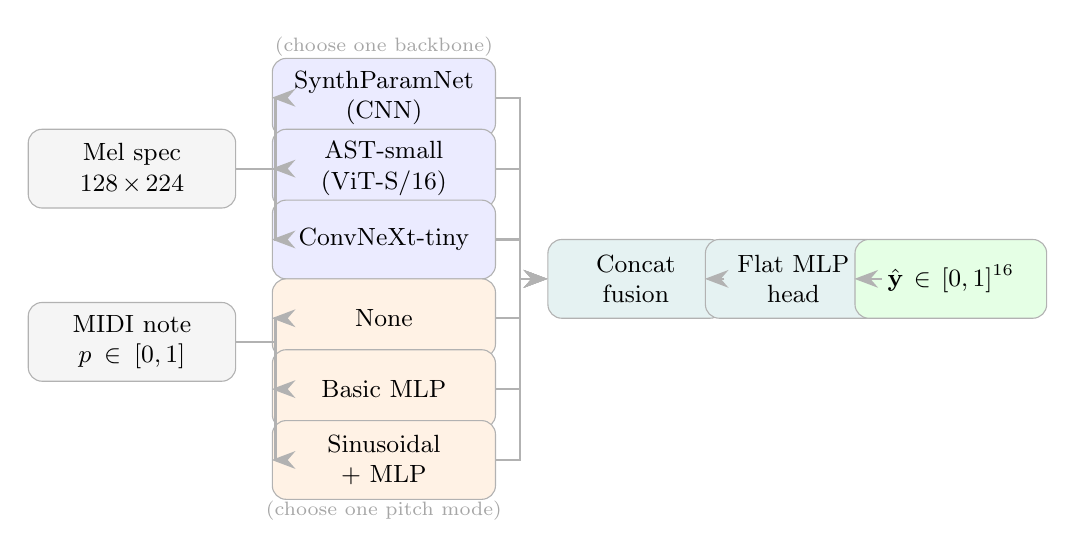
\begin{tikzpicture}[
  font=\small,
  node distance=0.55cm and 1.0cm,
  bb/.style={rectangle, rounded corners=5pt, draw=gray!60, fill=blue!8,
             minimum height=1.0cm, text width=2.6cm, align=center},
  pc/.style={rectangle, rounded corners=5pt, draw=gray!60, fill=orange!10,
             minimum height=1.0cm, text width=2.6cm, align=center},
  fuse/.style={rectangle, rounded corners=5pt, draw=gray!60, fill=teal!10,
               minimum height=1.0cm, text width=2.0cm, align=center},
  outbox/.style={rectangle, rounded corners=5pt, draw=gray!60, fill=green!10,
              minimum height=1.0cm, text width=2.2cm, align=center},
  inp/.style={rectangle, rounded corners=5pt, draw=gray!60, fill=gray!8,
              minimum height=1.0cm, text width=2.4cm, align=center},
  arrow/.style={-{Stealth[length=3mm]}, thick, gray!60}
]

% Input
\node[inp] (mel) at (0, 0) {Mel spec\\$128\!\times\!224$};
\node[inp] (pitch) at (0, -2.2) {MIDI note\\$p \in [0,1]$};

% Backbone options (stacked vertically)
\node[bb] (cnn)   at (3.2,  0.9) {SynthParamNet\\(CNN)};
\node[bb] (ast)   at (3.2,  0.0) {AST-small\\(ViT-S/16)};
\node[bb] (cnxt)  at (3.2, -0.9) {ConvNeXt-tiny};

% Pitch options (stacked)
\node[pc] (nopitch) at (3.2, -1.9) {None};
\node[pc] (mlp)     at (3.2, -2.8) {Basic MLP};
\node[pc] (sin)     at (3.2, -3.7) {Sinusoidal\\+ MLP};

% Fusion
\node[fuse] (fuse) at (6.4, -1.4) {Concat\\fusion};

% Head + Output
\node[fuse] (head) at (8.4, -1.4) {Flat MLP\\head};
\node[outbox]  (outp) at (10.4, -1.4) {$\hat{\mathbf{y}} \in [0,1]^{16}$};

% Arrows: mel → backbones
\draw[arrow] (mel.east) -- ++(0.5,0) |- (cnn.west);
\draw[arrow] (mel.east) -- ++(0.5,0) |- (ast.west);
\draw[arrow] (mel.east) -- ++(0.5,0) |- (cnxt.west);

% Arrows: pitch → pitch modules
\draw[arrow] (pitch.east) -- ++(0.5,0) |- (nopitch.west);
\draw[arrow] (pitch.east) -- ++(0.5,0) |- (mlp.west);
\draw[arrow] (pitch.east) -- ++(0.5,0) |- (sin.west);

% Arrows: backbones → fusion
\draw[arrow] (cnn.east)  -- ++(0.3,0) |- (fuse.west);
\draw[arrow] (ast.east)  -- ++(0.3,0) |- (fuse.west);
\draw[arrow] (cnxt.east) -- ++(0.3,0) |- (fuse.west);

% Arrows: pitch modules → fusion
\draw[arrow] (nopitch.east) -- ++(0.3,0) |- (fuse.west);
\draw[arrow] (mlp.east)     -- ++(0.3,0) |- (fuse.west);
\draw[arrow] (sin.east)     -- ++(0.3,0) |- (fuse.west);

% Head → Output
\draw[arrow] (fuse) -- (head);
\draw[arrow] (head) -- (outp);

% Brace labels
\node[font=\scriptsize, text=gray!70] at (3.2, 1.55) {(choose one backbone)};
\node[font=\scriptsize, text=gray!70] at (3.2, -4.35) {(choose one pitch mode)};

\end{tikzpicture}
\vspace{0.3cm}
\caption{V1 design space: three backbone options combined with three pitch conditioning strategies, converging on a shared concatenation-based fusion and flat regression head.}
\label{fig:v1_design}
\end{figure}

\noindent
Both AST and ConvNeXt are initialised from ImageNet-22k pre-trained weights, with their first-layer convolution adapted from three-channel (RGB) to one-channel (mono spectrogram) input by retaining only the first channel's weight slice. The sinusoidal pitch embedding $\boldsymbol{\phi}(p)$ uses log-spaced frequencies (Equation~\ref{eq:sinusoidal}) to avoid float32 overflow and to provide the model with a dense, multi-scale encoding of the pitch scalar.

\subsubsection{Design Validation}

\noindent
Before full-scale training, the following validation checks were performed to ensure the correctness of the V1 design:

\begin{itemize}
    \item \textbf{Architecture Compatibility:} Single-channel stem adaptation was verified for both AST and ConvNeXt by confirming that the adapted first layer produced activations of the correct spatial shape ($128 \times 224$ feature maps at the input resolution). For AST, the \texttt{dynamic\_img\_size=True} flag was confirmed to handle the non-square $128 \times 224$ input without positional embedding mismatch.

    \item \textbf{Sinusoidal Embedding Numerical Safety:} The log-spaced frequencies $\omega_k = 2^k \pi$ were verified to remain within float32 range at $k = 63$ ($\omega_{63} = 2^{63}\pi \approx 2.9 \times 10^{19}$); because these values enter only as arguments to $\sin$ and $\cos$, no overflow occurs in the embedding vector.

    \item \textbf{Baseline Calibration Against Prior Work:} The AST-small no-pitch configuration approximates the essential setup of Bruford et al.\ \cite{bruford2024ast} — a ViT encoder, single-scale mel spectrogram input, and no pitch conditioning — to provide a reference point against the primary baseline in the literature. The replication is intentionally partial: Bruford et al.\ use a Mean Squared Error (MSE) loss during training and scale their dataset to up to one million samples, both of which are beyond the scope of this study due to computational resource constraints. The AST-small no-pitch result therefore serves as a reference rather than a strict reproduction.

    \item \textbf{Data Split Integrity:} The five-fold stratified splits (Section~\ref{sec:methodology}) were verified to contain no preset identifier shared between any training and test partition, ensuring that evaluation MAE reflects generalisation to unseen presets rather than memorisation.
\end{itemize}

\noindent
These checks confirmed that the six V1 configurations were correctly implemented and that the AST-small no-pitch variant would serve as a valid reference against prior work.

\subsubsection{Solution Implementation}

\noindent
The following steps describe the technical implementation of the six V1 configurations.

\paragraph{1) Single-Scale Mel Spectrogram Extraction}
Each audio clip is converted to a mel spectrogram using the mid-scale configuration: FFT size $n_{\text{fft}}=2{,}048$, hop length $H=512$, 128 mel bins between 20 Hz and 12{,}000 Hz (Table~\ref{tab:mel_scales}). The resulting $128 \times T$ matrix is stored as a \texttt{.npy} file. At training time, each spectrogram is padded with the minimum value or truncated along the time axis to produce a fixed $128 \times 224$ tensor, which is then Z-score normalised using training-split statistics.

\paragraph{2) Backbone Adaptation to Mono Input}
For the \textbf{SynthParamNet CNN}, the encoder consists of a convolutional stem followed by $N$ residual stages, each doubling the channel count; the final feature map is reduced to a $2C$-dimensional embedding by frequency-axis average pooling followed by time-axis max-pool $\oplus$ average-pool concatenation. For \textbf{AST-small}, the first patch-embedding convolution — originally expecting three RGB channels — is adapted by retaining the weights of the first channel: $W_{\text{mono}} = W_{\text{RGB},0}$. The CLS token of the final transformer layer serves as the $d$-dimensional mel embedding. For \textbf{ConvNeXt-tiny}, the same single-channel weight slice is used at the stem, followed by the same hybrid pooling as the CNN: $\mathbf{z} = [\text{MaxPool}(\mathbf{F});\, \text{AvgPool}(\mathbf{F})] \in \mathbb{R}^{2C}$.

\paragraph{3) Pitch Conditioning Variants}
Given the normalised MIDI pitch $p = (\text{midi} - 12) / (84 - 12) \in [0,1]$, three conditioning branches are implemented.
In the \textbf{no-pitch} variant, no pitch information enters the model; the mel embedding $\mathbf{z}$ feeds directly to the head.
In the \textbf{basic MLP} variant, $p$ passes through a two-layer MLP (Linear $\to$ ReLU $\to$ Linear) producing a 64-dimensional pitch vector $\mathbf{e}_p$, which is concatenated with $\mathbf{z}$: $\mathbf{z}_{\text{fused}} = [\mathbf{z};\, \mathbf{e}_p]$.
In the \textbf{sinusoidal embedding} variant, $p$ is first encoded by $\boldsymbol{\phi}(p)$ (Equation~\ref{eq:sinusoidal}) before the same two-layer MLP, yielding a richer frequency-domain representation of pitch.

\paragraph{4) Flat Regression Head}
All six V1 configurations share the same three-layer regression head applied to the fused embedding:
\begin{equation}
    \hat{\mathbf{y}} = \sigma\!\left(W_3\, \text{ReLU}\!\left(W_2\, \text{ReLU}\!\left(W_1\, \mathbf{z}_{\text{fused}} + \mathbf{b}_1\right) + \mathbf{b}_2\right) + \mathbf{b}_3\right) \in [0,1]^{16}
    \label{eq:flat_head}
\end{equation}
where $W_1 \in \mathbb{R}^{256 \times d_{\text{fused}}}$, $W_2 \in \mathbb{R}^{128 \times 256}$, $W_3 \in \mathbb{R}^{16 \times 128}$, and $\sigma$ is the element-wise Sigmoid function. The Sigmoid output bounds all predictions to $[0, 1]$, matching the normalised parameter range.

\paragraph{5) Training Protocol}
All models are trained with the Adaptive Moment Estimation with Weight Decay (AdamW) optimiser (weight decay $10^{-4}$) for 100 epochs per fold. The batch size and base learning rate are architecture-dependent: the lightweight SynthParamNet CNN uses a larger batch size and higher learning rate, while the pre-trained ConvNeXt-tiny and AST-small backbones use smaller batch sizes and lower learning rates suited to fine-tuning large pre-trained models. For pre-trained backbones (AST, ConvNeXt), a differential learning rate is applied: the backbone parameters are updated at $0.1\times$ the head learning rate to preserve the ImageNet-22k representations during early fine-tuning. A cosine-annealing OneCycleLR scheduler with $\text{pct\_start}=0.3$ is used to warm up the learning rate over the first 30\% of training before annealing. AMP training is enabled on the NVIDIA RTX 4090 with gradient clipping at $\text{max\_norm}=1.0$. The training loss is the standard (unweighted) SmoothL1 loss with $\beta=0.02$.

\paragraph{6) Five-Fold Cross-Validation}
Five independent stratified splits are generated from the V1/V2 dataset of $\approx 42{,}250$ samples using the timbre $\times$ octave bucket key (Equation~\ref{eq:bucket}). Each split produces a training set of $\approx 33{,}800$ samples and evaluation and test sets of $\approx 4{,}225$ samples each. For each fold, training is performed on the training partition and the model checkpoint with the lowest validation MAE is retained. Test MAE is reported as mean $\pm$ standard deviation across the five splits.

\subsubsection{Solution Evaluation}

\noindent
Three consistent patterns emerge from the five-fold test results. First, ConvNeXt-tiny outperforms AST-small in every pitch conditioning condition, with the gap ranging from 0.0007 to 0.0017 MAE. This indicates that, at the scale of $\approx 42{,}520$ training samples, the local convolutional inductive bias of ConvNeXt extracts more discriminative timbral features from mel spectrograms than the global self-attention of AST. Second, pitch conditioning consistently reduces MAE for both backbones. The improvement is most pronounced for the \texttt{oscillator\_2\_transpose} parameter, whose prediction benefits directly from knowing the absolute MIDI pitch: in the no-pitch ConvNeXt configuration this parameter's MAE is 0.101, compared to 0.090 with sinusoidal conditioning. Third, the sinusoidal embedding provides a small but consistent further improvement over the basic MLP for both backbones, supporting the hypothesis that a multi-frequency Fourier encoding represents pitch more effectively than a single linear projection.

\noindent \newline
Across all configurations, the seven oscillator parameters (wave frame, level, unison voices, unison detune for both oscillators, and transpose) consistently show the highest per-parameter MAE, typically in the range $0.08$–$0.16$. Envelope times and filter parameters, by contrast, fall below $0.05$ in all configurations. This difficulty gradient reflects the fact that wavetable position and unison settings map non-linearly to the mel spectrogram, whereas envelope shape is directly visible in the amplitude trajectory of the spectrogram.

\noindent \newline
These findings establish two clear directions for V2. The single-scale mid-resolution spectrogram sacrifices either temporal resolution (for transient capture) or spectral resolution (for harmonic analysis) — suggesting that a multi-resolution input could provide complementary information that reduces the oscillator parameter error. Additionally, the concatenation-based pitch conditioning adds pitch as a side input but does not allow it to modulate the timbral features already extracted by the backbone, limiting its effectiveness. Iteration 2 therefore introduces a multi-scale three-channel input and replaces concatenation-based conditioning with Feature-wise Linear Modulation.


% ═══════════════════════════════════════════════════════════
\subsection{Iteration 2: Multi-Scale Input, FiLM Conditioning, and Grouped Prediction}

\noindent
The second iteration introduces four architectural enhancements motivated by the limitations identified in V1: a multi-scale three-channel mel spectrogram input, Feature-wise Linear Modulation (FiLM) for pitch conditioning, a grouped prediction head, and a weighted training loss. The V1 backbone comparison is retained with both AST-small and ConvNeXt-tiny, now both trained with the full V2 architecture.

\subsubsection{Problem Investigation}

\noindent
V1 established that the single mid-scale mel spectrogram is the primary input representation. However, a single FFT window size enforces a fixed trade-off between time and frequency resolution. The mid-scale configuration ($n_{\text{fft}}=2{,}048$, hop$=512$) provides balanced resolution but is insufficient for resolving the fine harmonic structure that underlies wavetable timbres: discriminating between wavetable positions and oscillator waveforms requires the backbone to observe how individual harmonics are shaped and spaced, information that is best captured at long analysis windows. Conversely, the broad spectral morphology and coarse harmonic series structure that characterise pitch and tonal quality are most clearly visible at even longer windows. The primary motivation for stacking three resolutions is therefore to enrich the timbral and harmonic cues available to the backbone: the coarse scale ($n_{\text{fft}}=8{,}192$) exposes the harmonic series structure relevant to oscillator and pitch-sensitive parameters, the mid scale provides a balanced reference, and the fine scale ($n_{\text{fft}}=512$) adds short-time resolution that contributes complementary cues for transient and envelope-related features. All of this complementary information is entirely discarded in V1.

\noindent \newline
The second limitation concerns pitch conditioning. In V1, the pitch embedding is concatenated with the mel embedding after the backbone has finished processing the spectrogram. This late fusion means that the backbone extracts features without any awareness of pitch, and the pitch information enters only at the final fusion stage. Feature-wise Linear Modulation \cite{perez2018film} offers a more expressive alternative: it allows pitch to apply a learned affine transformation to the mel embedding, effectively modulating the feature representation before it enters the regression head. This conditional modulation is more expressive than concatenation because it enables pitch to suppress or amplify specific feature dimensions rather than merely appending new information.

\noindent \newline
A third limitation emerges from the V1 per-parameter analysis. Oscillator parameters have MAE values $2$–$3\times$ higher than envelope and filter parameters. A single flat regression head shared across all 16 parameters allocates identical capacity to easy and hard parameters alike, which is suboptimal when the prediction difficulty is highly non-uniform. This motivates a grouped prediction architecture that assigns wider, more expressive sub-networks to the harder oscillator group. This iteration therefore investigates:
\begin{itemize}
    \item Does stacking fine, mid, and coarse mel spectrograms as a three-channel input provide complementary time-frequency information that reduces MAE compared to the single mid-scale input?
    \item Does Feature-wise Linear Modulation provide a more effective pitch conditioning mechanism than concatenation-based fusion?
\end{itemize}

\subsubsection{Solution Design}

\noindent
The V2 solution introduces four changes applied uniformly to both the ConvNeXt-tiny and AST-small backbones. The first change replaces the single-scale mel input with a three-channel stack of fine, mid, and coarse spectrograms (Section~\ref{sec:methodology}, Figure~\ref{fig:multiscale_stack}), producing a $(3, 128, 224)$ input tensor directly compatible with the pre-trained RGB backbone stems. The second change replaces concatenation-based pitch conditioning with FiLM, which derives scale and shift parameters $(\boldsymbol{\gamma}, \boldsymbol{\beta})$ from the pitch embedding and applies them to the backbone output embedding. The third change introduces a grouped prediction head that assigns four specialised sub-MLPs to semantically related parameter groups, with the oscillator group receiving a wider sub-network to handle its higher prediction difficulty. The fourth change introduces a group-weighted SmoothL1 training objective that further focuses learning on the oscillator parameters by doubling their loss contribution. Figure~\ref{fig:v2_design} shows the complete V2 architecture.

\begin{figure}[H]
\centering
\resizebox{\linewidth}{!}{%
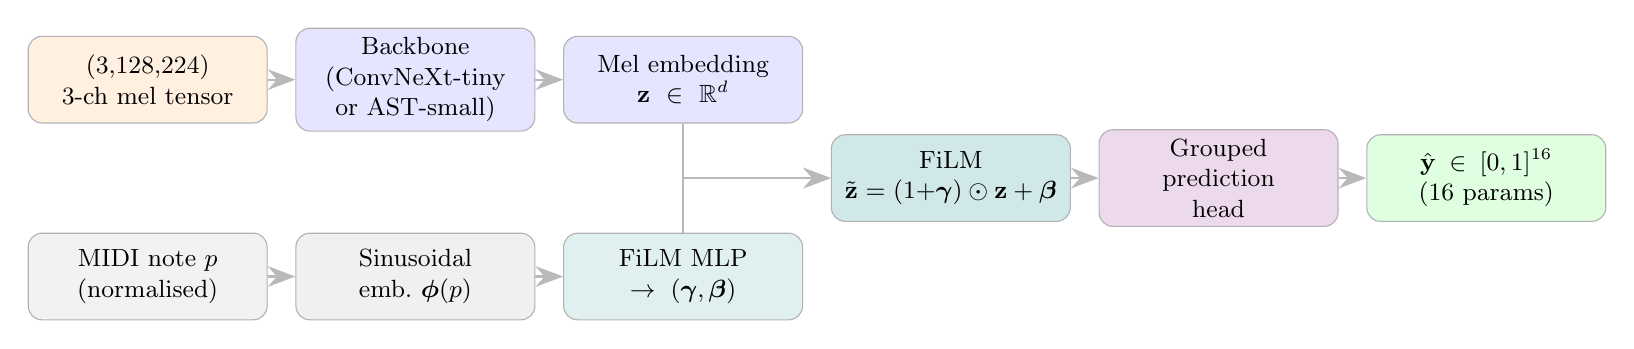
\begin{tikzpicture}[
  font=\small,
  node distance=0.55cm and 1.0cm,
  block/.style={rectangle, rounded corners=5pt, draw=gray!60, minimum height=1.1cm,
                align=center, text width=2.8cm},
  arrow/.style={-{Stealth[length=3.5mm]}, thick, gray!55}
]

% Input
\node[block, fill=orange!12] (mel) at (0,0)
  {$(3,\!128,\!224)$\\3-ch mel tensor};
\node[block, fill=gray!10] (pitch) at (0,-2.5)
  {MIDI note $p$\\(normalised)};

% Sinusoidal embedding
\node[block, fill=gray!12] (sinemb) at (3.4,-2.5)
  {Sinusoidal\\emb.\ $\boldsymbol{\phi}(p)$};

% Backbone
\node[block, fill=blue!10] (backbone) at (3.4,0)
  {Backbone\\(ConvNeXt-tiny\\or AST-small)};

% FiLM MLP
\node[block, fill=teal!12] (filmmlp) at (6.8,-2.5)
  {FiLM MLP\\$\rightarrow(\boldsymbol{\gamma},\boldsymbol{\beta})$};

% Embedding z
\node[block, fill=blue!10] (emb) at (6.8,0)
  {Mel embedding\\$\mathbf{z}\in\mathbb{R}^{d}$};

% FiLM box (centre)
\node[block, fill=teal!18] (film) at (10.2,-1.25)
  {FiLM\\$\tilde{\mathbf{z}}=(1{+}\boldsymbol{\gamma})\odot\mathbf{z}+\boldsymbol{\beta}$};

% Grouped head
\node[block, fill=violet!15] (head) at (13.6,-1.25)
  {Grouped\\prediction\\head};

% Output
\node[block, fill=green!12] (out) at (17.0,-1.25)
  {$\hat{\mathbf{y}}\in[0,1]^{16}$\\(16 params)};

% Arrows
\draw[arrow] (mel)     -- (backbone);
\draw[arrow] (backbone)-- (emb);
\draw[arrow] (emb)     |- (film.west);
\draw[arrow] (pitch)   -- (sinemb);
\draw[arrow] (sinemb)  -- (filmmlp);
\draw[arrow] (filmmlp) |- (film.west);
\draw[arrow] (film)    -- (head);
\draw[arrow] (head)    -- (out);

\end{tikzpicture}%
}
\vspace{0.3cm}
\caption{V2 (and V3) model architecture. The three-channel mel tensor is processed by the backbone into embedding $\mathbf{z}$; the FiLM conditioner derives $(\boldsymbol{\gamma},\boldsymbol{\beta})$ from the sinusoidal pitch embedding and applies an affine modulation; the grouped prediction head produces the 16 normalised parameter predictions.}
\label{fig:v2_design}
\end{figure}

\noindent
The FiLM conditioning and grouped head are formalized in Equations~\ref{eq:film_pred}--\ref{eq:weighted_loss} in the Solution Implementation below. The grouped head replaces the single flat MLP of V1 (Equation~\ref{eq:flat_head}) with four specialised sub-networks, each operating on the full modulated embedding $\tilde{\mathbf{z}}$ but predicting only its assigned parameter subset.

\subsubsection{Design Validation}

\noindent
The following validation checks were performed before full-scale V2 training:

\begin{itemize}
    \item \textbf{Three-Channel Weight Adaptation:} The adapted first-layer weights for the three-channel input were verified to preserve activation magnitudes. Averaging the three RGB weight slices and dividing by three ensures that a spectrogram tensor with values in the same range as an ImageNet image produces activations of the same expected magnitude as the original RGB stem, preventing the need for re-scaling the learning rate.

    \item \textbf{FiLM Identity Initialisation:} The FiLM MLP was initialised so that its output weights are zero, producing $\boldsymbol{\gamma}=\mathbf{0}$ and $\boldsymbol{\beta}=\mathbf{0}$ at epoch zero. This ensures that $\tilde{\mathbf{z}} = \mathbf{z}$ at initialisation, meaning V2 training begins from a state equivalent to the V1 no-pitch model, avoiding early-training instability caused by randomly-scaled feature modulations.

    \item \textbf{Grouped Head Output Consistency:} The four sub-MLP outputs were verified to be concatenated in the correct parameter order (indices 0–6, 7–10, 11–12, 13–15) to produce a 16-dimensional prediction vector, and the final Sigmoid activation was confirmed to bound all outputs to $[0,1]$.

    \item \textbf{Weighted Loss Gradient Balance:} Training loss logging confirmed that the doubled weight applied to the oscillator group ($w_{\text{osc}}=2$) produces proportionally larger gradients for indices 0–6, without causing gradient magnitude instability for the remaining parameter groups whose weights remain at 1.
\end{itemize}

\subsubsection{Solution Implementation}

\paragraph{1) Three-Channel Input Construction}
The three mel spectrograms extracted at fine, mid, and coarse resolutions (Table~\ref{tab:mel_scales}) are each padded or truncated to $128 \times 224$ and Z-score normalised independently using training-split statistics. The three normalised matrices are then stacked along the channel dimension to form the $(3, 128, 224)$ input tensor supplied to the backbone.

\paragraph{2) Backbone Adaptation to Three-Channel Input}
Both ConvNeXt-tiny and AST-small are adapted from RGB three-channel to audio three-channel input by averaging the pre-trained RGB stem weights across the colour dimension and scaling:
\begin{equation}
    W_{\text{audio}} = \frac{1}{3}\sum_{c=1}^{3} W_{\text{RGB},c}
    \label{eq:weight_adapt}
\end{equation}
This initialisation ensures that, in expectation, a spectrogram tensor at typical normalised magnitude produces the same activation statistics as an RGB image, allowing the pre-trained deeper layers to function correctly from the first forward pass.

\paragraph{3) FiLM Pitch Conditioning}
Given the sinusoidal pitch embedding $\boldsymbol{\phi}(p) \in \mathbb{R}^{128}$, a two-layer MLP predicts the FiLM scale and shift parameters:
\begin{equation}
    (\boldsymbol{\gamma},\, \boldsymbol{\beta}) = \text{MLP}_{\text{FiLM}}\!\left(\boldsymbol{\phi}(p)\right), \qquad \boldsymbol{\gamma},\, \boldsymbol{\beta} \in \mathbb{R}^{d}
    \label{eq:film_pred}
\end{equation}
The modulated embedding is then computed as:
\begin{equation}
    \tilde{\mathbf{z}} = (1 + \boldsymbol{\gamma}) \odot \mathbf{z} + \boldsymbol{\beta}
    \label{eq:film_apply}
\end{equation}
where $\odot$ denotes element-wise multiplication and $d$ is the backbone output dimension. The multiplicative term $(1 + \boldsymbol{\gamma})$ allows the conditioning to scale individual feature dimensions up or down based on pitch, while the additive term $\boldsymbol{\beta}$ shifts them; together they provide a more expressive transformation than the additive-only concatenation of V1.

\paragraph{4) Grouped Prediction Head}
The modulated embedding $\tilde{\mathbf{z}}$ is fed to four specialised sub-MLPs, one per parameter group. Table~\ref{tab:grouped_head} details the group composition and hidden widths.

\begin{table}[H]
\centering
\renewcommand{\arraystretch}{1.3}
\begin{tabular}{llcc}
\hline
\textbf{Group} & \textbf{Parameters (indices)} & \textbf{Count} & \textbf{Width} \\
\hline
Oscillator & \texttt{osc1\_wave\_frame}, \texttt{osc1\_level}, \texttt{osc1\_unison\_voices}, & 7 & $2h$ \\
           & \texttt{osc1\_unison\_detune}, \texttt{osc2\_wave\_frame}, \texttt{osc2\_level}, & & \\
           & \texttt{osc2\_transpose} \hspace{0.2em}(indices 0–6) & & \\
Envelope   & \texttt{env1\_attack}, \texttt{env1\_decay}, \texttt{env2\_attack},   & 4 & $h/2$ \\
           & \texttt{env2\_decay} \hspace{0.2em}(indices 7–10)                     & & \\
Filter     & \texttt{filter1\_cutoff}, \texttt{filter1\_resonance} \hspace{0.2em}(indices 11–12) & 2 & $h/2$ \\
Misc       & \texttt{sample\_level}, \texttt{mod1\_amount}, \texttt{reverb\_mix} \hspace{0.2em}(indices 13–15) & 3 & $h/2$ \\
\hline
\end{tabular}
\vspace{0.3cm}
\caption{Grouped prediction head structure. $h$ denotes the base hidden dimension; the oscillator group receives a wider sub-network ($2h$) to accommodate its higher prediction complexity.}
\label{tab:grouped_head}
\end{table}

\noindent Each sub-MLP produces its group's predictions via:
\begin{equation}
    \hat{\mathbf{y}}_g = \sigma\!\left(\text{MLP}_g(\tilde{\mathbf{z}})\right), \quad g \in \{1, 2, 3, 4\}
    \label{eq:grouped_head}
\end{equation}
The final prediction is the concatenation $\hat{\mathbf{y}} = [\hat{\mathbf{y}}_1;\, \hat{\mathbf{y}}_2;\, \hat{\mathbf{y}}_3;\, \hat{\mathbf{y}}_4] \in [0,1]^{16}$.

\paragraph{5) Weighted SmoothL1 Training Objective}
The training loss is a group-weighted SmoothL1 loss with $\beta=0.02$:
\begin{equation}
    \mathcal{L} = \sum_{g=1}^{4} w_g \cdot \text{SmoothL1}_{\beta}\!\left(\hat{\mathbf{y}}_g,\, \mathbf{y}_g\right), \qquad w_{\text{osc}} = 2,\quad w_g = 1 \text{ otherwise}
    \label{eq:weighted_loss}
\end{equation}
The oscillator group receives double weight because its parameters are perceptually dominant in determining the timbral character of a synthesizer sound \cite{roads1996computer}, and because V1 results confirm they are the hardest to predict. The SmoothL1 formulation, quadratic near zero and linear in the tail, provides robustness against occasional large prediction errors on high-variance parameters.

\paragraph{6) Training Protocol}
All V2 models are trained for 40 epochs per fold. The batch size is architecture-dependent — 128 or 256 depending on the model family — reflecting the different memory footprints of the SynthParamNet CNN, ConvNeXt-tiny, and AST-small. All other settings are inherited from V1: AdamW ($\text{wd}=10^{-4}$), differential learning rate ($0.1\times$ for backbone), OneCycleLR ($\text{pct\_start}=0.3$), AMP, and gradient clipping ($\text{max\_norm}=1.0$).

\paragraph{7) Ablation Design}
To isolate the contribution of FiLM pitch conditioning, each backbone is trained in two variants: the full V2 model (multi-scale input + FiLM + grouped head + weighted loss) and a no-pitch variant in which the FiLM branch is removed entirely and no pitch information enters the model, while all other components remain identical. This controlled comparison attributes any MAE difference exclusively to the presence of pitch conditioning.

\subsubsection{Solution Evaluation}

\noindent
The combined V2 enhancements produce a substantial reduction in MAE. The best V2 model, ConvNeXt-tiny-v2 with FiLM conditioning ($0.0665 \pm 0.0002$), improves over the V1 best ($0.0758 \pm 0.0005$) by approximately 12\%, confirming that the three-channel multi-scale input captures complementary time-frequency information that a single-scale representation cannot provide. ConvNeXt-tiny continues to outperform AST-small, now by a margin of 0.0048 MAE under FiLM conditioning.

\noindent \newline
FiLM conditioning provides a small but consistent improvement over the no-pitch variant for both backbones: $-0.0016$ MAE for ConvNeXt ($2.4\%$ reduction) and $-0.0014$ for AST ($1.9\%$ reduction). This improvement is statistically consistent across all five splits in both cases, confirming that the pitch information is genuinely useful. Nevertheless, the magnitude of the FiLM benefit is modest relative to the V1-to-V2 improvement, suggesting that the pitch conditioning pathway is not being fully exploited. Inspection of per-parameter results reveals that \texttt{osc2\_transpose} — the parameter most directly related to pitch — benefits from FiLM conditioning (its MAE drops from 0.078 to 0.076 in ConvNeXt), but the gain is smaller than expected for a parameter whose ground truth should be directly predictable from the MIDI note.

\noindent \newline
Beyond the limited FiLM benefit, both V2 models exhibit clear signs of overfitting: training MAE continues to decrease well below validation MAE, which plateaus around $0.055$–$0.060$ by epoch 30. This train-to-validation gap indicates that the $\approx 42{,}250$-sample dataset is insufficient to fully regularise models of this capacity. This combination of limited FiLM effectiveness and overfitting raises a critical question for Iteration 3: \textit{Is FiLM conditioning inherently insufficient for this task, or does its effectiveness depend on training data that presents the same preset parameter vector at multiple pitch positions — forcing the model to leverage pitch to resolve spectral ambiguity rather than relying solely on absolute spectral position?} To address both weaknesses simultaneously, Iteration 3 re-renders the existing $\approx 42{,}250$ presets at up to three fixed MIDI pitches each, rather than generating new presets. This approach expands the dataset to approximately $168{,}000$ samples after silence filtering while ensuring that the FiLM conditioning pathway receives meaningful cross-pitch variation: the same parameter target $\mathbf{y}$ now appears paired with multiple spectrally distinct inputs, directly testing whether pitch-aware training activates the FiLM pathway.


% ═══════════════════════════════════════════════════════════
\subsection{Iteration 3: Multi-Pitch Dataset Expansion and SpecAugment Regularisation}

\noindent
The third iteration addresses the two main weaknesses identified in V2 — limited FiLM conditioning effectiveness and mild overfitting — through changes to the training data regime rather than to the model architecture. The V2 architecture (Figure~\ref{fig:v2_design}) is retained without modification; the intervention is to re-render each preset at three distinct MIDI pitches per timbre and to introduce SpecAugment regularisation during training.

\subsubsection{Problem Investigation}

\noindent
In V1 and V2, every preset in the dataset is rendered at exactly one MIDI pitch, sampled uniformly from the timbre's valid range. This means that the model never observes the same parameter vector $\mathbf{y}$ at different spectral positions: each training sample is a unique (spectrogram, parameters) pair. A model in this setting can achieve low training loss by learning to associate specific absolute spectral patterns with parameter values, effectively using the pitch-dependent spectral position of harmonics as an implicit shortcut. Under this regime, the FiLM conditioning pathway receives no training pressure to actually modulate features based on pitch, because pitch-independent spectral matching is already sufficient to minimise the loss.

\noindent \newline
The training logs from V2 provide additional evidence of a generalisation problem: by epoch 30, both the ConvNeXt-tiny and AST-small models achieve training MAE values below $0.020$, while validation MAE plateaus around $0.055$–$0.060$. This train-to-validation gap indicates that the models have partially memorised spectral patterns specific to individual presets rather than learning a generalised mapping from timbre features to synthesis parameters. With only $\approx 42{,}250$ training samples shared across two backbones with 28M and 23M parameters respectively, regularisation through data diversity is a natural remedy.

\noindent \newline
\textit{Will rendering each preset at three distinct MIDI pitches — so that the model observes the same parameter vector $\mathbf{y}$ at three different spectral positions — activate the FiLM conditioning pathway and, combined with SpecAugment regularisation, reduce the train-to-validation gap?}

\subsubsection{Solution Design}

\noindent
The V3 solution addresses both weaknesses through a redesigned data generation regime. Each of the $\approx 42{,}250$ presets from the V1/V2 dataset is re-rendered at up to three fixed MIDI pitches per timbre, selected to cover the low, mid, and high registers of each timbre's valid range. The rendering pipeline uses a hash-based checkpoint system keyed on the (sorted preset parameters, MIDI note) pair: if the existing V1/V2 random note coincides with one of the three fixed notes, that render is already present and is skipped, and only the remaining two fixed notes are rendered; otherwise all three are rendered. Each preset therefore gains two or three new renderings in addition to its original V1/V2 render, giving three or four clips per preset in total — with four being typical since the random V1/V2 note rarely matches the fixed schedule. New renders are appended directly to the existing dataset file in append mode. After silence filtering, this expands the dataset from $\approx 42{,}250$ to $\approx 168{,}000$ samples. Crucially, each parameter vector $\mathbf{y}$ now appears paired with multiple spectrally distinct audio clips, providing the FiLM conditioning pathway with genuine cross-pitch training signal: it must learn to produce pitch-specific feature modulations that allow the same backbone embedding to be corrected for pitch-dependent spectral shift.

\noindent \newline
SpecAugment \cite{park2019specaugment} is introduced as an online training-time regulariser. Two time masks and two frequency masks are applied independently to each training sample per forward pass, preventing the model from over-relying on narrow spectral or temporal features and further increasing the effective diversity of the training distribution. Figure~\ref{fig:v3_design} illustrates the V3 data generation and augmentation pipeline.

\begin{figure}[H]
\centering
\resizebox{\linewidth}{!}{%
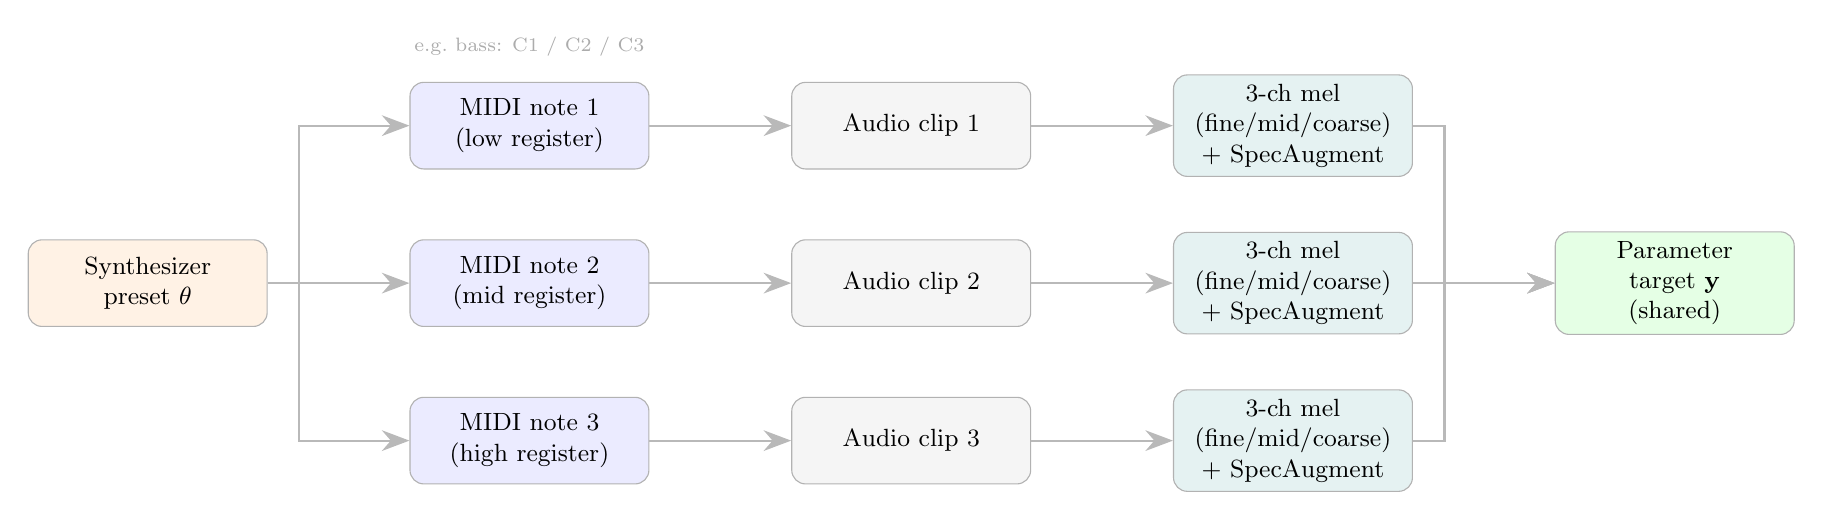
\begin{tikzpicture}[
  font=\small,
  node distance=0.6cm and 1.4cm,
  box/.style={rectangle, rounded corners=5pt, draw=gray!60, align=center,
              minimum height=1.1cm, text width=2.8cm},
  label/.style={font=\scriptsize, text=gray!65, align=center},
  arrow/.style={-{Stealth[length=3.5mm]}, thick, gray!55}
]

% Preset box
\node[box, fill=orange!10] (preset) {Synthesizer\\preset $\theta$};

% Three MIDI note boxes
\node[box, fill=blue!8,  right=1.8cm of preset, yshift= 2.0cm] (n1) {MIDI note 1\\(low register)};
\node[box, fill=blue!8,  right=1.8cm of preset, yshift= 0.0cm] (n2) {MIDI note 2\\(mid register)};
\node[box, fill=blue!8,  right=1.8cm of preset, yshift=-2.0cm] (n3) {MIDI note 3\\(high register)};

% Audio render boxes
\node[box, fill=gray!8, right=1.8cm of n1] (a1) {Audio clip 1};
\node[box, fill=gray!8, right=1.8cm of n2] (a2) {Audio clip 2};
\node[box, fill=gray!8, right=1.8cm of n3] (a3) {Audio clip 3};

% Three-channel mel boxes
\node[box, fill=teal!10, right=1.8cm of a1] (s1) {3-ch mel\\(fine/mid/coarse)\\+ SpecAugment};
\node[box, fill=teal!10, right=1.8cm of a2] (s2) {3-ch mel\\(fine/mid/coarse)\\+ SpecAugment};
\node[box, fill=teal!10, right=1.8cm of a3] (s3) {3-ch mel\\(fine/mid/coarse)\\+ SpecAugment};

% Label box (shared parameter target)
\node[box, fill=green!10, right=1.8cm of s2] (label) {Parameter\\target $\mathbf{y}$\\(shared)};

% Arrows: preset → MIDI notes
\draw[arrow] (preset.east) -- ++(0.4,0) |- (n1.west);
\draw[arrow] (preset.east) -- ++(0.4,0) |- (n2.west);
\draw[arrow] (preset.east) -- ++(0.4,0) |- (n3.west);

% Arrows: MIDI notes → audio
\draw[arrow] (n1) -- (a1);
\draw[arrow] (n2) -- (a2);
\draw[arrow] (n3) -- (a3);

% Arrows: audio → mel tensors
\draw[arrow] (a1) -- (s1);
\draw[arrow] (a2) -- (s2);
\draw[arrow] (a3) -- (s3);

% Arrows: mels → shared label
\draw[arrow] (s1.east) -- ++(0.4,0) |- (label.west);
\draw[arrow] (s2.east) -- (label.west);
\draw[arrow] (s3.east) -- ++(0.4,0) |- (label.west);

% Timbre note annotation
\node[label, above=0.2cm of n1] {e.g.\ bass: C1 / C2 / C3};

\end{tikzpicture}%
}
\vspace{0.3cm}
\caption{V3 data pipeline. Each preset is rendered at three fixed MIDI pitches, producing three spectrally different audio clips that share the same parameter target $\mathbf{y}$. Each clip is converted to a three-channel mel tensor (fine/mid/coarse); SpecAugment masks are applied online during training only.}
\label{fig:v3_design}
\end{figure}

\noindent
Because each preset now contributes multiple training samples (the original V1/V2 rendering plus up to three new fixed-note renders), the dataset split must be performed at the preset level to prevent leakage: all renderings of a given preset must be assigned to the same partition. This is a stricter requirement than the V1/V2 splits and is enforced through a preset-level grouping step before stratification.

\subsubsection{Design Validation}

\begin{itemize}
    \item \textbf{Preset-Level Split Integrity:} The splitting procedure was verified to assign all three pitch renderings of every preset to the same partition (training, validation, or test). A post-split check confirmed zero preset-ID overlap between the training and validation sets, ensuring that the validation MAE reflects generalisation to unseen presets rather than to unseen pitch renderings of known presets.

    \item \textbf{SpecAugment Parameter Selection:} Time mask width was capped at 30 frames ($\approx 3.5$ seconds at mid-scale hop) and frequency mask width at 15 mel bins (out of 128). These limits were selected to ensure that each masked spectrogram retains sufficient spectral content to identify the dominant timbre class, while providing enough stochastic variation to prevent feature co-adaptation.

    \item \textbf{MIDI Note Register Coverage:} The fixed MIDI note schedule per timbre (Table~\ref{tab:v3_midi}) was verified to span the low, mid, and high registers of each timbre's valid range, ensuring that for every timbre class the model encounters pitch variation across at least two octaves during training.

    \item \textbf{Shared Evaluation Protocol:} A fixed set of 100 held-out samples (\texttt{shared\_eval\_set.json}) was constructed from the V1/V2 test set, ensuring that both V2 and V3 models are evaluated on identical audio clips and preset parameter targets. This shared evaluation set enables a direct comparison of MSS values — which require Vital re-rendering — between versions without any confounding differences in evaluation samples.
\end{itemize}

\subsubsection{Solution Implementation}

\paragraph{1) Multi-Pitch Audio Rendering}
Each of the $\approx 42{,}250$ presets from the original dataset is re-rendered at up to three fixed MIDI pitches per timbre, following the schedule in Table~\ref{tab:v3_midi}. New renders are appended to the existing \texttt{combined\_dataset.jsonl} in append mode; a hash keyed on the (sorted preset parameters, MIDI note) pair detects any (preset, note) combination already present from V1/V2 and skips it. If the V1/V2 random note coincides with one of the three fixed notes, only the remaining two are rendered and the preset ends up with three clips; otherwise all three are rendered and the preset ends up with four clips. Four is the typical outcome since the random V1/V2 note rarely matches the fixed schedule. After silence filtering, the expanded dataset contains approximately $168{,}000$ samples — the original $\approx 42{,}250$ V1/V2 entries plus two or three new renders per preset.

\begin{table}[H]
\centering
\renewcommand{\arraystretch}{1.3}
\begin{tabular}{lcc}
\hline
\textbf{Timbre} & \textbf{MIDI notes} & \textbf{Pitch names} \\
\hline
bass   & 24, 36, 48 & C1, C2, C3 \\
lead   & 48, 60, 72 & C3, C4, C5 \\
pad    & 36, 54, 72 & C2, F$\sharp$3, C5 \\
percs  & 36, 60, 78 & C2, C4, F$\sharp$5 \\
random & 24, 48, 72 & C1, C3, C5 \\
\hline
\end{tabular}
\vspace{0.3cm}
\caption{Fixed MIDI pitches per timbre used in V3. For each preset, up to three new renders are produced at these notes; if the existing V1/V2 random note coincides with one fixed note, that render is reused and only the remaining two are rendered, leaving the preset with three or four clips in total.}
\label{tab:v3_midi}
\end{table}

\paragraph{2) SpecAugment Online Augmentation}
During training, each input tensor $(3, 128, 224)$ is augmented with two independent time masks (each with width drawn from $\mathcal{U}[0, 30]$ frames) and two independent frequency masks (each with width drawn from $\mathcal{U}[0, 15]$ mel bins). The same mask pattern is applied identically to all three channel slices of the tensor, preserving the inter-channel consistency of the fine, mid, and coarse spectrograms. Masked values are replaced with the global minimum of the normalised spectrogram. SpecAugment is disabled at validation and test time.

\paragraph{3) Preset-Level Dataset Split}
The $\approx 42{,}250$ unique presets are stratified by timbre and split 80/10/10 at the preset level, as described in Step~6 above. All renders of each preset follow their preset's partition assignment, producing $\approx 134{,}400$ training samples and $\approx 16{,}800$ validation and test samples respectively. A single split is used for V3 (rather than five-fold cross-validation) due to the computational cost of training two models on $\approx 134{,}400$ samples for 40 epochs.

\paragraph{4) Training Configuration}
The model architecture is identical to V2 (ConvNeXt-tiny and AST-small backbones, FiLM conditioning, grouped prediction head, weighted SmoothL1 loss). Training hyperparameters are also unchanged: AdamW ($\text{wd}=10^{-4}$), differential learning rate, OneCycleLR ($\text{pct\_start}=0.3$), 40 epochs, architecture-dependent batch size (128 or 256), AMP. SpecAugment augmentation is active during the forward passes on the training partition only.

\paragraph{5) MSS Evaluation Protocol}
Both V2 and V3 models are evaluated on the shared 100-sample held-out set using the Multi-Scale Spectral (MSS) loss as a perceptual complement to parameter MAE. For each sample, the predicted parameter vector $\hat{\mathbf{y}}$ is passed to Vital via Pedalboard to generate a re-rendered audio clip; the MSS loss is then computed as the mean absolute difference between the log-magnitude spectrograms of the original and re-rendered clips across four FFT scales ($n_{\text{fft}} \in \{128, 512, 2{,}048, 8{,}192\}$). A lower MSS value indicates a closer spectral match between original and predicted audio.

\paragraph{6) Ablation: FiLM vs No-Pitch Under V3}
The same FiLM-conditioned vs no-pitch comparison used in V2 is repeated under the V3 training regime, producing four models in total: ConvNeXt-tiny and AST-small, each in FiLM and no-pitch variants, all trained on the expanded multi-pitch dataset with SpecAugment. The change in the MAE gap between FiLM and no-pitch variants from V2 to V3 is the primary test of the multi-pitch training hypothesis.

\subsubsection{Solution Evaluation}

\noindent
Multi-pitch rendering and SpecAugment together produce the largest iteration-over-iteration improvement in the study. The best V3 model, AST-small-v2 with FiLM, achieves a MAE of $0.0525$ on the shared evaluation set, compared to $0.0713$ for the corresponding V2 model — a $26\%$ reduction. Both V3 models surpass all V2 models by a substantial margin, confirming that dataset scale and pitch diversity are the primary bottleneck that was limiting V2 performance.

\noindent \newline
The primary design hypothesis of V3 is confirmed by the evolution of the FiLM conditioning gap. In V2, FiLM conditioning already provides a small but consistent benefit on the five-fold test sets (ConvNeXt: FiLM $0.0665$ vs no-pitch $0.0681$; AST: FiLM $0.0713$ vs no-pitch $0.0727$), a gain of $0.0016$ and $0.0014$ respectively. In V3, this benefit is amplified for both backbones: $-0.0020$ MAE for ConvNeXt ($3.6\%$ improvement) and $-0.0035$ for AST ($6.3\%$ improvement). The larger FiLM gap in V3 confirms that multi-pitch training data enhances the effectiveness of pitch conditioning: when the model is forced to observe the same parameter vector at multiple spectral positions, the FiLM pathway receives stronger training signal and learns more expressive pitch-dependent modulations. The modest but non-zero V2 benefit suggests the pathway is already partially active on single-pitch data; V3's cross-pitch diversity amplifies it.

\noindent \newline
A second notable finding is the reversal of the ConvNeXt vs AST ranking. In V1 and V2, ConvNeXt-tiny consistently outperformed AST-small, suggesting that local convolutional feature extraction was more effective than global self-attention at the $\approx 42{,}520$-sample scale. In V3, AST-small overtakes ConvNeXt on both MAE ($0.0525$ vs $0.0530$) and MSS ($1.096$ vs $1.222$). This inversion is consistent with the well-established scaling behaviour of Transformer architectures \cite{dosovitskiy2021vit}: with sufficient data, global self-attention over the full mel frame captures inter-frequency dependencies — such as the harmonic series structure of pitched sounds — that local convolutions cannot model as efficiently.

\noindent \newline
The MSS metric confirms and extends the MAE results. AST-small-v2 with FiLM achieves the lowest average MSS across all eight configurations ($1.096$), and the improvement is consistent across all four FFT scales, from $1.043$ at $n_{\text{fft}}=8{,}192$ (harmonic-sensitive) to $1.230$ at $n_{\text{fft}}=128$ (energy-sensitive). Because MSS is computed through Vital re-rendering and is not optimised during training, this agreement between parameter-space MAE and perceptual spectral distance confirms that the parameter estimation improvements translate directly into audibly better synthesizer reproductions.

\noindent \newline
Collectively, the three iterations address the research questions posed in Section~\ref{sec:introduction}: V1 establishes that ConvNeXt outperforms AST at limited data scale; V2 confirms that multi-scale mel input delivers a significant MAE improvement over single-scale; and V3 demonstrates that FiLM pitch conditioning requires multi-pitch training data to function as intended, and that when given sufficient data diversity, the AST architecture achieves the best overall parameter estimation and perceptual accuracy.

\clearpage
% Include the iterations section.

%%%%%%%%%%%%%%%%%%%%%%%%%%%%%%%%%
% Results and Findings          %
%%%%%%%%%%%%%%%%%%%%%%%%%%%%%%%%%

\section{RESULTS AND FINDINGS}
\label{sec:results}

\noindent
This section presents the results and findings of the study. It first consolidates the experimental framework that the four iterations of Section~\ref{sec:iterations} produced, defines the evaluation metrics and protocols, and then reports the measurements as direct answers to the three research questions posed in Section~\ref{sec:introduction}. The interpretation of these results, including the mechanisms behind them, the trade-offs involved, and the study's limitations, is deferred to the Discussion in Section~\ref{sec:discussion}.

% ═══════════════════════════════════════════════════════════
\subsection{Presentation of the Experimental Framework}
\label{subsec:framework}

\noindent
The framework evaluated in this section is a supervised inverse-synthesis system that maps a rendered audio clip to the 16 Vital parameters that produced it. It was built and refined across four iterations, and its components are summarised below with a pointer to the iteration in which each was designed and implemented.

\begin{itemize}
    \item[$\blacksquare$] \textbf{Data generation pipeline.} The timbre-constrained preset generation, audio rendering, silence filtering, multi-scale mel extraction, and preset-level splitting that produce the training corpus were built in Iteration~1 (Figure~\ref{fig:pipeline}).
    \item[$\blacksquare$] \textbf{Model family.} The three backbone architectures compared throughout, the residual CNN (\texttt{SynthParamNet}), AST (ViT), and ConvNeXt, together with the sinusoidal pitch-embedding branch, were established in Iteration~2 (Figure~\ref{fig:v1_design}).
    \item[$\blacksquare$] \textbf{Architectural enhancements.} The three-channel multi-scale mel input, FiLM pitch conditioning, the grouped prediction head, and the group-weighted SmoothL1 objective were introduced in Iteration~3 (Figure~\ref{fig:v2_design}).
    \item[$\blacksquare$] \textbf{Data regime.} The multi-pitch re-rendering of every preset and the online SpecAugment regularisation that define the enlarged corpus were introduced in Iteration~4 (Figure~\ref{fig:v3_design}).
\end{itemize}

\noindent
The three iterations that produced trained models are referred to as V1 (single-scale baseline), V2 (enhanced architecture on the single-pitch corpus), and V3 (enhanced architecture on the multi-pitch corpus). These versions are the experimental conditions from which the results below are drawn; each research question is answered using the version comparisons relevant to it.

\subsubsection{Evaluation Metrics}

\noindent
Model quality is assessed with the three metrics defined in Table~\ref{tab:metrics}. The normalised MAE is the primary accuracy metric; the per-parameter MAE localises that accuracy to individual synthesis parameters; and the Multi-Scale Spectral (MSS) loss provides an audio-domain check by re-rendering predictions through Vital.

\begin{table}[H]
\centering
\renewcommand{\arraystretch}{1.4}
\begin{tabular}{p{0.20\linewidth} p{0.42\linewidth} p{0.28\linewidth}}
\hline
\textbf{Metric} & \textbf{Description} & \textbf{Significance} \\
\hline
Normalised MAE &
Mean absolute error between predicted and ground-truth parameter vectors in the normalised $[0,1]$ space, averaged over all 16 parameters. &
Primary accuracy metric; lower is better. \\
Per-parameter MAE &
The same error computed separately for each of the 16 parameters. &
Reveals which synthesis parameters are hard to recover from audio. \\
Multi-Scale Spectral (MSS) loss &
Mean absolute log-mel-spectrogram difference across four FFT scales between the original clip and the audio re-rendered from the predicted parameters. &
Audio-domain check that parameter accuracy translates to perceptual fidelity; lower is better. \\
\hline
\end{tabular}
\vspace{0.3cm}
\caption{Evaluation metrics used in this study. MAE is a parameter-space metric; MSS is an audio-space metric computed by re-rendering predictions through Vital (evaluation only, since Vital is non-differentiable).}
\label{tab:metrics}
\end{table}

\subsubsection{Evaluation Protocols}

\noindent
Two evaluation protocols are used and kept distinct throughout. V1 and V2 are each reported on their own five-fold cross-validation, and V3 on its own single preset-level 80/10/10 split, so that every version is first interpreted on the protocol under which it was trained. In addition, because the MSS metric requires re-rendering every prediction through Vital, all \emph{direct} V2-versus-V3 comparisons of MAE and MSS are computed on a fixed shared set of 100 held-out clips evaluated identically for both versions. Each table and figure states which protocol it uses.

% ═══════════════════════════════════════════════════════════
\subsection{Answers to the Research Questions}
\label{subsec:rq_answers}

% -----------------------------------------------------------
\subsubsection{Research Question 1}
\label{subsec:rq1}

\noindent
\textbf{Research Question 1:} \textit{How do convolutional architectures (residual CNN and ConvNeXt) compare to AST in regressing synthesizer parameters from mel-spectrograms?}

\noindent \newline
Each of the three backbone families (SynthParamNet, AST-small, and ConvNeXt-tiny) was trained under three pitch conditioning strategies (no pitch, basic MLP, and sinusoidal embedding), yielding nine V1 configurations evaluated over five stratified folds. Table~\ref{tab:v1_results} reports the five-fold test MAE for all nine configurations, with the AST-small no-pitch variant as the reference point that approximates the Bruford et al.\ setup \cite{bruford2024ast}.

\begin{table}[H]
\centering
\renewcommand{\arraystretch}{1.3}
\begin{tabular}{llcc}
\hline
\textbf{Backbone} & \textbf{Pitch Conditioning} & \textbf{MAE (mean $\pm$ std)} & \textbf{$\Delta$ vs baseline} \\
\hline
\multirow{3}{*}{SynthParamNet (CNN)}
  & No pitch      & $0.0850 \pm 0.0014$ & $+0.0057$ \\
  & Basic MLP     & $0.0828 \pm 0.0007$ & $+0.0035$ \\
  & Sinusoidal    & $0.0829 \pm 0.0008$ & $+0.0036$ \\
\hline
\multirow{3}{*}{AST-small}
  & No pitch$^{\dagger}$ & $0.0793 \pm 0.0006$ & --- \\
  & Basic MLP     & $0.0781 \pm 0.0005$ & $-0.0012$ \\
  & Sinusoidal    & $0.0776 \pm 0.0007$ & $-0.0017$ \\
\hline
\multirow{3}{*}{ConvNeXt-tiny}
  & No pitch      & $0.0767 \pm 0.0004$ & $-0.0026$ \\
  & Basic MLP     & $0.0765 \pm 0.0007$ & $-0.0028$ \\
  & \textbf{Sinusoidal} & $\mathbf{0.0758 \pm 0.0005}$ & $\mathbf{-0.0035}$ \\
\hline
\end{tabular}
\vspace{0.3cm}
\caption{V1 five-fold test MAE across all nine backbone $\times$ pitch conditioning configurations. $\Delta$ is computed relative to the AST-small no-pitch baseline ($^{\dagger}$), which approximates the Bruford et al.\ \cite{bruford2024ast} setup. Best result in bold.}
\label{tab:v1_results}
\end{table}

\noindent
Table~\ref{tab:v1_results} and Figure~\ref{fig:v1_architecture} show three results. ConvNeXt-tiny records a lower MAE than AST-small in every pitch condition, by $0.0016$ to $0.0026$. The SynthParamNet CNN is the weakest backbone in all three conditions. Adding pitch conditioning lowers the MAE of every backbone relative to its no-pitch variant, and the sinusoidal embedding gives the lowest error for AST and ConvNeXt, trailing the basic MLP only on the CNN and there by $0.0001$. The best V1 configuration is ConvNeXt-tiny with the sinusoidal embedding at $0.0758 \pm 0.0005$.

\begin{figure}[H]
\centering
\includegraphics[width=\linewidth]{figs/fig_v1_architecture.pdf}
\caption{V1 five-fold test MAE for all nine configurations. The dotted red line marks the AST-small no-pitch reference. ConvNeXt-tiny with sinusoidal embedding achieves the lowest MAE in V1.}
\label{fig:v1_architecture}
\end{figure}

\noindent
The V1 sweep establishes the ranking at the smaller corpus, but the architecture question spans all three versions and both metrics. Table~\ref{tab:arch_compare} reports the best ConvNeXt-tiny and AST-small model at each version on parameter-space MAE and, where it can be measured, on the audio-space MSS loss.

\begin{table}[H]
\centering
\renewcommand{\arraystretch}{1.3}
\begin{tabular}{llcccc}
\hline
\textbf{Version} & \textbf{Corpus} & \textbf{ConvNeXt MAE} & \textbf{AST MAE} & \textbf{ConvNeXt MSS} & \textbf{AST MSS} \\
\hline
V1 & 42k  & $\mathbf{0.0758}$ & $0.0776$ & --- & --- \\
V2 & 42k  & $\mathbf{0.0739}$ & $0.0755$ & $1.405$ & $\mathbf{1.292}$ \\
V3 & 168k & $0.0530$ & $\mathbf{0.0525}$ & $1.222$ & $\mathbf{1.096}$ \\
\hline
\end{tabular}
\vspace{0.3cm}
\caption{ConvNeXt-tiny versus AST-small at each version, using the best pitch-conditioned configuration of each (V1: sinusoidal; V2, V3: FiLM). V1 MAE is the five-fold test average; V2 and V3 MAE and MSS are on the shared 100-sample set. The lower (better) value in each pair is in bold. MSS requires re-rendering through Vital and is unavailable for V1.}
\label{tab:arch_compare}
\end{table}

\noindent
The comparison is both scale-dependent and metric-dependent. On parameter-space MAE, ConvNeXt-tiny is the lower of the two in V1 and V2, and AST-small is lower in V3, by a narrow $0.0005$. On the audio-space MSS metric, AST-small is the lower in both V2 and V3, including V2, where its MAE is higher than ConvNeXt's. ConvNeXt-tiny therefore leads on parameter error at the smaller corpus, whereas AST-small leads on perceptual reconstruction whenever MSS is measured and overtakes ConvNeXt on both metrics at the larger V3 corpus. The best V3 model, AST-small with FiLM, reaches $0.0525$ MAE and $1.096$ MSS.

% -----------------------------------------------------------
\subsubsection{Research Question 2}
\label{subsec:rq2}

\noindent
\textbf{Research Question 2:} \textit{Does replacing a single mel-spectrogram with a three-scale representation combining fine, mid, and coarse spectrograms improve synthesizer parameter estimation accuracy?}

\noindent \newline
The V2 architecture introduces four joint enhancements over V1: a three-channel multi-scale mel input (fine, mid, and coarse), FiLM-based pitch conditioning, a grouped prediction head, and a group-weighted SmoothL1 training objective. To separate the contribution of pitch conditioning from the remaining enhancements, each V2 backbone is trained in both a full FiLM variant and a no-pitch variant that removes the FiLM branch while retaining all other V2 components. Table~\ref{tab:v2_results} reports the five-fold test MAE for the four V2 configurations alongside the V1 best and baseline.

\begin{table}[H]
\centering
\renewcommand{\arraystretch}{1.3}
\begin{tabular}{llcc}
\hline
\textbf{Version} & \textbf{Model} & \textbf{MAE (mean $\pm$ std)} & \textbf{$\Delta$ vs V1 baseline} \\
\hline
V1 & AST-small, no pitch (baseline) & $0.0793 \pm 0.0006$ & --- \\
V1 & ConvNeXt-tiny, sinusoidal (V1 best) & $0.0758 \pm 0.0005$ & $-4.4\%$ \\
\hline
V2 & ConvNeXt-tiny, no pitch & $0.0681 \pm 0.0002$ & $-14.1\%$ \\
V2 & AST-small, no pitch & $0.0727 \pm 0.0003$ & $-8.3\%$ \\
V2 & AST-small, FiLM & $0.0713 \pm 0.0003$ & $-10.1\%$ \\
V2 & \textbf{ConvNeXt-tiny, FiLM} & $\mathbf{0.0665 \pm 0.0002}$ & $\mathbf{-16.1\%}$ \\
\hline
\end{tabular}
\vspace{0.3cm}
\caption{Five-fold test MAE for V1 reference configurations and all four V2 variants. The ConvNeXt-tiny no-pitch row isolates the contribution of the non-pitch V2 components (multi-scale input, grouped head, weighted loss) from the FiLM conditioning effect.}
\label{tab:v2_results}
\end{table}

\noindent
The no-pitch V2 ConvNeXt model ($0.0681 \pm 0.0002$) improves on the best V1 model ($0.0758 \pm 0.0005$) by $10.2\%$ without any pitch input, isolating the contribution of the three non-pitch V2 components (multi-scale input, grouped head, weighted loss). Adding FiLM lowers MAE by a further $0.0016$ ($2.4\%$) for ConvNeXt and $0.0014$ ($1.9\%$) for AST, both consistent across all five folds, giving the best V2 model at $0.0665 \pm 0.0002$ ($-16.1\%$ versus the V1 baseline).

\noindent \newline
Figure~\ref{fig:convergence} plots the training SmoothL1 loss and the validation MAE per epoch (two different quantities). For V2, the training loss falls below roughly $0.015$ by epoch 40 while the validation MAE stops improving and plateaus near $0.066$ for ConvNeXt and near $0.070$ for AST; the V3 panel shows this gap between the two curves substantially narrowed.

\begin{figure}[H]
\centering
\includegraphics[width=\linewidth]{figs/fig_convergence.pdf}
\caption{Training convergence for V2 (ConvNeXt-tiny + FiLM, split~0) and V3 (AST-small + FiLM), each showing the per-epoch training SmoothL1 loss and the validation MAE (two different quantities). The shaded region on the V2 panel highlights the gap between the falling training loss and the plateaued validation MAE that motivates the dataset expansion in V3.}
\label{fig:convergence}
\end{figure}

% -----------------------------------------------------------
\subsubsection{Research Question 3}
\label{subsec:rq3}

\noindent
\textbf{Research Question 3:} \textit{Under what conditions does FiLM-based pitch conditioning improve synthesizer parameter estimation, and why does its effectiveness depend on the training data?}

\noindent \newline
The FiLM-conditioned versus no-pitch ablation from V2 is repeated under the V3 training regime: the same $\approx 42{,}250$ presets re-rendered at up to three fixed MIDI pitches each ($\approx 168{,}000$ samples total after silence filtering), with SpecAugment regularisation applied online. All four V3 models are trained on a single 80/10/10 preset-level split, so V3 MAE values are reported without cross-validation standard deviations.

\paragraph{FiLM conditioning gap: V2 vs V3.}
Table~\ref{tab:film_gap} reports the FiLM conditioning gap for both backbones under both data regimes, and Figure~\ref{fig:film_gap} visualises it. The V3 rows use the shared 100-sample set so that the V3 gap is measured on the same protocol as the cross-version comparison in Table~\ref{tab:arch_compare}.

\begin{table}[H]
\centering
\renewcommand{\arraystretch}{1.3}
\begin{tabular}{llllcc}
\hline
\textbf{Version} & \textbf{Backbone} & \textbf{Dataset} & \textbf{Pitch} & \textbf{MAE} & \textbf{FiLM gain} \\
\hline
\multirow{4}{*}{V2}
  & \multirow{2}{*}{ConvNeXt-tiny} & \multirow{2}{*}{42k, 5-fold} & FiLM     & $0.0665 \pm 0.0002$ & \multirow{2}{*}{$-0.0016$ ($-2.4\%$)} \\
  &                                &                              & No pitch & $0.0681 \pm 0.0002$ & \\
  \cline{2-6}
  & \multirow{2}{*}{AST-small}     & \multirow{2}{*}{42k, 5-fold} & FiLM     & $0.0713 \pm 0.0003$ & \multirow{2}{*}{$-0.0014$ ($-1.9\%$)} \\
  &                                &                              & No pitch & $0.0727 \pm 0.0003$ & \\
\hline
\multirow{4}{*}{V3}
  & \multirow{2}{*}{ConvNeXt-tiny} & \multirow{2}{*}{168k, shared} & FiLM    & $0.0530$ & \multirow{2}{*}{$-0.0020$ ($-3.6\%$)} \\
  &                                &                               & No pitch & $0.0550$ & \\
  \cline{2-6}
  & \multirow{2}{*}{AST-small}     & \multirow{2}{*}{168k, shared} & \textbf{FiLM}    & $\mathbf{0.0525}$ & \multirow{2}{*}{$-0.0035$ ($-6.3\%$)} \\
  &                                &                               & No pitch & $0.0560$ & \\
\hline
\end{tabular}
\vspace{0.3cm}
\caption{FiLM conditioning gain for ConvNeXt-tiny and AST-small under V2 (single-pitch, five-fold CV) and V3 (multi-pitch, shared 100-sample set). The gain grows from V2 to V3 for both backbones. On the strictly matched shared set the V2 ConvNeXt gain does not reproduce (see Table~\ref{tab:arch_compare}); the reliability of the two protocols is discussed in Section~\ref{sec:discussion}.}
\label{tab:film_gap}
\end{table}

\begin{figure}[H]
\centering
\includegraphics[width=\linewidth]{figs/fig_film_gap.pdf}
\caption{FiLM vs no-pitch MAE for both backbones in V2 (five-fold) and V3 (shared set). The annotated $\Delta$ values show the FiLM gain growing from V2 to V3, particularly for AST-small.}
\label{fig:film_gap}
\end{figure}

\noindent
The FiLM gain grows from V2 to V3 for both backbones: from $-0.0016$ ($2.4\%$) to $-0.0020$ ($3.6\%$) for ConvNeXt, and from $-0.0014$ ($1.9\%$) to $-0.0035$ ($6.3\%$) for AST. On the shared set, V3 FiLM improves both backbones on both MAE and MSS (Table~\ref{tab:arch_compare}). Because V3 uses a single split, these gains carry no cross-validation variance, and the two protocols disagree on the sign of the V2 ConvNeXt gain; both points are taken up in Section~\ref{sec:discussion}.

\paragraph{Cross-iteration summary.}
Reading Table~\ref{tab:arch_compare} across versions, the best V3 model reduces MAE by $29.0\%$ over the best V2 model on the shared set ($0.0739 \rightarrow 0.0525$) and lowers MSS in parallel ($1.405 \rightarrow 1.096$). Relative to the V1 baseline ($0.0793$), the best V3 model, AST-small with FiLM, is a $33.8\%$ MAE reduction. The corresponding shift in the ConvNeXt-versus-AST ranking is reported under RQ1 (Table~\ref{tab:arch_compare}).

\paragraph{Perceptual evaluation across FFT scales.}
Figure~\ref{fig:mss_scales} breaks down the MSS loss across the four evaluation FFT scales for all four V2 and V3 models. Each V3 model attains a lower MSS than its V2 counterpart at every scale, from the energy-sensitive $n_{\text{fft}}=128$ band to the harmonic-sensitive $n_{\text{fft}}=8{,}192$ band.

\begin{figure}[H]
\centering
\includegraphics[width=\linewidth]{figs/fig_mss_scales.pdf}
\caption{Multi-Scale Spectral loss across four FFT scales for all V2 and V3 models (shared eval set, $N=100$). Solid lines: V3 models. Dashed lines: V2 models. Lower is better.}
\label{fig:mss_scales}
\end{figure}

\noindent
One observation is recorded here for the discussion that follows: in V2 the no-pitch variants attain a marginally lower MSS than their FiLM counterparts (ConvNeXt no-pitch $1.383$ vs FiLM $1.405$; AST no-pitch $1.273$ vs FiLM $1.292$), even though FiLM is superior on parameter-space MAE. This reversal does not occur in V3, where the FiLM models attain the lower MSS as well.

\paragraph{Per-parameter analysis.}
Table~\ref{tab:per_param} and Figure~\ref{fig:per_param} report the per-parameter MAE for the best model at each iteration: V1 (ConvNeXt-tiny, sinusoidal), V2 (ConvNeXt-tiny, FiLM), and V3 (AST-small, FiLM). The V1 and V2 columns are the per-parameter breakdown of each version's best cross-validation split, while the V3 column is measured on the shared 100-sample set; the columns are therefore read for the relative difficulty of parameters rather than as an exact like-for-like delta.

\begin{table}[H]
\centering
\renewcommand{\arraystretch}{1.25}
\begin{tabular}{llccc}
\hline
\textbf{Group} & \textbf{Parameter} & \textbf{V1 best} & \textbf{V2 best} & \textbf{V3 best} \\
\hline
\multirow{7}{*}{Oscillator}
  & \texttt{osc1\_wave\_frame}    & 0.1362 & 0.1209 & 0.1015 \\
  & \texttt{osc1\_level}          & 0.1161 & 0.0989 & 0.0823 \\
  & \texttt{osc1\_unison\_voices} & 0.1067 & 0.1010 & 0.1022 \\
  & \texttt{osc1\_unison\_detune} & 0.0869 & 0.0789 & 0.0681 \\
  & \texttt{osc2\_wave\_frame}    & 0.1610 & 0.1508 & 0.1205 \\
  & \texttt{osc2\_level}          & 0.1288 & 0.1081 & 0.0868 \\
  & \texttt{osc2\_transpose}      & 0.0902 & 0.0622 & 0.0308 \\
\hline
\multirow{4}{*}{Envelope}
  & \texttt{env1\_attack}         & 0.0245 & 0.0184 & 0.0117 \\
  & \texttt{env1\_decay}          & 0.0191 & 0.0155 & 0.0103 \\
  & \texttt{env2\_attack}         & 0.0367 & 0.0343 & 0.0237 \\
  & \texttt{env2\_decay}          & 0.0269 & 0.0277 & 0.0213 \\
\hline
\multirow{2}{*}{Filter}
  & \texttt{filter1\_cutoff}      & 0.0415 & 0.0378 & 0.0294 \\
  & \texttt{filter1\_resonance}   & 0.0679 & 0.0665 & 0.0498 \\
\hline
\multirow{3}{*}{Misc}
  & \texttt{sample\_level}        & 0.0809 & 0.0583 & 0.0457 \\
  & \texttt{mod1\_amount}         & 0.0346 & 0.0359 & 0.0290 \\
  & \texttt{reverb\_mix}          & 0.0461 & 0.0426 & 0.0266 \\
\hline
\end{tabular}
\vspace{0.3cm}
\caption{Per-parameter MAE for the best model at each iteration. V1 best: ConvNeXt-tiny with sinusoidal embedding. V2 best: ConvNeXt-tiny with FiLM. V3 best: AST-small with FiLM. V1 and V2 are the per-parameter breakdown of each version's best five-fold split; V3 is measured on the shared 100-sample set.}
\label{tab:per_param}
\end{table}

\begin{figure}[H]
\centering
\includegraphics[width=\linewidth]{figs/fig_per_param.pdf}
\caption{Per-parameter MAE across iterations. Background shading denotes parameter group (blue: oscillator, green: envelope, pink: filter, orange: misc). The oscillator group shows the largest absolute improvement; envelope parameters approach near-ceiling performance by V3.}
\label{fig:per_param}
\end{figure}

\noindent
The oscillator group carries the highest MAE in every iteration, with \texttt{osc2\_wave\_frame} and \texttt{osc1\_wave\_frame} the hardest parameters even in V3 ($0.1205$ and $0.1015$). The largest single-parameter improvement is \texttt{osc2\_transpose}, from $0.0902$ (V1) to $0.0622$ (V2) to $0.0308$ (V3). Envelope parameters record the lowest MAE throughout, with \texttt{env1\_decay} reaching $0.0103$ in V3. The discrete \texttt{osc1\_unison\_voices} parameter is the exception to the general downward trend, remaining at $0.1022$ in V3. These per-parameter patterns are analysed in Section~\ref{sec:discussion}.

\clearpage
% Include the results and findings section.

%%%%%%%%%%%%%%%%%%%%%%%%%%%%%%%%%
% Discussion                    %
%%%%%%%%%%%%%%%%%%%%%%%%%%%%%%%%%

\section{DISCUSSION}
\label{sec:discussion}

\noindent
This chapter synthesises the empirical findings from the three iterations into coherent answers to the three research questions posed in Section~\ref{sec:introduction}, examines per-parameter trends that cross-cut all iterations, and provides a critical assessment of the study's validity and limitations. It concludes with concrete directions for future research that address the structural gaps identified here.

% ═══════════════════════════════════════════════════════════
\subsection{Addressing the Research Questions}

\subsubsection{RQ1 — Architecture Comparison}

\noindent
\textbf{RQ1:} \textit{How do convolutional architectures compare to the Audio Spectrogram Transformer in regressing synthesizer parameters from mel-spectrograms?}

\noindent \newline
The answer to RQ1 is scale-dependent: ConvNeXt-tiny outperforms AST-small at approximately 42{,}000 training samples, but AST-small overtakes ConvNeXt-tiny when the dataset grows to approximately 160{,}000 samples. In V1, the best convolutional result (ConvNeXt-tiny with sinusoidal pitch, $\text{MAE} = 0.0758$) surpasses the no-pitch AST baseline ($0.0793$), consistent with the intuition that local convolutional feature extraction is well-matched to the hierarchical spectral structures of synthesized audio — harmonic stacks, filter roll-offs, and envelope transients are all spatially local patterns that convolutions detect efficiently. In V2, after upgrading to multi-scale input and the enhanced training configuration, ConvNeXt retains its advantage ($0.0665 \pm 0.0002$ vs $0.0713 \pm 0.0003$ for AST-small, a $6.8\%$ relative gap). However, in V3, AST-small reverses this ordering, achieving MAE $0.0525$ against ConvNeXt's $0.0530$ on the shared evaluation set — a narrow $0.9\%$ advantage in parameter space that widens substantially when measured via the Multi-Scale Spectral loss: $1.096$ for AST versus $1.222$ for ConvNeXt, an $11.5\%$ gap.

\noindent \newline
This reversal is consistent with the well-established data-scaling behaviour of Vision Transformers \cite{dosovitskiy2021vit}: global self-attention over the full time-frequency plane requires sufficient training examples to learn meaningful inter-frequency dependencies, such as the harmonic series structure of pitched sounds, rather than over-fitting to local texture. At 42{,}000 samples, ConvNeXt's inductive biases provide a decisive advantage; at 160{,}000 samples, the expressive capacity of self-attention begins to pay off. The disproportionately large MSS advantage of AST at V3 — relative to its smaller MAE advantage — further suggests that global attention captures perceptually relevant inter-harmonic relationships that local convolutions underfit, even when average parameter-space error is similar.

\noindent \newline
These findings extend the comparison of Bruford et al.\ \cite{bruford2024ast}, who demonstrated AST's competitiveness on Massive without examining convolutional alternatives or the effect of dataset scale. This study establishes that ConvNeXt is the preferred architecture at limited data budgets, and that AST's advantage materialises only when the dataset is large enough to train its global attention patterns effectively.

% -----------------------------------------------------------
\subsubsection{RQ2 — Multi-Scale Mel Representation}

\noindent
\textbf{RQ2:} \textit{Does a three-scale mel-spectrogram improve synthesizer parameter estimation over a single-scale input?}

\noindent \newline
The V1-to-V2 transition provides the primary evidence for RQ2. The V1 baseline uses a single mid-scale mel spectrogram ($n_{\text{fft}}=2048$, hop $=512$); V2 stacks three scales — fine ($n_{\text{fft}}=512$), mid, and coarse ($n_{\text{fft}}=8192$) — as a three-channel input. Comparing the strongest comparable configurations between versions: ConvNeXt with sinusoidal pitch conditioning improves from $0.0758$ (V1) to $0.0665$ (V2), a $12.3\%$ reduction in MAE; AST improves from $0.0793$ (no-pitch baseline) to $0.0713$ (V2 with FiLM), a $10.1\%$ reduction. Because V2 simultaneously introduces the grouped prediction head, weighted SmoothL1 loss, and FiLM conditioning alongside the multi-scale input, these gains cannot be attributed to multi-scale input alone. The multi-scale ablation variant (\texttt{convnext-tiny-v2-mid}) was designed to isolate this contribution but was not completed within the compute budget of this project; the exact per-factor decomposition therefore remains an open question.

\noindent \newline
Despite the inability to isolate the contribution precisely, the design rationale remains well-grounded: different synthesis parameters manifest at different time-frequency scales. Envelope attack and decay shapes are temporally localised events that require the fine scale's high temporal resolution to capture accurately; the harmonic series structure of an oscillator waveform is most legible at the coarse scale's high spectral resolution, where individual harmonics are resolved; the mid scale provides the balanced representation needed for filter cutoff and resonance. The per-parameter analysis in Section~\ref{sec:per_param} provides supporting evidence: envelope parameters (which benefit most from the fine scale) and wave-frame parameters (which benefit most from the coarse scale) both show large V1-to-V3 improvements, consistent with the multi-scale hypothesis.

% -----------------------------------------------------------
\subsubsection{RQ3 — FiLM Pitch Conditioning and Data Diversity}

\noindent
\textbf{RQ3:} \textit{Under what conditions does FiLM pitch conditioning improve parameter estimation, and why does its effectiveness depend on training data?}

\noindent \newline
V2 and V3 together provide a controlled test of this question. In V2, where each preset is rendered at a single randomly drawn MIDI note, FiLM conditioning provides only marginal gains: $+2.4\%$ for ConvNeXt ($0.0681 \to 0.0665$) and $+1.9\%$ for AST ($0.0727 \to 0.0713$). In V3, where each preset is rendered at three fixed pitches spanning the timbre's register, the benefit grows to $+3.7\%$ for ConvNeXt ($0.0550 \to 0.0530$) and $+6.3\%$ for AST ($0.0560 \to 0.0525$). The increase in the FiLM gap from V2 to V3 directly validates the hypothesis stated in Section~\ref{sec:introduction}: rendering each preset at only one pitch provides no contrastive signal across the pitch input, leaving the FiLM pathway poorly trained; rendering the same parameter vector at multiple spectral positions forces the model to use pitch to explain the cross-pitch spectral differences while maintaining consistent parameter predictions.

\noindent \newline
The per-parameter breakdown makes this mechanism concrete. Table~\ref{tab:film_gap} reports the MAE of the V3 AST-small model for both FiLM and no-pitch variants, together with the relative gain from FiLM conditioning. The parameter that benefits most is \texttt{oscillator\_2\_transpose} ($-20.2\%$), which is physically expected: the transpose parameter shifts the second oscillator's fundamental relative to the playing pitch, so its correct value is defined relative to the input MIDI note by design — exactly the relationship that FiLM is intended to encode. The next largest gains are for \texttt{oscillator\_1\_unison\_voices} ($-7.6\%$) and \texttt{oscillator\_1\_unison\_detune} ($-6.7\%$), both of which interact with the pitch-derived harmonic series: the number of unison voices and their detuning alter the beating pattern above the fundamental in a way that depends on where that fundamental sits in the mel frequency axis. In contrast, parameters with no pitch dependence — notably \texttt{reverb\_mix} — show negligible or inverted FiLM effect ($+0.3\%$, within measurement noise), confirming that the FiLM pathway learns physically meaningful pitch-parameter relationships rather than applying a generic regularisation.

\begin{table}[H]
\centering
\renewcommand{\arraystretch}{1.3}
\begin{tabular}{llccc}
\hline
\textbf{Parameter} & \textbf{Group} & \textbf{FiLM} & \textbf{No-pitch} & \textbf{FiLM gain} \\
\hline
\texttt{osc\_2\_transpose}       & Oscillator & 0.0308 & 0.0386 & $-$20.2\% \\
\texttt{osc\_1\_unison\_voices}  & Oscillator & 0.1022 & 0.1106 & $-$7.6\% \\
\texttt{osc\_1\_unison\_detune}  & Oscillator & 0.0681 & 0.0730 & $-$6.7\% \\
\texttt{osc\_1\_level}           & Oscillator & 0.0823 & 0.0877 & $-$6.1\% \\
\texttt{osc\_2\_level}           & Oscillator & 0.0868 & 0.0921 & $-$5.8\% \\
\texttt{osc\_1\_wave\_frame}     & Oscillator & 0.1015 & 0.1070 & $-$5.1\% \\
\texttt{osc\_2\_wave\_frame}     & Oscillator & 0.1205 & 0.1268 & $-$5.0\% \\
\hline
\texttt{envelope\_1\_attack}     & Envelope   & 0.0117 & 0.0141 & $-$17.0\% \\
\texttt{envelope\_2\_decay}      & Envelope   & 0.0213 & 0.0222 & $-$4.1\% \\
\texttt{envelope\_2\_attack}     & Envelope   & 0.0237 & 0.0246 & $-$3.7\% \\
\texttt{envelope\_1\_decay}      & Envelope   & 0.0103 & 0.0106 & $-$2.8\% \\
\hline
\texttt{filter\_1\_cutoff}       & Filter     & 0.0294 & 0.0309 & $-$4.9\% \\
\texttt{filter\_1\_resonance}    & Filter     & 0.0498 & 0.0523 & $-$4.8\% \\
\hline
\texttt{sample\_level}           & Misc       & 0.0457 & 0.0484 & $-$5.6\% \\
\texttt{modulation\_1\_amount}   & Misc       & 0.0290 & 0.0299 & $-$3.1\% \\
\texttt{reverb\_mix}             & Misc       & 0.0266 & 0.0265 & $+$0.3\% \\
\hline
\end{tabular}
\vspace{0.3cm}
\caption{Per-parameter MAE for the best V3 model (AST-small with FiLM vs no-pitch variant) on the shared evaluation set. The FiLM gain column reports the relative change; negative values indicate improvement from pitch conditioning. Parameters are grouped by synthesis stage and sorted within each group by FiLM gain magnitude.}
\label{tab:film_gap}
\end{table}

% ═══════════════════════════════════════════════════════════
\subsection{Per-Parameter Analysis}
\label{sec:per_param}

\noindent
Table~\ref{tab:per_param_full} reports the per-parameter MAE of the V1 AST-small no-pitch baseline and the best V3 model (AST-small with FiLM), together with the percentage improvement across the full three-iteration study. The oscillator group presents the clearest pattern: wave-frame parameters are consistently the hardest to estimate, while envelope timing parameters are the easiest.

\begin{table}[H]
\centering
\renewcommand{\arraystretch}{1.3}
\begin{tabular}{llccc}
\hline
\textbf{Parameter} & \textbf{Group} & \textbf{V1 MAE} & \textbf{V3 MAE} & \textbf{Improvement} \\
\hline
\texttt{osc\_1\_wave\_frame}     & Oscillator & 0.1410 & 0.1015 & 28.0\% \\
\texttt{osc\_1\_level}           & Oscillator & 0.1182 & 0.0823 & 30.4\% \\
\texttt{osc\_1\_unison\_voices}  & Oscillator & 0.1224 & 0.1022 & 16.5\% \\
\texttt{osc\_1\_unison\_detune}  & Oscillator & 0.0934 & 0.0681 & 27.1\% \\
\texttt{osc\_2\_wave\_frame}     & Oscillator & 0.1627 & 0.1205 & 25.9\% \\
\texttt{osc\_2\_level}           & Oscillator & 0.1347 & 0.0868 & 35.6\% \\
\texttt{osc\_2\_transpose}       & Oscillator & 0.1116 & 0.0308 & \textbf{72.4\%} \\
\hline
\texttt{envelope\_1\_attack}     & Envelope   & 0.0216 & 0.0117 & 45.8\% \\
\texttt{envelope\_1\_decay}      & Envelope   & 0.0168 & 0.0103 & 38.7\% \\
\texttt{envelope\_2\_attack}     & Envelope   & 0.0334 & 0.0237 & 29.0\% \\
\texttt{envelope\_2\_decay}      & Envelope   & 0.0248 & 0.0213 & 14.1\% \\
\hline
\texttt{filter\_1\_cutoff}       & Filter     & 0.0397 & 0.0294 & 26.0\% \\
\texttt{filter\_1\_resonance}    & Filter     & 0.0728 & 0.0498 & 31.6\% \\
\hline
\texttt{sample\_level}           & Misc       & 0.0868 & 0.0457 & 47.4\% \\
\texttt{modulation\_1\_amount}   & Misc       & 0.0325 & 0.0290 & 10.8\% \\
\texttt{reverb\_mix}             & Misc       & 0.0460 & 0.0266 & 42.2\% \\
\hline
\end{tabular}
\vspace{0.3cm}
\caption{Per-parameter MAE comparison between the V1 no-pitch AST-small baseline and the best V3 model (AST-small with FiLM) on the shared evaluation set. V1 figures are taken from the best split of the five-fold cross-validation. The largest single-parameter improvement, \texttt{osc\_2\_transpose} ($72.4\%$), reflects the combined effect of multi-pitch data diversity and FiLM conditioning.}
\label{tab:per_param_full}
\end{table}

\noindent
\textbf{Wave-frame parameters.} Both \texttt{osc\_2\_wave\_frame} (V3 MAE $0.1205$) and \texttt{osc\_1\_wave\_frame} ($0.1015$) remain the hardest parameters to estimate after three iterations of improvement. This reflects a fundamental property of wavetable synthesis: the wavetable position is a continuous index over a high-dimensional manifold of waveforms, many of which produce perceptually similar timbres in adjacent positions and very different timbres elsewhere. The relationship between the wavetable index and the mel spectrogram is highly non-injective — two different wavetable positions may sound nearly identical at a given pitch and with a given filter — making the inverse estimation problem inherently ill-posed for this parameter. The parameter-space loss function cannot account for this perceptual non-linearity; an audio-space loss would be needed to penalise only perceptually meaningful prediction errors. Despite this, the V1-to-V3 improvement for both wave-frame parameters is substantial (28\% and 26\% respectively), confirming that the model does learn useful spectral representations even for these hard cases.

\noindent \newline
\textbf{Oscillator transpose.} \texttt{osc\_2\_transpose} improves by $72.4\%$ from V1 to V3 — by far the largest per-parameter gain in the study. In V1, without pitch conditioning, the model cannot distinguish a note played at C4 with a $+7$-semitone transpose from one played at G4 with a $0$-semitone transpose, as both produce a G4 fundamental; the transpose MAE of $0.1116$ reflects this ambiguity directly. In V3, the FiLM conditioning and multi-pitch training resolve the ambiguity: the model observes the same preset at three distinct MIDI notes and is forced to use the pitch input to maintain consistent transpose predictions across all three. The residual error of $0.0308$ ($3.1$ normalised units, corresponding to roughly $\pm 3$ semitones in the normalised range) represents the remaining ambiguity when the pitch conditioning signal cannot fully resolve the inversion.

\noindent \newline
\textbf{Envelope parameters.} Envelope times are consistently the easiest to estimate. \texttt{envelope\_1\_decay} achieves MAE $0.0103$ in V3 — the lowest of all 16 parameters — and \texttt{envelope\_1\_attack} reaches $0.0117$. The amplitude envelope (Envelope~1) shapes the temporal energy profile of the 4-second clip directly: attack controls the onset ramp and decay sets the sustain approach, both of which are temporally distinct events clearly visible in the fine-scale spectrogram. The filter envelope (Envelope~2) is harder ($0.0237$ for attack, $0.0213$ for decay) because its effect on the filter cutoff sweep is modulated by \texttt{modulation\_1\_amount} and by the filter's own cutoff and resonance — it does not act in isolation. Notably, \texttt{envelope\_1\_attack} shows the second-largest FiLM benefit ($-17.0\%$) in Table~\ref{tab:film_gap}, which is surprising given that attack timing is not fundamentally pitch-dependent. This may reflect indirect conditioning: the FiLM pathway modulates the entire feature map, and a better-calibrated representation of pitch-related spectral structure could also improve discriminability for temporally localised envelope features.

\noindent \newline
\textbf{Filter resonance.} \texttt{filter\_1\_resonance} (V3 MAE $0.0498$) remains substantially harder than \texttt{filter\_1\_cutoff} ($0.0294$), despite both being filter parameters. Resonance adds a spectral peak at the cutoff frequency whose perceptual prominence depends jointly on the cutoff position, the oscillator harmonics present at that frequency, and the envelope modulation depth. The interaction with other parameters makes resonance estimation inherently harder than cutoff, which produces a more global roll-off that is visible regardless of the harmonic content.

\noindent \newline
\textbf{Modulation amount.} \texttt{modulation\_1\_amount} ($0.0290$ in V3) is the parameter that benefits least from the full V1-to-V3 pipeline ($10.8\%$ improvement). Modulation amount controls the depth of the filter envelope sweep: at zero, the filter does not sweep at all; at one, the cutoff sweeps across its full range. The relationship to the mel spectrogram is indirect and depends on the filter cutoff, envelope decay, and resonance simultaneously — a confound that neither more data nor better conditioning can fully resolve without a higher-capacity model or an audio-space loss.

% ═══════════════════════════════════════════════════════════
\subsection{The MSS Metric as a Perceptual Complement}

\noindent
The Multi-Scale Spectral (MSS) loss provides an independent validation of the parameter-space MAE results. Because MSS is computed by re-rendering the predicted parameters through Vital and comparing the resulting audio to the original clip at four FFT scales, it penalises errors in the audio domain rather than in the abstract parameter space. Table~\ref{tab:mss_summary} summarises the MSS results for all four V2 and V3 models on the shared evaluation set.

\begin{table}[H]
\centering
\renewcommand{\arraystretch}{1.3}
\begin{tabular}{lcccccc}
\hline
\textbf{Model} & \textbf{MAE} & \textbf{MSS avg} & \textbf{$n_\text{fft}$=8192} & \textbf{$n_\text{fft}$=2048} & \textbf{$n_\text{fft}$=512} & \textbf{$n_\text{fft}$=128} \\
\hline
V2 ConvNeXt FiLM    & 0.0739 & 1.405 & 1.400 & 1.350 & 1.379 & 1.493 \\
V2 ConvNeXt no-pitch & 0.0721 & 1.383 & 1.390 & 1.337 & 1.347 & 1.458 \\
V2 AST FiLM          & 0.0755 & 1.292 & 1.279 & 1.218 & 1.267 & 1.403 \\
V2 AST no-pitch      & 0.0783 & 1.273 & 1.275 & 1.227 & 1.230 & 1.361 \\
\hline
V3 ConvNeXt FiLM    & 0.0530 & 1.222 & 1.173 & 1.145 & 1.213 & 1.355 \\
V3 ConvNeXt no-pitch & 0.0550 & 1.264 & 1.231 & 1.197 & 1.254 & 1.372 \\
V3 AST FiLM          & \textbf{0.0525} & \textbf{1.096} & \textbf{1.043} & \textbf{1.019} & \textbf{1.091} & \textbf{1.230} \\
V3 AST no-pitch      & 0.0560 & 1.119 & 1.079 & 1.047 & 1.101 & 1.248 \\
\hline
\end{tabular}
\vspace{0.3cm}
\caption{MAE and Multi-Scale Spectral loss on the shared 100-sample evaluation set. MSS is decomposed by FFT scale: coarse ($n_\text{fft}=8192$) reflects harmonic structure; fine ($n_\text{fft}=128$) reflects broadband energy. Lower is better for both metrics.}
\label{tab:mss_summary}
\end{table}

\noindent
Several observations emerge from Table~\ref{tab:mss_summary}. First, the MAE and MSS rankings are broadly consistent, validating that parameter-space accuracy does translate to audio-domain quality. Second, the AST-vs-ConvNeXt gap is larger in MSS than in MAE at V3 ($11.5\%$ vs $0.9\%$), suggesting that AST's global attention captures spectral relationships that matter for perceptual fidelity but average out in the scalar MAE across all 16 parameters. Third, the MSS improvement from V2 to V3 for the best model (AST FiLM: $1.292 \to 1.096$, a $15.2\%$ reduction) confirms that multi-pitch data and SpecAugment together produce audibly better reconstructions, not merely tighter parameter estimates. Fourth, the coarse FFT scale ($n_\text{fft}=8192$) consistently yields the lowest MSS values, indicating that harmonic structure is better reproduced than fine-grained temporal energy — consistent with the finding that wave-frame parameters (which govern harmonic content) still carry the highest residual errors.

\noindent \newline
One anomaly in Table~\ref{tab:mss_summary} is worth noting: for V2 ConvNeXt, the no-pitch model achieves a lower MAE on the shared set ($0.0721$) than the FiLM model ($0.0739$), reversing the direction seen in the five-fold cross-validation results (FiLM: $0.0665$ vs no-pitch: $0.0681$). This reversal is attributed to sampling variance: the shared evaluation set contains only 100 samples drawn from the V1/V2 test partition, whereas each fold of the five-fold cross-validation evaluates approximately 4{,}252 distinct test samples. The five-fold results, averaged across $\approx$21{,}260 unique parameter estimates, represent a far more statistically reliable estimate of the FiLM benefit than any single evaluation on 100 samples. This anomaly underscores the importance of large, independently drawn test sets for evaluating fine-grained differences between model variants — a concern addressed in the limitations below.

% ═══════════════════════════════════════════════════════════
\subsection{Limitations of This Study}

\noindent
Several limitations constrain the scope and generalisability of the conclusions drawn from this study.

\paragraph{Restricted parameter space.}
The 16-parameter subset studied here represents a deliberate simplification of the full Vital synthesizer, which exposes several hundred assignable parameters including complex modulation routing, multiple filter topologies, additional oscillator effects, and an extensive LFO matrix. While the chosen subset covers a musically coherent subtractive signal chain and is tractable for a systematic study, the results cannot be directly extrapolated to the full parameter space. Expanding beyond 16 parameters would increase output dimensionality and likely introduce new interdependencies that the grouped prediction head architecture may not handle without redesign.

\paragraph{Synthetic data only.}
Every audio clip in the dataset was programmatically generated under controlled conditions: no background noise, no room acoustics beyond the synthesizer's built-in reverb, no recording chain artefacts, and no performance variation. While this guarantees ground-truth label accuracy, it creates a domain gap with real-world use cases in which a user provides a recording made under less controlled conditions. The models have not been evaluated on any out-of-domain audio, and their performance on recordings from hardware synthesizers, live performances, or acoustic instruments is unknown.

\paragraph{Single synthesizer.}
All models are trained and tested exclusively on Vital. The learned representations encode Vital-specific spectral characteristics — its particular wavetable morphing behaviour, its filter model, its reverb tail. Whether these representations transfer to parameter estimation on other synthesizers (e.g., Serum, Diva, or Surge XT) is an open question. Each synthesizer produces subtly different audio for nominally similar parameter settings, and a model trained on Vital would likely require fine-tuning or retraining from scratch to match a different instrument.

\paragraph{Non-differentiable synthesizer.}
Because Vital cannot be incorporated into the training graph, the models are trained on a parameter-space loss only. The SmoothL1 loss treats all parameters as equally continuous and equally important (beyond the 2$\times$ oscillator weight), without regard for the highly non-linear and non-uniform mapping from parameter space to audio space. Parameters whose audio-space effect is small near a particular value — such as wavetable positions in perceptually flat regions — are penalised on the same scale as parameters whose effect is large, leading the model to prioritise perceptually irrelevant parameter accuracy at times. An audio-space training loss would directly penalise perceptible errors, but requires either a differentiable synthesizer or a differentiable proxy.

\paragraph{Compute constraints and model scale.}
Only ConvNeXt-tiny ($\approx$28M parameters) and AST-small ($\approx$22M parameters) were fully evaluated across all three iterations. The larger variants — ConvNeXt-base ($\approx$89M) and AST-base ($\approx$86M) — were not feasible within the available GPU budget. Given the data-scaling trend observed in V3, where AST's advantage over ConvNeXt grows with dataset size, it is plausible that AST-base would exhibit a further amplified advantage over ConvNeXt-base at 160{,}000 samples. This hypothesis remains untested.

\paragraph{Single split for V3 and limited shared evaluation set.}
The computational cost of training on 136{,}000 samples for 40 epochs precluded five-fold cross-validation for V3; the reported V3 results correspond to a single preset-level split. Unlike V2, where five-fold statistics provide a meaningful uncertainty estimate ($0.0665 \pm 0.0002$), the V3 results have no reported variance. Additionally, the shared MSS evaluation set contains 100 samples, which is sufficient to establish trends but insufficient for per-parameter statistical inference. The V2 ConvNeXt FiLM anomaly described above illustrates the consequences of this limitation directly.

% ═══════════════════════════════════════════════════════════
\subsection{Future Directions}

\subsubsection{A Differentiable Proxy for Vital}

\noindent
The most direct and impactful extension of this work is training a neural approximation of Vital's audio rendering function — a differentiable proxy synthesizer — and incorporating it into an end-to-end audio-space training loop. The proxy would map a 16-dimensional (or extended) parameter vector to a mel spectrogram or waveform, approximating Vital's non-differentiable signal flow with a neural network. Once trained, the proxy can be composed with the parameter estimation model to create a fully differentiable pipeline: given an input spectrogram, the model predicts parameters, the proxy renders the predicted audio, and a perceptual loss between the original and re-rendered spectrograms is backpropagated through both networks. This would replace the current parameter-space SmoothL1 loss with an audio-domain objective that directly penalises perceptible synthesis errors. DiffMoog \cite{diffmoog} and DDX7 \cite{caspe2022ddx7} have demonstrated the feasibility of differentiable proxy synthesizers for Moog-style and FM instruments respectively; a similar approach applied to Vital's wavetable model is a natural next step.

\subsubsection{Towards a Universal Differentiable Synthesizer}

\noindent
A more ambitious direction is to move beyond synthesizer-specific models and proxy networks toward a universal differentiable synthesis framework capable of representing multiple synthesis paradigms under a common differentiable abstraction. Rather than training one proxy per commercial synthesizer, the framework would define a parametric synthesis graph — combining wavetable oscillators, FM operators, subtractive filters, and effects modules through differentiable signal processing primitives in the spirit of DDSP \cite{engel2020ddsp} — and learn the parameters of this graph from audio. Such a framework would enable cross-synthesizer training: a model trained on audio from multiple synthesizers simultaneously could learn shared spectral priors that transfer to unseen instruments, enabling zero-shot or few-shot parameter estimation for any synthesizer whose architecture can be approximately expressed within the framework. It would also enable a new application: cross-synthesizer preset translation, where the system estimates the parameters of synthesizer A that best reproduce audio generated by synthesizer B. This direction requires substantial advances in differentiable synthesis architecture design and training stability, but the results of this study — particularly the strong baseline set by supervised regression on a single synthesizer — provide a principled starting point for data generation, evaluation protocol, and architecture selection in that larger project.

\clearpage
% Include the discussion section.


%%%%%%%%%%%%%%%%%%%%%%%%%%%%%%%%%
% Conclusion                    %
%%%%%%%%%%%%%%%%%%%%%%%%%%%%%%%%%

\section{CONCLUSION}
\label{sec:conclusion}

\subsection{Summary of Findings}

\noindent
This study investigated the feasibility of learning the inverse mapping from audio to synthesizer parameters for the Vital wavetable synthesizer, using a supervised regression framework built around pre-trained vision backbones and a programmatically generated dataset. Three consecutive iterations — each corresponding to a full Design Science Research cycle of problem investigation, solution design, implementation, and evaluation — progressively refined both the model architecture and the training data regime.

\noindent \newline
\textbf{Architecture (RQ1).} At the 42{,}000-sample scale used in V1 and V2, ConvNeXt-tiny outperforms AST-small: the best V2 ConvNeXt result is $0.0665 \pm 0.0002$ MAE versus $0.0713 \pm 0.0003$ for AST, a $6.8\%$ relative gap. The convolutional inductive biases of ConvNeXt provide an advantage at limited data by efficiently capturing the local spectral patterns of synthesized audio. However, at the 160{,}000-sample scale of V3, AST-small overtakes ConvNeXt-tiny on both parameter-space MAE ($0.0525$ vs $0.0530$) and Multi-Scale Spectral loss ($1.096$ vs $1.222$). The $11.5\%$ MSS advantage of AST in V3 is larger than its $0.9\%$ MAE advantage, indicating that global self-attention captures inter-harmonic dependencies that convolutions underfit, and that these dependencies are perceptually significant.

\noindent \newline
\textbf{Multi-scale input (RQ2).} The V1-to-V2 transition, which introduces a three-scale mel-spectrogram input alongside the grouped prediction head, weighted loss, and FiLM conditioning, reduces MAE by $12.3\%$ for ConvNeXt and $10.1\%$ for AST compared to the best comparable V1 configurations. The multi-scale representation stacks fine ($n_\text{fft}=512$), mid ($n_\text{fft}=2048$), and coarse ($n_\text{fft}=8192$) spectrograms as a three-channel tensor, providing simultaneous coverage of transient temporal events, timbral midrange, and harmonic structure. Per-parameter analysis supports the multi-scale hypothesis: envelope parameters benefit from the fine channel's temporal resolution, while wave-frame parameters benefit from the coarse channel's spectral resolution.

\noindent \newline
\textbf{FiLM conditioning (RQ3).} FiLM pitch conditioning provides only marginal gains in V2, where each preset is rendered at a single MIDI note: $+2.4\%$ for ConvNeXt and $+1.9\%$ for AST. In V3, rendering each preset at three MIDI pitches amplifies the benefit: $+3.7\%$ for ConvNeXt and $+6.3\%$ for AST. The parameter that benefits most is \texttt{oscillator\_2\_transpose} ($-20.2\%$ under V3 AST), which is pitch-dependent by definition. The pattern of per-parameter FiLM gains — largest for oscillator pitch-coherent parameters, negligible for \texttt{reverb\_mix} — confirms that the FiLM pathway learns physically meaningful pitch-parameter relationships rather than applying generic regularisation, and that multi-pitch training data is a necessary condition for this learning to occur.

\subsection{Contributions}

\noindent
This study makes the following contributions to the field of synthesizer parameter estimation:

\begin{itemize}
    \item[$\blacksquare$] A programmatic dataset generation pipeline for the Vital wavetable synthesizer, producing approximately 160{,}000 labelled audio-parameter pairs across five timbre classes and multiple pitch registers, made available as a reproducible research artefact.

    \item[$\blacksquare$] A systematic comparison of three neural architecture families — residual CNN, ConvNeXt, and AST — across three iterations of increasing data scale and architectural complexity, establishing clear data-regime-dependent rankings.

    \item[$\blacksquare$] A demonstration that three-scale mel-spectrogram input (fine, mid, coarse) and a grouped prediction head with oscillator-weighted loss together deliver a consistent improvement over single-scale, flat-head baselines on this task.

    \item[$\blacksquare$] An empirical analysis of FiLM pitch conditioning under two data regimes, showing that multi-pitch rendering is a necessary and sufficient condition for pitch conditioning to provide a meaningful benefit, and identifying the specific parameters — especially oscillator transpose — whose estimation most benefits from this design choice.

    \item[$\blacksquare$] An independently-validated evaluation protocol using a Multi-Scale Spectral loss computed through Vital re-rendering, demonstrating that parameter-space accuracy translates to perceptual audio quality and quantifying the gap between V2 and V3 in both domains.
\end{itemize}

\subsection{Concluding Remarks}

\noindent
The results of this study confirm that synthesizer parameter estimation for a modern wavetable synthesizer is learnable to a practically useful degree with supervised deep learning, and that the choice of input representation, architecture, and training data each play distinct and quantifiable roles. A mean absolute error of $0.0525$ across 16 normalised parameters — corresponding to an average prediction error of roughly $5.3\%$ of each parameter's full range — represents a strong result for a task that has no closed-form solution and is constrained by the fundamental ill-posedness of the audio-to-parameter inverse mapping.

\noindent \newline
At the same time, the limitations described in Section~\ref{sec:discussion} are real: sixteen parameters is a fraction of the full synthesizer's expressiveness, training and evaluation are conducted entirely on synthetic audio, and the non-differentiability of Vital prevents audio-space supervision. The most important structural problem — that the model cannot be trained to minimise perceptual error — is also the most tractable one. A differentiable proxy for Vital would transform this study's pipeline from a parameter-regression system into a full audio-matching system, removing the dependency on manually defined parameter-space losses and opening the door to end-to-end audio-domain optimisation. The longer-term vision of a universal differentiable synthesizer would extend this capability across instrument families, potentially making synthesizer parameter estimation an accessible tool for any synthesizer, any genre, and any user.

\clearpage
% Include the conclusion section, which brings everything together and summarizes the main points and findings of your project.

%%%%%%%%%%%%%%%%%%%%%%%%%%%%%%%%%
% References                    %
%%%%%%%%%%%%%%%%%%%%%%%%%%%%%%%%%
%
% This section includes the references list or bibliography for your report. All sources must be acknowledged in your reports each time you use a finding from someone's work.

% Customize the content of the References section by replacing the placeholder text with your own references and adjusting the citation style according to the IEEE guidelines.

% Make sure to add your references in the references.bib file in BibTeX format. Use the IEEE citation style for formatting the references. Ensure that each reference entry is complete and accurate, including all necessary information such as author names, publication titles, dates, and page numbers.

%%%%%%%%%%%%%%%%%%%%%%%%%%%%%%%%%

% \nocite{*}
% Uncomment this line if you want to include all references from the .bib file.
\printbibliography
\addcontentsline{toc}{section}{References} 

\clearpage
% Include the references section, which lists all the references cited in your project.
%%%%%%%%%%%%%%%%%%%%%%%%%%%%%%%%%
% Appendix                      %
%%%%%%%%%%%%%%%%%%%%%%%%%%%%%%%%%
%
% This page contains the appendix section of your report. Customize the content of the appendix section by replacing the placeholder text with the appropriate materials or information that are relevant to your project. Ensure that the appendix materials are clearly labeled and organized for easy reference.

%%%%%%%%%%%%%%%%%%%%%%%%%%%%%%%%%

\section*{Appendix}
The following materials are appropriate for an appendix: company specific data/information, market data, material that is additional to the information supplied in the main write up.

\clearpage
% Include the appendix, which contains additional materials relevant to your project, such as company-specific data, market data, or other supplementary information.

\end{document}
